\part{\LibName{} Design}
\label{sec:Design}

This part defines the design of the components per subsystem, based on the components and subsystems defined in the previous chapters.

%===============================================================================================
%		Basic Aspects
%===============================================================================================

\chapter{�bergreigende Aspekte}
\label{sec:BasicAspects}

Als Design wird hier die Fortsetzung der skizzierten Architektur im Detail verstanden.

In diesem Abschnitt werden �bergreifende Aspekte des Designs von \LibName{} behandelt, die keinen Bezug zu nur einer Komponente oder nur einem Subsystem haben. Es handelt sich meist um die bekannten \emph{cross-cutting concerns}.

%-----------------------------------------------------------------------------------------------
%		General Error Handling
%-----------------------------------------------------------------------------------------------

\section{Generelle Fehlerbehandlung}
\label{sec:GeneralErrorHandling}

Hier wird der generelle komponenten-�bergreifende Ansatz der Fehlerbehandlung in \LibName{} behandelt. Es werden also keine konkreten Fehler bestimmter Komponenten behandelt.

%-----------------------------------------------------------------------------------------------

\subsection{Abnormale Ereignisse vs. Fehler einer Operation}
\label{sec:AbnormalEvengtVsOperationErrors}

Gem�� \cite{Sied06} k�nnen wir Fehler wie folgt kategorisieren - die Kategorien werden hier zus�tzlich untergliederd und benannt:
\begin{itemize}
	\item \emph{Kategorie 1: Abnormale Ereignisse}: Ereignisse, die nur selten auftreten sollten und spezielle Behandlung erfordern.
		\begin{itemize}
			\item Verbindung zu einem Server ist abgebrochen
			\item Eine Dateioperation schl�gt fehl
			\item Eine Konfigurations-Datei oder Tabelle, deren Existenz vorausgesetzt wird, ist nicht vorhand
			\item Ein externer Speicher- oder der Hauptspeicherplatz ist ersch�pft
		\end{itemize}
	\item \emph{Kategorie 2: Fehler einer Operation}: Eine Operation kann mit einem Fehler oder mit einem Erfolg beendet werden. Fehler einer Operation kann man von abnormalen Ereignissen dadurch unterscheiden, dass sie eine h�here Wahrscheinlichkeit haben, aufzutreten, und dass sie in der Regel direkt vom Aufrufer der Operation behandelt werden k�nnen.
		\begin{itemize}
			\item Kategorie 2a: Die Operation kann aus bestimmten inhaltlichen Gr�nden nicht korrekt durchgef�hrt werden, und muss daher abgebrochen werden. Z.B. hat ein Konto nicht die notwendige Deckung f�r die Durchf�hrung einer �berweisung.
			\item Kategorie 2b: Ung�ltiger User-Input, z.B. ist ein Eingabewert au�erhalb des zul�ssigen Bereiches oder ein Objekt, auf dass sich die Eingaben beziehen, existiert nicht (mehr).
			\item Kategorie 2c: Das aufgerufene Objekt hat nicht den notwendigen Zustand, der zum Aufruf der Operation gegeben sein muss.
		\end{itemize}
\end{itemize}

%-----------------------------------------------------------------------------------------------

\subsection{Fehlerbehandlungs-Ans�tze}
\label{sec:ErrorHandlingApproaches}

Fehlerbehandlungsmechanismen, die manchmal auch in Kombination eingesetzt werden:
\begin{itemize}
	\item \emph{Error codes}: In prozeduralen System-Programmierungs-APIs, wie bei der Linux- oder Windows-API begegnen einem h�ufig noch error codes, d.h. Operationen liefern �blicherweise error codes als R�ckgabewert. Einer der Codes ist h�ufig mit der Semantik ``kein Fehler aufgetreten'' belegt. Andere definieren spezielle Fehlersemantiken, die bei Ausf�hrung der Operation aufgetreten sind.
	\item \emph{Error-Handler}: Manche APIs erm�glichen es, Fehler-Behandlungsroutinen, sogenannte error handler anzugeben, die in Form von Call-Backs von der aufgerufenen Operation gerufen werden, wenn Fehler aufgetreten sind. Ein solcher error handler kann den Fehler dann behandeln.
	\item \emph{Exceptions}: In objektorientierten Programmen sind Exceptions das Mittel der Wahl f�r die Fehlerbehandlung. Sie werden von einer Operation geworfen, was die Reihenfolge der Code-Ausf�hrung �ndert. Sie k�nnen in der call hierarchy gefangen werden. Geschieht dies nicht, beenden sie �blicherweise den Prozess, in dem die Operation ausgef�hrt werden ist. Fangen entspricht meist der Behandlung des Fehlers. Einge objekt-orientierte Sprachen wie Java und C++ unterscheiden zwischen checked und unchecked Exceptions.
\end{itemize}

\DD{dd:200}
{% Titel
	Fehlersignalisierung durch Exceptions
}
{% Kurzbeschreibung
	\LibName{} nutzt ausschlie�lich Exceptions als Mechanismus zur Fehlersignalisierung.
}
{% Begr�ndung
Exceptions sind in Java gut unterst�tzt und wohlbekannt. Die anderen oben genannten Mechanismen sind in Java-APIs so gut wie nicht zu finden. Entsprechend ist die Verwendung des De-factor-Standardmechanismus auch f�r \LibName{} sinnvoll und gut geeignet.
}
{% Nachteile
 Keine erkennbar
}

%-----------------------------------------------------------------------------------------------

\subsection{Allgemeine Designentscheidungen zur Fehlerbehandlung}
\label{sec:ErrorHandlingApproachesAllgDes}

Zun�chst eine Designentscheidung mit sehr allgemeinen Richtlinien zu Exception-Klassen:

\DD{dd:201}
{% Titel
Richtlinien f�r die allgemeine Fehlerbehandlung in \LibName{}
}
{% Kurzbeschreibung
	Es gelten folgende Richtlinien in \LibName{}:
	\begin{itemize}
		\item F�r jede Fehlerkategorie wird eine separate Exception-Klasse definiert, diese hat einen sinnvollen Namen, der die Fehlerkategorie treffend beschreibt. Dieser Name endet mit ``Exception''. Die Klasse speichert notwendige Kontextinformationen zur Fehlerursache, die �ber getter im Rahmen der Fehlerbehandlung abgefragt werden kann.
		\item \LibName{} wirft keine Exceptions der Java-Standard-Library. Stattdessen werden solche Fehler ggf. in eigene \LibName{} Exceptions als cause gewrappt.
		\item Generell muss eine \LibName{}-Exception eine verursachende Exception als cause setzen.
		\item \LibName{}-Exceptions k�nnen einen erl�uternden Text zur Ursache des Fehlers enthalten. Dieser muss in U.S. Englisch formuliert werden.
	\end{itemize}
}
{% Begr�ndung
Fehleranalyse wird somit nicht unn�tig erschwert, Exceptions haben eine erkennbare Bedeutung und werden nicht zu generisch.
}
{% Nachteile
 Keine erkennbar
}

Die folgende Design-Entscheidung schlie�t eine Fehlerfassade aus:

\DD{dd:202}
{% Titel
Keine Fehlerfassade in \LibName{}
}
{% Kurzbeschreibung
\LibName{} wird nicht durch eine Fehlerfassade umgeben, die alle unchecked Exceptions abf�ngt, bevor sie zum Anwender der Library gelangen k�nnen.
}
{% Begr�ndung
Eine solche Fehlerfassade bedeutet einen zus�tzlichen Overhead. Die breite Schnittstelle der Library m�sste so an allen ``Ausg�ngen'' mit der Fehlerfassade umgeben werden, was die Implementierung unn�tig verkompliziert. \LibName{} kann ohnehin nicht alle unchecked Exceptions, die auftreten k�nnen, sinnvoll behandeln. Eine Weitergabe an den Anwender ist damit sinnvoll.
}
{% Nachteile
 Keine erkennbar
}

Die folgenden Designentscheidungen geben ganz grundlegende an, welche Exception-Arten f�r welche Fehlerkategorien eingesetzt werden:


\DD{dd:203}
{% Titel
Unchecked exceptions f�r abnormale Ereignisse (Kategorie 1)
}
{% Kurzbeschreibung
Im Falle von abnormalen Ereignissen wird in \LibName{} entweder eine spezielle \LibName-Exception als unchecked Exception (d.h. Exception, die von java.lang.RuntimeException ableitet) geworfen, oder es wird eine durch eine Java-Standard-Library-Methode erzeugte Exception geworfen.

Es wird je Komponente entschieden, welche Fehler als abnormal gelten.
}
{% Begr�ndung
Abnormale Ereignisse k�nnen vom Aufrufer meist nicht sinnvoll behandelt werden. Durch checked exception w�rde jedoch zumindest ein ``catch'' erzwungen. Es macht dar�ber hinaus au�er in Einzelf�llen h�ufig wenig Sinn, runtime exceptions der Java-Standard-Library abzufangen und in \LibName{}-Exceptions zu konvertieren. Dies bringt nicht nur overhead mit sich, sondern gef�hrdet auch die Portabilit�t, da unter Umst�nden unspezifizierte Exceptions gefangen werden.
}
{% Nachteile
 Keine erkennbar
}

\DD{dd:204}
{% Titel
Checked exceptions f�r inhaltliche Fehler der Operation (Kategorie 2a)
}
{% Kurzbeschreibung
Im Falle von inhaltlichen Fehlern einer Operation wird in \LibName{} eine spezielle \LibName-Exception als checked Exception (d.h. Exception, die von java.lang.Exception ableitet) geworfen.

Es wird je Komponente und Operation entschieden, welche Fehler als inhaltliche Fehler der Operation gelten.
}
{% Begr�ndung
Inhaltliche Fehler einer Operation k�nnen erwartet werden. Sie treten h�ufiger auf als abnormale Ereignisse. Aufrufer wissen i.d.R., wie sie diese behandeln m�ssen.
}
{% Nachteile
 Keine erkennbar
}

\DD{dd:205}
{% Titel
Design-by-Contract f�r fehlerhafte Verwendung einer �ffentlichen Operation (Kategorien 2b und 2c)
}
{% Kurzbeschreibung
Erfolgen Aufrufe auf �ffentliche API-Operationen einer Komponente im falschen Objektzustand (d.h. eine Vorbedingung ist nicht erf�llt) oder werden dort  Parameterwerte angegeben, die nicht dem g�ltigen Wertebereich entsprechen, dann verf�hrt \LibName{} gem�� design-by-contract rigoros, indem eine spezielle \LibName{} Unchecked Exception geworfen wird und die Verarbeitung der Operation somit ohne Effekt beendet wird. Dies signalisiert, dass es sich um einen fehlerhaften Aufruf der Operation handelt. Dieses Verhalten wird in der Schnittstellenbeschreiung der Methode definiert.
}
{% Begr�ndung
Der Vertrag ist klar definiert, dem Aufrufe ist klar, was er erf�llen muss, um die Methode verwenden zu d�rfen. Falscher Aufruf wird als Programmierfehler gewertet und entsprechend quittiert. Die \LibName{}-Schnittstelle verhindert so, dass fehlerhafte Eingabe zu inkonsistenten Zust�nden oder Daten oder zum Propagieren von Fehlern in untere Schichten f�hren und dann erst sp�ter zu, Vorschein kommen, was die Analyse solcher Fehler sehr erschweren kann. Hier wird gem�� ``fail fast'' gehandelt und der Fehler sofort bei der ersten M�glichkeit erkannt.
}
{% Nachteile
 Keine erkennbar
}

%-----------------------------------------------------------------------------------------------

\section{Logging in \LibName{}}
\label{sec:LoggingLibName}

Logging wird in \LibName{} ebenso verwendet, wie folgende Designentscheidung verr�t:

\DD{dd:206}
{% Titel
Verwendung von Logging in \LibName{}
}
{% Kurzbeschreibung
Logging wird in \LibName{} zumindest in den Subsysteme \SUBSBootstrap{} und \SUBSTechBase{} verwendet, um Startup der Library zu protokollieren. In anderen Subsystemen wird logging nur in Ausnahmef�llen, z.B. bei Fehlerbehandlung eingesetzt. Das Logging kann auf Klassengranularit�t im Feinheitsgrad vom Anwender konfiguriert oder auch (komplett Klassen�bergreifend) deaktiviert werden.
}
{% Begr�ndung
In hinreichend komplexen Systemen kann Logging zur Fehleranalyse nicht ersetzt werden. Logging ist zumindest f�r komplexe, fehleranf�llige Abl�ufe unerl�sslich. Deaktivierbarkeit verringert die Gefahr von Performance-Problemen.
}
{% Nachteile
 Keine erkennbar
}

Die Frage ist nat�rlich, wann und auf welchen Levels genau geloggt wird:

%%%% DD --> %%%%
\DD{dd:206a}
{% Titel
Informative Ausgaben der Library auf INFO-Level, Details auf DEBUG, und Fehler auf ERROR
}
{% Kurzbeschreibung
Wir loggen folgende Ausgaben auf dem angegeben Level:
\begin{itemize}
\item \texttt{INFO}: Jegliche Ausgaben, die sich auf die Systemumgebung und die Version der Library beziehen werden einmalig beim ersten Verwenden der Library in der aktuellen JVM geloggt.
\item \texttt{DEBUG}: Detailausgaben zu Fortschritten bestimmter Startup-Aktivit�ten oder auch komplexer Operationen werden bei jedem Aufruf der komplexen Operation geloggt
\item \texttt{ERROR}: Im Falle von Laufzeitfehlern, die die Library selbst wirft, werden zus�tzlich zur Exception Fehlertexte in Englisch auf dem Level ERROR geloggt. Ausnahme: Fehler beim Pr�fen von Vorbedingungen, insb. Eingabeparametern f�hren niemals zu zus�tzlichen Logausgaben.
\end{itemize}
}
{% Begr�ndung
Beliebiges unn�tiges Loggen wird einged�mmt. Komplexe, ggf. langlaufende Hintergrund-Operationen ben�tigen detaillierte Informationen f�r evtl. Fehleranalysen. Bei Laufzeitfehlern der Library selbst soll der Anwender bzw. der Analyst durch entsprechende Details im Logfile darauf hingewiesen werden, dass es an einer bestimmten Stelle ein Problem gegeben hat.
}
{% Nachteile
Keine bekannten Nachteile
}
%%%% <-- DD %%%%

Zus�tzlich muss noch festgelegt werden, ob es eine zentrale Instanz f�r das Logging gibt, oder ob stattdessen einfach eine Library genutzt wird.

%%%% DD --> %%%%
\DD{dd:206b}
{% Titel
Es wird keine Logging-Komponente erstellt, stattdessen wird slf4j direkt an allen notwendigen Stellen genutzt
}
{% Kurzbeschreibung
Statt einer dedizierten, eigen-implementierten Logging-Komponente, die jede andere Komponente kennt, f�r das Logging genutzt wird und intern ein Logging-Framework kapselt, wird slf4j an allen notwendigen Stellen direkt genutzt.
}
{% Begr�ndung
Zuerst wurde eine zentrale Logging-Komponente implementiert, die letztlich nur java util Logging verwendet und festdefinierte Formatierungen nutzte. Grundidee war es hierbei, das Logging ``wegzukapseln'', um Logframeworks austauschbar zu gestalten sowie einige Konfigurationsaufgaben bez�glich des Loggings zu �bernehmen. Diese Variante hat sich als wenig sinnvoll erwiesen, aus folgenden Gr�nden:
\begin{itemize}
\item Es muss jeder Komponente auf irgendeinem Wege eine Instanz der Logging Komponente mitgegeben werden bzw. diese muss sich eine Instanz dieser Komponente besorgen, damit k�nnen alle Komponenten nur gemeinsam mit der Logging-Komponente wiederverwendet werden
\item Soll das Logging f�r wichtige zentrale Library-Elemente wie \ISimpleComponentRegistry{} oder das Verwalten von Erweiterungen genutzt werden, muss es vor deren Initialisierung initialisiert werden, da auch und gerade diese Bestandteile extensiv loggen m�ssen. Allerdings kann die Logging-Komponente nicht erstellt werden, wenn es noch kein Komponentenframework gibt. Ein Henne-Ei-Problem, was in der Vorversion zu seltsamen und unn�tigen Konstrukten gef�hrt hat
\item Innovationen im gekapselten Logging-Framework bei Versions-Upgrades erfordern neuen Aufwand in der Logging-Komponente; insgesamt muss die Logging-Komponente entweder alle Funktionen des Logging-Frameworks weitergeben oder diese stark beschnitten anbieten
\end{itemize}

Die ``Kapselung'' des Loggings ist ein nur auf den ersten Blick gutes Argument. Erstens sollte man sich fragen: Wie oft tauscht man das Logging-Framework aus? slf4j bietet genau die Austauschbarkeit von Logging-Implementierungen direkt an. Als zus�tzliches Plus kann der Anwender von \LibName{} selbst die slf4j-Implementierung seiner Wahl nutzen, was die Library u.a. ideal in bestehende Anwendungen integriert, ohne diesen die Verwendung einer weiteren neuen Log-Library aufzuzwingen. Ausgaben von \LibName{} k�nnen so beispielsweise direkt in die Hauptlogdatei der Anwendung mit aufgenommen werden. Zweitens ist Logging an sich ``0-Software'' ohne anwendungsspezifische Logik, eine eigene Komponente daf�r wirkt �bertrieben und verkompliziert neben den bereits erw�hnten notwendigen Abh�ngigkeiten die Architektur. 
}
{% Nachteile
Keine bekannten Nachteile
}
%%%% <-- DD %%%%


% -------------------------------------------------------------------------------------------------------
%  Konfiguration
% -------------------------------------------------------------------------------------------------------
\section{Konfiguration}%
\label{sec:Konfiguration}%

Unter dem Begriff \emph{Konfiguration} wird bei \LibName{} das Anpassen von bestimmten Parametern bezeichnet, die zur Laufzeit Einfluss auf die Funktionalit�t von \LibName{} haben. Dies ist sehr schwammig und die Abgrenzung zwischen settern und Konfiguration f�llt mit dieser Definition erstmal schwer.

Die wesentlichen Merkmale von Konfiguration sind jedoch:
\begin{itemize}
\item Konfiguration ist Bestandteil der �ffentlichen Schnittstelle von \LibName{}, kann also vom Anwender beliebig angepasst werden.
\item Sie ist generisch und damit f�r weitere Releases erweiterbar, d.h. neue Konfigurationsparameter hinzuf�gen bedeutet in erster Linie tats�chlich f�r die API nur, dass eine neue Konstante hinzukommt; die API f�r das Setzen und Abfragen bleibt unver�ndert.
\item Konfigurationsparameter werden i.d.R. einmalig beim ersten Laden der Library aktiv, sollen aber bei \LibName{} auch dynamisch ge�ndert werden k�nnen, teilweise mit sofortiger Wirksamkeit
\end{itemize}

Wir halten folgende Designentscheidungen fest:
%%%% DD --> %%%%
\DD{dd:207}
{% Titel
\LibName{} bietet einen generischen und erweiterbaren Konfigurationsmechanismus �ber die �ffentliche API an
}
{% Kurzbeschreibung
Die Library �ber ihre �ffentliche API Mittel zum Setzen und Abfragen von Konfigurationsparametern an. Die verf�gbaren Konfigurationsparameter werden �ber die API als Konstanten repr�sentiert und in der Dokumentation aufgef�hrt.

In \LibName{} kann prinzipiell jede Klasse einzeln konfigurierbar sein, d.h. der Sichtbarkeitsbereich der Konfigurationen muss in keinster Weise global sein.
}
{% Begr�ndung
Dies gew�hrt Flexibilit�t in vielerlei Hinsicht:
\begin{itemize}
\item Zuk�nftige Versionen von \LibName{} k�nnen einfach um weitere Konfigurationsm�glichkeiten erweitert werden, ohne die API anpassen zu m�ssen (bis auf die neue Konfigurationskonstante)
\item Konfigurationen mit globaler G�ltigkeit machen meist wenig Sinn, sondern sind eher hinderlich, h�ufig erzeugt die Library einzelne Objekte (z.B. pro Sitzung oder pro Medium), die unabh�ngig voneinander konfiguriert werden m�ssen.
\end{itemize}
}
{% Nachteile
Keine bekannten Nachteile
}
%%%% <-- DD %%%%

Dar�ber hinaus gilt:
%%%% DD --> %%%%
\DD{dd:208}
{% Titel
Konfiguration zur Laufzeit, keine properties-Dateien
}
{% Kurzbeschreibung
\LibName{} kann �ber Laufzeitaufrufe konfiguriert werden, und nicht �ber properties-Dateien
}
{% Begr�ndung
Properties-Dateien m�gen in einigen Anwendungsf�llen sinnvoll sein, aber nicht f�r eine dynamisch anpassbare Konfiguration. Sie sind eben nur statisch, und �nderungen erfordern i.d.R. den Neustart der Applikation. Nat�rlich k�nnen properties in Zukunft als Initial-Konfiguration dienen, die dann dynamisch nachjustiert werden kann. In der aktuellen \LibName{}-Version wird allerdings keine Notwendigkeit f�r statische Konfiguration gesehen.
}
{% Nachteile
Keine bekannten Nachteile
}
%%%% <-- DD %%%%

F�r die Konfigurationsparameter selbst gilt:
%%%% DD --> %%%%
\DD{dd:209}
{% Titel
Jeder Konfigurationsparamater hat einen G�ltigkeitsbereich und einen Standardwert
}
{% Kurzbeschreibung
Jeder Konfigurationsparameter bei \LibName{} ist in dem Sinne verpflichtend, dass er immer einen Wert (in seinem Scope) hat. Dazu wird f�r jeden Parameter ein sinnvoller Standardwert definiert, der gilt, wenn kein explizites Setzen durchgef�hrt worden ist.

Zudem hat jeder Konfigurationsparameter einen g�ltigen Wertebereich, z.B. Minimum und Maximum bzw. g�ltige Werte.
}
{% Begr�ndung
Standardwerte sind immer wichtig, denn keiner will den Anwender zwingen, explizit zu konfigurieren. Die Standardwerte sollten so gew�hlt sein, dass das Verhalten der Library dem 80\%-Fall gen�gt und stabil funktioniert.

Wertebereiche kommunizieren dem Anwender bereits klar, welche Werte g�ltig sind und k�nnen f�r Plausibilit�tspr�fungen genutzt werden.
}
{% Nachteile
Keine bekannten Nachteile
}
%%%% <-- DD %%%%

Schlie�lich legen wir noch fest:
%%%% DD --> %%%%
\DD{dd:210}
{% Titel
F�r Konfigurationen wird die Utility-API \SectionLink{sec:ConfigurationAPI} genutzt.
}
{% Kurzbeschreibung
\LibName{} nutzt eine API der Komponente \COMPutility{}, die auch prinzipiell von beliebigen anderen Projekten verwendet werden kann, um Konfigurationen anzubieten.
}
{% Begr�ndung
Konfiguration kann �ber eine generische API erfolgen. Die Notwendigkeit von Konfiguration ist nichts \LibName{}-spezifisches, sondern generell von Bedeutung. Daher macht das Aufbauen von wiederverwendbaren Komponenten in einem Utility-Anteil Sinn. Dies f�rdert auch die Einheitlichkeit: Die API f�r Konfiguration sieht f�r alle Komponenten von \LibName{} gleich aus.
}
{% Nachteile
%Keine bekannten Nachteile
}
%%%% <-- DD %%%%


%###############################################################################################
%###############################################################################################
%
%		File end
%
%###############################################################################################
%###############################################################################################

%===============================================================================================
%		\SUBSTechBase{} Design
%===============================================================================================

\chapter{Subsystem \SUBSTechBase{}}
\label{sec:SUBSUtilitydes}

%-----------------------------------------------------------------------------------------------
%		\COMPutility{} Design
%-----------------------------------------------------------------------------------------------

\section{\COMPutility{} Design}
\label{sec:COMPutilityDesign}

In this section, the design of the component \COMPutility{} is described. Basic task of the component is to offer generic cross-functions that are independent of metadata reading and writing, i.e. independent of the functional target of \LibName{}. As there is currently no need for detailed design for this component, nothing is described here for now.

% TODO: If the need might arise later again, probably we need the Configuration API again

% %-----------------------------------------------------------------------------------------------
% %		Configuration API
% %-----------------------------------------------------------------------------------------------

% \subsection{Configuration API}
% \label{sec:ConfigurationAPI}

% Die Configuration API bietet allgemeine Funktionen für Laufzeit-Konfiguration von Software-Komponenten an. Wir entwickeln hier das Design der API.

% %%%% DD --> %%%%
% \DD{dd:211}
% {% Title
% Ein Konfigurationsparameter wird durch eine generische Klasse \ConfigProp{} repräsentiert 
% }
% {% Short description
% Die Klasse \ConfigProp{} repräsentiert einen konkreten Konfigurationsparameter, nicht jedoch dessen Wert an sich. Der Typparameter T gibt die Klasse des Wertes der Property an, dabei gilt: \texttt{T extends Comparable}. Instanzen der Klasse \ConfigProp{} werden als Konstanten in konfigurierbaren Klassen definiert.
% Die Klasse hat folgende Eigenschaften und Funktionen:
% \begin{itemize}
% \item \texttt{getName()}: Der Name des Konfigurationsparameters
% \item \texttt{getDefaultValue()}: Der Default-Wert des Konfigurationsparameters
% \item \texttt{getMaximumValue()}: Den Maximal-Wert des Konfigurationsparameters oder null, falls er keinen hat
% \item \texttt{getMinimumValue()}: Den Minimal-Wert des Konfigurationsparameters oder null, falls er keinen hat
% \item \texttt{getPossibleValues()}: Eine Auflistung der möglichen Werte, oder null falls er keine Auflistung fester Werte hat
% \item \texttt{stringToValue()}: Konvertiert eine String-Repräsentation eines Konfigurationsparameterwertes in den eigentlichen Datentyp des Wertes
% \item \texttt{valueToString()}: Konvertiert den Wert eines Konfigurationsparameterwertes in eine Stringrepräsentation
% \end{itemize}
% }
% {% Rationale
% Eine solche Repräsentation garantiert Typ-Sicherheit und eine bequeme Verwendung der API. Das Einschränken auf \texttt{Comparable} ist keine wirkliche Einschränkung, da so gut wie alle Wert-Klassen aus Java-SE, u.a. die numerischen Typen, Strings, Boolean, Character, Charset, Date, Calendar, diverse Buffer-Implementierungen usw. \texttt{Comparable} implementieren.
% }
% {% Disadvantages
% Keine bekannten Nachteile
% }
% %%%% <-- DD %%%%

% Jede konfigurierbare Klasse soll möglichst eine einheitliche Schnittstelle bereitstellen, um Konfigurationsparameter zu setzen und abzufragen:

% %%%% DD --> %%%%
% \DD{dd:212}
% {% Title
% Schnittstelle für das Handhaben von Konfigurationsparametern
% }
% {% Short description
% Jede konfigurierbare Klasse muss die Schnittstelle \IConfigurable{} implementieren, mit folgenden Methoden:
% \begin{itemize}
% \item \texttt{setConfigParam()}: Setzt den Wert eines Konfigurationsparameters
% \item \texttt{getConfigParam()}: Liefert den aktuellen Wert eines Konfigurationsparameters
% \item \texttt{getAllConfigParams()}: Liefert alle Konfigurationsparameter mit ihren aktuellen Werten
% \item \texttt{getSupportedConfigParams()}: Liefert ein Set aller von dieser Klasse unterstützten Konfigurationsparameter
% \item \texttt{getAllConfigParamsAsProperties()}: Liefert alle Konfigurationsparameter als eine \texttt{Properties}-Instanz.
% \item \texttt{configureFromProperties()}: Setzt die Werte aller Konfigurationsparameter basierend auf einer \texttt{Properties}-Instanz
% \item \texttt{resetConfigToDefault()}: Setzt die Werte aller Konfigurationsparameter auf ihre Default-Werte zurück
% \end{itemize}

% Dabei müssen alle unterstützten Konfigurationsparameter der Klasse unterschiedliche Namen haben.
% }
% {% Rationale
% Damit wird eine einheitliche Schnittstelle für jede konfigurierbare Klasse ermöglicht. Die unterschiedlichen Namen sind zur eindeutigen Identifikation notwendig.
% }
% {% Disadvantages
% Keine bekannten Nachteile
% }
% %%%% <-- DD %%%%

% Damit nun nicht jede Klasse selbst die Handhabung und Verifikation der Konfiguration implementieren muss, definieren wir:
% %%%% DD --> %%%%
% \DD{dd:213}
% {% Title
% \ConfigurationHandler{} implementiert \IConfigurable{} und kann von jeder konfigurierbaren Klasse verwendet werden
% }
% {% Short description
% Die nicht-abstrakte Klasse \ConfigurationHandler{} implementiert \IConfigurable{} und übernimmt die gesamte Aufgabe der Konfiguration. Sie kann von konfigurierbaren Klassen entweder als Basisklasse oder aber als aggregierte Instanz verwendet werden, an die alle Aufrufe weitergeleitet werden.
% }
% {% Rationale
% Keine Klasse muss die Konfigurationsverwaltung selbst implementieren
% }
% {% Disadvantages
% Keine bekannten Nachteile
% }
% %%%% <-- DD %%%%

% Der Umgang mit fehlerhaften Konfiguration ist Teil der folgenden Designentscheidung:
% %%%% DD --> %%%%
% \DD{dd:214}
% {% Title
% Fehlerhafte Konfigurationsparameterwerte führen zu einem Laufzeitfehler
% }
% {% Short description
% Wird ein fehlerhafter Wert für einen Konfigurationsparameter übergeben, reagiert die API mit einem Laufzeitfehler, einer \texttt{InvalidConfigParamException}. Hierfür wird eine öffentliche Methode \texttt{checkValue()} in \ConfigProp{} bereitgestellt.
% }
% {% Rationale
% Die Wertebereiche der Parameter sind wohldefiniert und beschrieben, es handelt sich um einen Programmierfehler, wenn ein falscher Wert übergeben wird.
% }
% {% Disadvantages
% Keine bekannten Nachteile
% }
% %%%% <-- DD %%%%

% Änderungen von Konfigurationsparametern müssen u.U. sofort wirksam werden, daher definieren wir:

% %%%% DD --> %%%%
% \DD{dd:215}
% {% Title
% Observer-Mechanismus für Konfigurationsänderungen
% }
% {% Short description
% Es wird ein Observer-Mechanismus über \IConfigurationChangeListener{} bereitgestellt, sodass Klassen über dynamische Konfigurationsänderungen informiert werden. Dieses Interface hat lediglich eine Methode \texttt{configurationParameterValueChanged()}.

% \IConfigurable{} erhält damit zwei weitere Methoden: \texttt{registerConfigurationChangeListener()} und \texttt{unregisterConfigurationChangeListener()}.
% }
% {% Rationale
% Die konfigurierbaren Klassen müssen nicht immer diejenigen Klassen sein, welche mit den Konfigurationsänderungen umgehen müssen und die Konfigurationsparameter direkt verwenden. Stattdessen kann es sich um ein kompliziertes Klassengeflecht handeln, das zur Laufzeit keine direkte Beziehung hat. Daher ist ein entkoppelnder Listener-Mechanismus nötig.
% }
% {% Disadvantages
% Keine bekannten Nachteile
% }
% %%%% <-- DD %%%%


%-----------------------------------------------------------------------------------------------
%		\COMPcomponentRegistry{} Design
%-----------------------------------------------------------------------------------------------

\section{\COMPcomponentRegistry{} Design}
\label{sec:COMPcomponentRegistryDesign}

In this section, the design of the component \COMPcomponentRegistry{} is described. Basic task of this component is the implementation of design decisions \DesLink{dd:004} and \DesLink{dd:005}.

We just give the basic design decisions here. Before the current solution, we used a relatively complex custom-made component mechanism with caching, XML configuration of interface and implementation as well as registration of the components at startup. This code was organized in an eclipse project named ``ComponentRegistry'', but was later a bit simplified later as ``SimpleComponentRegistry''. However, after realizing that the built-in Java SE \texttt{ServiceLoader} mechanism is fully suitable and even better than the ``SimpleComponentRegistry'', this mechanism is used now.

According to \DesLink{dd:005}, a component is a ``Singleton''. However, its life cycle must also be clearly:
%%%% DD --> %%%%
\DD{dd:221}
{% Title
\COMPcomponentRegistry{} uses Java's \texttt{ServiceLoader} mechanism
}
{% Short description
\COMPcomponentRegistry{} uses Java's \texttt{ServiceLoader} class to load the implementation for a given component interface. All component interfaces and their implementations need to be configured in META-INF configuration files as indicated by the Javadocs of \texttt{ServiceLoader}.
}
{% Rationale
The \texttt{ServiceLoader} mechanism is quite easy to setup and requires nearly no specific coding. No code needs to be written to read corresponding configuration. A specific description / documentation mechanism of each component at runtime is not necessary, thus it was omitted (in contrast to previous implementation).
}
{% Disadvantages
Of course, \texttt{ServiceLoader} has its limitations: You might not be easily able to add components at runtime without writing additional code or not at all. And it does not have any idea of the term of a component, it just knows interfaces and implementations. But this is all not a requirement for \LibName{}.
}
%%%% <-- DD %%%%

Here is just a short summary of small amount the self-written code in \COMPcomponentRegistry{}:
%%%% DD --> %%%%
\DD{dd:222}
{% Title
\COMPcomponentRegistry{} consists of a single non-thread-safe class for looking up implementations and cache handling
}
{% Short description
\COMPcomponentRegistry{} solely consist of a single class. This class caches \texttt{ServiceLoader}s. It offers the following methods:
\begin{itemize}
\item \texttt{lookupService:} Loads a service implementation (if called the first time for an interface) and returns it, adds its \texttt{ServiceLoader} to the cache afterwards
\item \texttt{clearServiceCache:} Clears the internal cache of \texttt{ServiceLoader}s such that the next call re-reads and re-instantiates new implementations again.
\end{itemize}
The class offers this as static methods, but it is not thread-safe.
}
{% Rationale
Why do we cache \texttt{ServiceLoader}s? Because the \texttt{ServiceLoader.load} method always creates a new instance of the \texttt{ServiceLoader} class, which has the following effects:
\begin{itemize}
\item Components are singletons, thus, if two different other components need an implementation of the component at different points in time, they would get different instance of the service implementation, as they would always create a new \texttt{ServiceLoader} instance.
\item \texttt{ServiceLoader.load} does file I/O, which is not what we want every time we request a new implementation.
\end{itemize}

The method \texttt{clearServiceCache} is necessary for test cases which might need to reset the \COMPcomponentRegistry{} state after each test case. As it is a static class, this method is necessary.

Why static methods? Because we do not want to care about instantiating it, passing the same instance everywhere needed.

Why is it not thread-safe? Because the whole library is not intending to the thread-safe.
}
{% Disadvantages
No disadvantages known
}
%%%% <-- DD %%%%

%-----------------------------------------------------------------------------------------------
%		\COMPextensionManagement{} Design
%-----------------------------------------------------------------------------------------------

\section{\COMPextensionManagement{} Design}
\label{sec:COMPextensionManagementDesign}

This section describes the most important design decisions for the technical helper component \COMPextensionManagement{}. The main task of this component is discovery of extensions and to make their interfaces available to the whole library, preferably in a very generic way.

In the first version of this components, extensions were loaded by a relatively complex \texttt{URLClassLoader} approach and used a main and an extension-specific XML configuration file. However, this was more complex than necessary, thus we define here a more lightweight approach:
%%%% DD --> %%%%
\DD{dd:240}
{% Title
Extensions are discovered and loaded at library startup directly from the class path, no dynamic loading of extensions is required
}
{% Short description
When the library is first used in a Java application, it scans the class path for any available extensions. The extensions that are available at that time are available for further use. There is no possibility for the user itself to add extensions. Furthermore, it is not possible to add, exchange or update extensions at runtime in any way.
}
{% Rationale
It is quite convenient for users to simply put extension onto the class path, e.g. using Maven or Gradle, and it is auto-detected. This fulfills the requirement \SectionLink{sec:REQ007ErweiterbarkeitUmNeueMetadatenUndContainerformate}. Dynamic loading or updating of extensions automatically or triggered by the \LibName{} user is not necessary, as in most use cases it should be clear at compile-time which extensions are required. As extensions should not be introducing a big overhead, applications can easily provide all in total possible extensions at build-time already.

Last but not least, for the \LibName{} implementation, complexity is largely reduced if we omit the requirement to load, update or exchange extensions at runtime.
}
{% Disadvantages
No disadvantages known
}
%%%% <-- DD %%%%

How does the library identify extensions on the class path?

%%%% DD --> %%%%
\DD{dd:241}
{% Title
An extension is identified by implementing \texttt{IExtension} and being configured by the \texttt{ServiceLoader} facility
}
{% Short description
An extensions is identified by each implementation of the \texttt{IExtension} interface that is configured in a JAR file on the class path as a service provider. It is found on the class path by the library core by using the Java \texttt{ServiceLoader} class. It does not matter if the extensions is located in a separate JAR file or even already in the core, and how much extensions are in a single JAR file.
}
{% Rationale
\texttt{ServiceLoader} is a quite convenient and very easy to use mechanism.
}
{% Disadvantages
No disadvantages known
}
%%%% <-- DD %%%%

Regarding the configuration of extensions:
%%%% DD --> %%%%
\DD{dd:242}
{% Title
There is no central configuration file listing available extensions; extensions themselves use code to provide a description of the extension and no config files
}
{% Short description
Extensions are just discovered via classpath. There is no central configuration file listing all available extensions for the \LibName{} core. Furthermore, extensions themselves might provide a description, but this description is also not contained in a configuration file, but rather returned by the \texttt{IExtension} implementation directly in Java code.
}
{% Rationale
A central configuration of all available extensiosn for the \LibName{} core would be very inflexible. It would need to be extended anytime a new extension is available. And then, by whom? The end user, the developers of the extensions or even the \LibName{} developers? This would not make much sense.

For the extension specific details, a configuration file could be used, but it again makes it harder to create an extension and we would need additional generic code to parse the configurations. Configurabilty for such things is not necessary at all. If a change in the description is necessary, it would be related to changes in the extension anyway and the JAR for the extension can be updated to have the updated description. An XML file embedded in the JAR file would not bring any differences or even advantages.
}
{% Disadvantages
No disadvantages known
}
%%%% <-- DD %%%%

Which functional interfaces do extensions provide in which way?

%%%% DD --> %%%%
\DD{dd:243}
{% Title
Extensions can be queried dynamically by the library core to provide 0 to $N$ implementations for an arbitrary Java interface
}
{% Short description
\COMPextensionManagement{} provides a generic method in \texttt{IExtension} where \LibName{} core components can get all implementations of any Java interface they request which are provided by the extension. The extension of course might not have such implementations. But it might also have more than one implementation.
}
{% Rationale
Although in section \SectionLink{sec:KompExt}, specific cases for the extensibility of \LibName{} were mentioned, we do not want to hard-wire this into a generic component such as \COMPextensionManagement{}. If we would do this, there would be most probably a cyclic dependency from \COMPextensionManagement{} to these components of the \LibName{} core that are extensible and thus need to load extensions.

Furthermore, we do not need to change the interface of \COMPextensionManagement{} whenever extensions might need to return implementations for any other interfaces that can be extended in future.
}
{% Disadvantages
No disadvantages known
}
%%%% <-- DD %%%%

What is the lifecycle of an extension, then, and is there anything else they should do?

%%%% DD --> %%%%
\DD{dd:241b}
{% Title
An extension is instantiated just once and then used throughout the whole application, offering a method to retrieve implementations
}
{% Short description
According to \DesLink{dd:240}, an extension is loaded at \LibName{} startup. It can be considered as singleton, as just a single instance of it is loaded using \texttt{ServiceLoader}. Extensions should have the sole purpose of returning new implementation instances, for which they implement the method \texttt{IExtension.getExtensionProviders}. Anytime this method is called, they provide a list of new implementations they provide for the given interface. If they do not provide an implementation, they return an empty list. Besides that, there is a method \texttt{getExtensionDescription} where extensions can provide additional detail information for the extension.

Extensions should not do anything else. Especially, they should not have any internal mutable state or perform any background processing.
}
{% Rationale
There is no reason why extension providers should implement any special behaviour in addition to just returning implementations to use by the core, except, maybe harmful hacking code.

Of course, \LibName{} cannot really prevent that, but at least it should be made clear.
}
{% Disadvantages
No disadvantages known
}
%%%% <-- DD %%%%

We should now go into more detail how the library core interacts with extensions. So far, we defined that extensions will be loaded once at startup using the \texttt{ServiceLoader} facility. But what is the public interface of the \COMPextensionManagement{} component?

%%%% DD --> %%%%
\DD{dd:244}
{% Title
\COMPextensionManagement{} provides the interface \texttt{IExtensionsManagement} which provides access to all extensions found
}
{% Short description
\COMPextensionManagement{} provides the interface \texttt{IExtensionsManagement} for the library core with the method \texttt{getAllExtensions}. This method returns all available \texttt{IExtension} implementations found.
}
{% Rationale
An easy to use \COMPextensionManagement{} without any surprises.
}
{% Disadvantages
No disadvantages known
}
%%%% <-- DD %%%%


%###############################################################################################
%###############################################################################################
%
%		File end
%
%###############################################################################################
%###############################################################################################


%%% Local Variables:
%%% mode: latex
%%% TeX-master: "../jMetaDesignConcept"
%%% End:


%===============================================================================================
%		\SUBSLowLevel{} Design
%===============================================================================================

\chapter{Subsystem \SUBSLowLevel{}}
\label{sec:SUBSLowLeveldes}

%-----------------------------------------------------------------------------------------------
%		\COMPmedia{} Design
%-----------------------------------------------------------------------------------------------

\section{\COMPmedia{} Design}
\label{sec:COMPmediaDesign}

In this section, the design of the component \COMPmedia{} is described. Basic task of the component is to provide access to memory areas which contain multimedia data. Primarily these are files.

The term \TERMmedium{} needs to be sharpened here: In \SectionLink{sec:Medium} we had defined:
``A \TERMmedium{} defines the storage medium of \TERMdataBlocks{}. It can be a file or a \TERMmediaStream{}, or the main memory itself.''

In detail, the term summarizes the aspects ``physical storage'' and ``access mechanism'' (e.g. file-based random-access, or byte stream). Thus there might perfectly be two different media which access the same physical storage, but using different access mechanism. The term \TERMmedium{} is an abstraction and potentially allows even more special possibilities, like media streams, databases etc.

%-----------------------------------------------------------------------------------------------
%		Designentscheidungen \COMPmedia{}
%-----------------------------------------------------------------------------------------------

\subsection{Basic  Design Decisions \COMPmedia{}}
\label{sec:InterfaceDesignCOMPdataPartManagementDES2}

Here, the fundamental design decisions of the component \COMPmedia{} beschrieben.

%-----------------------------------------------------------------------------------------------

\subsubsection{Supported \TERMmedia{}}
\label{sec:SuppMedia}

This section lists decisions about supported \TERMmedia{}. To start with, it is clear that \LibName{} must support files as basic medium.

%%%% DD --> %%%%
\DD{dd:400}
{% Title
Support for random-access file access
}
{% Short description
\LibName{} supports the use of files as input and output medium via \COMPmedia{} with access mechanism ``Random Access''.
}
{% Rationale
Files are \emph{the} fundamental and most common digital media containers, even in 2016. Of course MP3 files, AVI files etc. with multimedia content are wide-spread. A library such as \LibName{} must support files as core element. To more efficiently process files, random-access is inevitable. Especially reading at arbitrary offsets \-- e.g. tags at end of file \-- as well as skipping of unimportant content is efficient to implement with random-access.
}
{% Disadvantages
No disadvantages known
}
%%%% <-- DD %%%%

But also reading streams shall be supported to increase the flexibility of the library:

%%%% DD --> %%%%
\DD{dd:401}
{% Title
Support for sequential, reading byte streams
}
{% Short description
\LibName{} supports the use of reading byte streams, i.e. \texttt{InputStream}s for input in mode ``sequential access''.
}
{% Rationale
\texttt{InputStream} represents the most general alternative of a \TERMmedium{} from Java perspective, which ensures a potentially higher flexibility for using \LibName{}. E.g. multimedia files can be read from ZIP or JAR archives using streams, and support for media streams might be easier to implement in later releases \-- However: To state clearly: media streams do have nothing to do with this design decision. They might be implemented completely different in upcoming releases.
}
{% Disadvantages
An \texttt{InputStream} supports by definition only sequential access and no random-access (e.g. via \texttt{FileInputStream}). Thus there might be higher complexity for implementation, as well as signficant performance drawbacks because of lacking random-access.
}
%%%% <-- DD %%%%

Last but not least, the library offers access to RAM contained data, due to flexibility:

%%%% DD --> %%%%
\DD{dd:402}
{% Title
Support for random-access to byte arrays
}
{% Short description
\LibName{} allows for random-access to byte arrays as input medium and output medium.
}
{% Rationale
Already loaded memory content can be parsed with \LibName{} without need for artistic climbs, increasing flexibility of the library.
}
{% Disadvantages
No disadvantages known
}
%%%% <-- DD %%%%

What about \texttt{OutputStream}s? That is discussed in the following:

%%%% DD --> %%%%
\DD{dd:403}
{% Title
No support for writing byte streams
}
{% Short description
\LibName{} does not support writing byte streams, i.e. \texttt{OutputStream}s.
}
{% Rationale
\texttt{OutputStream}s are write-only, but still not random-access. Thus we would need \-- provided we want to access random-access media in a random-access style \-- a second implementation next to writing random-access. A combined usage of \texttt{InputStream}s and \texttt{OutputStream}s for Read-/Write access on the same medium is not designed into the Java API and leads to diverse problems. As \LibName{} already implements writing to output files and byte arrays, for reasons of effort, \texttt{OutputStream}s are not supported as output media. The user might implement \texttt{OutputStream}s easily by him- or herself, e.g. by first writing into byte arrays, then into an \texttt{OutputStream}.
}
{% Disadvantages
No disadvantages known
}
%%%% <-- DD %%%%

%-----------------------------------------------------------------------------------------------

\subsubsection{Consistency of  \TERMmedium{} Accesses}
\label{sec:KonsPerfMedia}

Parallel access to the same medium from different processes or threads, reading by one and writing by the other, might lead to unpredictable difficulties - even without using any caching. If you e.g. have some parsing metadata like the length of a block in bytes at hand, but a parallel process shortens the block, your read access trying to fetch the whole block will run into unexpected end of file or read inconsistent data.

To avoid such problems, there are special locking mechanisms for exclusive access to the bottleneck ressource, at least for files. We define:

%%%% DD --> %%%%
\DD{dd:404}
{% Title
Locking of files during \LibName{} access
}
{% Short description
Files are \emph{always} locked during access by \LibName{} explicitly. File content is protected by exclusive locks from corruption by other processes and threads. See \cite{PWikIO}, where we show that a file in Java must be explicitly opened for writing to be able to lock it. ``During access'' means: After opening it and until closing it. The lock thus might be long-term. \LibName{} opens a file for writing (and locking) even if the user explicitly requested read access only.
}
{% Rationale
Other processes and threads of the same JVM cannot access the files and corrupt any data, which avoids consistency problems.
}
{% Disadvantages
It is not possible to access the same file in parallel threads when using \LibName{}. It seems rather unlikely that such parallel access to the same file (e.g. reading at different places) can speedup an application. But for future media this might indeed be a drawback.
}
%%%% <-- DD %%%%

The locking of byte streams or memory regions does not make sense, as discussed in the following desing decisions:

%%%% DD --> %%%%
\DD{dd:405}
{% Title
No locking of byte streams 
}
{% Short description
Byte streams are not locked
}
{% Rationale
The interface \texttt{InputStream} does not offer any locking mechanisms. \LibName{} will not try to guess the kind of stream and lock it (e.g. by checking if it is a \texttt{FileInputStream}).
}
{% Disadvantages
No disadvantages known
}
%%%% <-- DD %%%%

For different processes, the os usually protects access of memory regions. The question is whether \LibName{} should protect access to byte arrays:

%%%% DD --> %%%%
\DD{dd:406}
{% Title
No locking of byte arrays
}
{% Short description
Byte arrays are not locked
}
{% Rationale
This makes not much sense as the user anyways gets a reference to the byte array by the API, and thus can access and manipulate the raw bytes arbitrarily in a multi- or single-threaded way. Protecting it by thread locking mechanisms increases complexity and does not seem to generate any benefits whatsoever.
}
{% Disadvantages
No disadvantages known
}
%%%% <-- DD %%%%

%-----------------------------------------------------------------------------------------------

\subsubsection{Unified API for Media Access}
\label{sec:PerfMediaZUGR}

In the wiki article \cite{PWikIO}, we have shown clearly the differences between byte streams and random-access files. With so many difference the question arises: Can this be unified at all and does the effort make sense here? The least common demoninator for random-file-access and \texttt{InputStream}s is the linear reading of all bytes in the medium. This is clearly too less. It denies all advantages of random-access. The intersection of features for a unification is therefore not making sense.

Moreover, we want a unifying combination of both approaches:

%%%% DD --> %%%%
\DD{dd:407}
{% Title
Unified access to all supported media types in one API
}
{% Short description
\COMPmedia{} offers a common abstraction for accessing files via random-access, \texttt{InputStream}s as well as byte arrays. This API provides the advantages of both access mechanisms via a common interface. The implementation throws exceptions of kind ``Operation not supported'' in some cases, if a feature is not supported by the medium. In other cases, a meaningful alternative behaviour is implemented. The using code must perform branche decisions at some places depending on the medium type.

While byte arrays are no problem for the abstraction, even random-access files and \texttt{InputStream}s have more in common as you might think at first glance:
\begin{itemize}
	\item The operations Open, (sequential) Read, Close.
	\item \texttt{InputStream}s can also (at least technically) be assigned a beginning, offsets and an end.
	\item Files can be read-only, too, which \texttt{InputStream}s are always by definition.
\end{itemize}

Writing access to a read-only medium is acquitted with a runtime exception, especially for an \texttt{InputStream}.

The main difference between files and \texttt{InputStream}s is of course: Random access is possible for files, while \texttt{InputStream}s can only be read sequentially. This difference can be potentially decreased using mechanisms such as buffering.
}
{% Rationale
The API of the component \COMPmedia{} gets easier for outside users, its usage feels more comfortable. Using components of \COMPmedia{} can offer their users in turn an easier interface. At the same time, the advantages of both approaches (random-access and better performance for files, generality and flexibility for streams) are still available. 
}
{% Disadvantages
A few operations of the API cannot be implemted for both media types, which makes case decisions in the client code necessary in some cases.
}
%%%% <-- DD %%%%

%-----------------------------------------------------------------------------------------------

\subsubsection{Two-Stage Write Protocol}
\label{sec:GrundSchreiben}

When Writing, it is all about bundeling accesses and buffering. We want optimum performance und thus want to implement these mechanisms. Therefore we commit to following design decisionfor implementing writing in \LibName{} in general:

%%%% DD --> %%%%
\DD{dd:410}
{% Title
\COMPmedia{} uses a two-stage write protocol controlled by the user
}
{% Short description
The first stageis the mere registration of changes, that need to written to the external medium. In this first stage, there is no access to the external medium yet. The second stage is the operation \emph{flush}, the final writing and commiting of all changes to the external medium. The underlying implementation bundles the write actions according to its needs into one or several packets and execute the write only in the second stage.
}
{% Rationale
An efficient write implementation is possible. Internally, write actions can be bundled as needed to perform better. And this can be done without forcing the user to do it himself. The user can perform write (registration) actions whenever his code architecture needs it. Saying this, the user code is not burdened with too much restrictions or rules. Furthermore, the potential possibility of an ``undo'' of already registered actions comes into view.
}
{% Disadvantages
Errors that occur when actually flushing changes to the external medium are recognizes potentially quite late. Thus the registration of changes is quite fast while the flush itself can be a long taking process. Bugs might be introduced by user code forgetting to implement the second step, the flush.
}
%%%% <-- DD %%%%

Even if we implement this, it must be clearly stated that this is not in any way a transaction protocol as implemented by some O/R mappers (e.g. hibernate) or application servers. The mentioned protocol is much simpler and not in the least capable to provide ACID! Thus the following exclusion:

%%%% DD --> %%%%
\DD{dd:410b}
{% Title
Writing in \COMPmedia{} does not guarantee ACID, in case of errors during \emph{flush}, there is no rollback
}
{% Short description
ACID (atomicity, consistency, isolation and durability) is not ensured neither by the implementation ofn \COMPmedia{} nor in gerenal by the Java File I/O. If e.g. an error occurs during Writing in the \emph{flush} stage, some data has been written already, while upcoming data will not get written anymore. There is no undo of already written data. The operation \emph{undo} must not be mixed up with a rollback and it is no action that is done automatically. While isolation and durability can be more or less provided, the user is responsible for consistency and atomicity himself.
}
{% Rationale
A transaction manager that guarantees ACID, and this for files, is really hard to implement (correctly). This requirement is somehow out of scope, no other competing library is doing something similar. \LibName{} will not be a database!
}
{% Disadvantages
No disadvantages known
}
%%%% <-- DD %%%%


% -------------------------------------------------------------------------------------------------------
\subsubsection{Requirements for the Two-Stage Write Protocol }%
\label{sec:AnforderungenandaszweistufigeSchreibprotokoll}%

Which writing operations must be offered? One method write() \-- at the end it is the only really writing primitive of the Java File I/O \-- is not sufficient. How do you remove with this method? write() equals \textit{overwriting}, which means you have to do a lot of manual work to implement insertion, removal and replacement with this operation, it is not convenient at all. \COMPmedia{} must offer a better API, taken some of the burdens of I/O from the user. Here, we only specify the necessary operations, without going into details with their implementation - this will be done later.

To develop a good design, however, you must first list down the user's requirements to \COMPmedia{}. This especially includes the requirements for a two-stage write protocol. Main users of the component is definitely the component \COMPdataPartManagement{}. It uses \COMPmedia{} to extract and write metadata from and into tags. Without going into the design details of \COMPdataPartManagement{}, here we nevertheless list detailed requirements that \COMPdataPartManagement{} has for \COMPmedia{} regarding two-stage writing, see table \hyperref[tab:AnfDBlocks]{\ref{tab:AnfDBlocks}}.

\begin{landscape}
\begin{longtable}{|p{0.07\linewidth}|p{0.34\linewidth}|p{0.54\linewidth}|}
\hline
\rowcolor[gray]{.9}\textbf{ID} & \textbf{Requirement} & \textbf{Motivation} \\
\endhead
\hline
\texttt{AMed01} & It must be possible to insert bytes & Formats such as ID3v2 can be dynamically extended and have a payload of flexible length. Before an already present data block, it must be possible to insert another one. There is especially a need for an insertion operation in the case when metadata with dynamic length need to be written at the beginning of a file. \\
\hline
\texttt{AMed02} & It must be possible to remove bytes & With the same motivation as for insertion. It must be especially possible to remove entire metadata tags. \\
\hline
\texttt{AMed03} & It must be possible to replace bytes and not only overwrite, but also grow or shrink an existing byte area with replacement bytes & In metadata formats, there are both static fields with fixed length as well as dynamic fields such as null-terminated strings. If bytes are already present, it must be possible to overwrite them to save costly remove and insert operations. The growing and shrinking is especially useful and represents a higher level of abstration. If this would not be possible, replacing a previous small string value by a new longer or shorte one would need to be implemented with two operations (overwrite and insert or remove, respectively). \\
\hline
\texttt{AMed04} & Inserted data (requirement \texttt{AMed01}) must be changeable before a \texttt{flush} e.g. by extending, overwriting or removing of child fields inside the inserted data block & Based on the two-stage write protocol, an arbitrary number of writing changes can be made before a \texttt{flush}, and these might correct each other. E.g. a new ID3v2 tag footer is inserted, that stores the length of the tag. Assume that after this, a new frame is inserted into the tag, before the flush. This requires the \texttt{size} field in the firstly inserted footer to be changed afterwards again, before the flush. \\
\hline
\texttt{AMed05} & Replaced data (requirement \texttt{AMed03}) must be changeable before a \texttt{flush} e.g. by extending, overwriting or removing of child fields inside the replaced data block & A prominent example is insertion of and step-by-step extension of a frame into an ID3v2 tag: For the first creation as well as each extension, the \texttt{size} field of the tag must be changed, which induces a replace operation each time. E.g. it is allowed that users first only create and insert the new frame, and then insert new child fields afterwards, step by step. \\
\hline
\texttt{AMed06} & The padding feature of several data formats should be used by \LibName{} & Formats such as ID3v2 allow padding, i.e. using an overwrite buffer are to avoid newly writing the whole file. \LibName{} must use this feature when writing data, such that e.g. an insert only affects the file content until the padding area, effectively decreasing the padding, while a remove increases the padding, but the overall tag size remains the same. It is rather an indirect requirement which needs not necessarily be implemented by \COMPmedia{} only. \\
\hline
\texttt{AMed07} & The operations replace, remove and insert must be undoable before a \texttt{flush} & This allows to avoid unnecessary accesses to the medium and to undo mistakes by end users. \\
\hline
\texttt{AMed08} & It must be possible to insert multiple consecutive blocks of data & E.g. you want to add an APEv2 tag first, then an ID3v2.3 tag and then an ID3v1 tag. \\
\hline
\texttt{AMed09} & It must be possible to insert a block of data before an existing block, then replace or remove this existing block with something else; the same must be possible for first remove or replace, then insert (i.e., the inverse order) & E.g. you want to add an APEv2 tag first, then replace the follow-up, already existing ID3v1 tag with some different content. \\
\hline
\texttt{AMed10} & It must be possible to modify (remove, insert, replace) a block of data, then remove an  enclosing block of data & E.g. the code flow first decides it is necessary to add a new frame to an existing ID3v2.3 tag, modify some of its frames, remove another one; but then due to some decision in the code, it becomes necessary to remove the entire tag. \\
\hline
\texttt{AMed11} & It must be possible to modify (remove, insert, replace) a block of data, then replace an  enclosing block of data & E.g. the code flow first decides it is necessary to add a new frame to an existing ID3v2.3 tag, modify some of its frames, remove another one; but then due to some decision in the code, it becomes necessary to replace the entire tag with different content. \\
\hline
\texttt{AMed12} & Except \texttt{AMed10}, \COMPmedia{} does not need to support overlapping removes or replaces & Data blocks are never overlapping, except \texttt{AMed10}, there is no such case that you remove a block, then remove an overlapping portion of it. \\
\hline
\texttt{AMed13} & \COMPmedia{} does not need to support modifications (remove, insert, replace) within an already removed or replaced block of data & It is not clear how to treat changes in an already removed or replaced parent object consistently, so we just reject them. \\
\hline
\caption{Requirements for the two-stage write protocol by \COMPdataPartManagement{}}
\label{tab:AnfDBlocks}
\end{longtable}
\end{landscape}

Based on these requirements, we can first define the following basic design decisions for writing:

%%%% DD --> %%%%
\DD{dd:410d}
{% Title
\COMPmedia{} offers the writing operations \emph{insert}, \emph{remove} and \emph{replace}
}
{% Short description
The user can:
\begin{itemize}
\item \emph{insert} $N$ bytes at a given offset (adresses requirement \texttt{AMed01})
\item \emph{remove} $N$ bytes at a given offset (adresses requirement \texttt{AMed02})
\item \emph{replace} $N$ bytes at a given offset by $M$ new bytes (adresses requirement \texttt{AMed03}). Thus, replace has three flavors:
\begin{enumerate}
\item replace $N$ bytes by $M>N$ new bytes actually behaves like an insertion, replacing the first $N$ bytes with new ones, and inserting additional $M-N$ bytes behind. We call it an \emph{inserting replace}.
\item replace $N$ bytes by $M<N$ new bytes actually behaves like a removal, replacing the first $M$ bytes with new ones, and removing additional $N-M$ existing bytes behind. We call it a \emph{removing replace}.
\item replace $N$ bytes by $M=N$ new bytes actually behaves like a usual write. We call it an \emph{overwriting replace}.
\end{enumerate}
\end{itemize}
}
{% Rationale
See requirements \texttt{AMed01}, \texttt{AMed02} and \texttt{AMed03}. The burden to implemen these convenient operations using the Java File I/O, which essentially only offers write() and truncate(), is taken over by \COMPmedia{}, such that the user need not care.
}
{% Disadvantages
No disadvantages known
}
%%%% <-- DD %%%%

How is the padding requirement adressed? Like this:
%%%% DD --> %%%%
\DD{dd:410d2}
{% Title
Requirement \texttt{AMed06} must be adressed by components using \COMPmedia{}, it is not built into \COMPmedia{} itself
}
{% Short description
\COMPmedia{} does not implement \texttt{AMed06} itself, it does not know something like ``Padding'', but just the three primitive change operations. Using them, a third party component can do the following using \COMPmedia{}:
\begin{itemize}
\item If a new field is added to the ID3v2 tag (with an \emph{insert}) and padding that is longer than the newly inserted content is present, the 3rd party component has to do a \texttt{remove} of a corresponding number of padding bytes, or a \texttt{replace} of old padding bytes by new (shorter) padding bytes.
\item If a field is removed from the ID3v2 tag (with a \emph{remove}), the 3rd party component can do an \texttt{insert} of a corresponding number of padding bytes at the end of the tag, or a \texttt{replace} of old padding bytes (if present) by new (longer) padding bytes.
\end{itemize}
}
{% Rationale
\COMPmedia{} should stay clean of any ``functional'' terms defined by some formats, but it should just stick to the primitives it offers to modify media content. As shown above, the requirement can quite easily be implemented by tag-specific logic on top of \COMPmedia{}.
}
{% Disadvantages
No disadvantages known
}
%%%% <-- DD %%%%

As we have a two-stage write protocol, the \emph{undo} of not yet flushed changes is possible, and according to the requirements also necessary.

%%%% DD --> %%%%
\DD{dd:420}
{% Title
Writing operations on a medium can be undone with \emph{undo} before a \emph{flush}, adressing requirement \texttt{AMed07}
}
{% Short description
Writing operations lead to pending changes according to \DesLink{dd:410}. These can be undone according to the requirements defined above.
}
{% Rationale
The application logic can require \emph{undo} in some cases, e.g. for corrections of mistakes done by an end user. Instead of requiring to call the inverse operation (if any at all), the user is much more convenient with undoing the operation itself directly. This also ensures that the using code does not need to trace changes to be able to find which is the inverse operation.
}
{% Disadvantages
No disadvantages known
}
%%%% <-- DD %%%%

This leaves open \texttt{AMed04} and \texttt{AMed05} as well as \texttt{AMed08} to \texttt{AMed13} which we will adress later when discussing the details of the two-stage write protocol.

%-----------------------------------------------------------------------------------------------

\subsubsection{Caching}
\label{sec:PerfMedia}

The component \COMPmedia{} takes over I/O tasks with potentially slow input and output media. Thus, it is here where the basic performance problems of the whole library need to be solved. We will approach these topics with some motivation and deductions.

In \cite{PWikIO}, basic stuff regarding performance with file access is discussed. The ground rule for performant I/O is minimizing accesses to the external, potentially slow medium. For writing, we already introduced \DesLink{dd:410}. A similar important question is: How can you make reading perform better?

At first it is quite clear that for reading, you should help yourself with buffering to improve performance:

%%%% DD --> %%%%
\DD{dd:409}
{% Title
Reading access can be done using a buffering mechanism, controlled by the component's user
}
{% Short description
For each reading access, the calling code can specify the number of bytes to read, which corresponds to a buffering. The code controls the size of the buffer by itself. It potentially can also read only one byte. It lies in the responsibility of the calling code to read an amount of bytes that makes sense and minimizes read accesses.
}
{% Rationale
A hardcoded fixed length buffering would rather lead to performance disadvantages, as there might be read too much bytes, more than necessary in average. Furthermore, depending on the fixed size, it would be necessary to read two or even several times when a bigger chunk of data is needed. According to \cite{PWikIO}, there is no ``one size fits all'' for buffer sizes in file I/O. The logical consequence is to let the user decide.
}
{% Disadvantages
No disadvantages known.
}
%%%% <-- DD %%%%

A further important aspect is caching: With \emph{Caching}, we refer to the possibly long-term storage of \TERMmedium{} contents in RAM to support faster access to the data. Buffering differs from caching in a sense that buffering is only a short-lived temporary storage without the necessity of synchronisation.

To start with, we can see - besides the already mentioned buffering - different kinds of ``Caching'' in an application that is based on \LibName{}:
\begin{itemize}
	\item During file access there are caches on hardware level, in the OS and file system.
	\item Java supports temporary buffering via the \texttt{BufferedInputStream}, and caching explicitly via \texttt{MappedByteBuffer}s.
	\item Applications that mostly are interested in human-readable metadata read it, convert it via \LibName{} into a clear-text representation and show this representation in their GUI. In this case the GUI model represents a kind of caching that also allows changes to this metadata in the GUI, it is not necessary to re-read again from the medium.
\end{itemize}

If we look at all these alternatives, the question arises why at all an additional built-in caching in \LibName{} would be needed? For answering this question, we should look at some use case scenarios for the library: One scenario is the already mentioned reading of metadata from a file to display it in a GUI. For such a case, caching would usually not be very useful. You read once, and maybe twice, if the user wishes to update the screen. It would be an acceptable performance without caching. Another use case is the arbitrary jumping between parts of a container format file using a low-level API to process specific contents. This is true ``random access''. The question is: Do you want to read the same place twice? Sometimes possibly yes. Instead, would you want a direct medium access again? Possibly yes or no.

The last question brings up another general problem with caching: The problem of synchronicity with the external medium. If the medium has been changed in between, the cache content is probably aged and invalid. Code that accesses the cache can usually not recognize this.

We first sum up the identified advantages and disadvantages:

\begin{longtable}{|p{0.5\textwidth}|p{0.5\textwidth}|}
	\hline
	\rowcolor[gray]{.9}\textbf{Advantages} & \textbf{Disadvantages} \\
	\endhead
	\hline
	$+$ Performance improvement when reading the same data multiple times, as cache access is much faster than the access to the external medium & $-$ When only accessing once there is of course no performance improvement \\
	\hline
  $+$ In a cache you are - in principle - more flexible to reorganize data than on an external medium, making it easier to correct, undo or bundle changes. & $-$ External 3rd party changes on the \TERMmedium{} cannot be recognized and lead to invalid cache content that might lead to erroneous behaviour or data corruption in follow-up write actions. \\
	\hline
	 & $-$ There is additional code necessary for caching, e.g. questions such as ``when is the allocated memory freed?'' must be answered. For consistency topics, even more complex code is necessary.\\
	\hline
	 & $-$ More heap space required\\
	\hline
\caption{Advantages and disadvantages of caching in \LibName{}}
\label{tab:CachingProCon}
\end{longtable}

The disadvantages outweight the advantages. Why should you then use caching in \LibName{} at all? Because some of the previous design decisions combine well with a caching approach:
\begin{itemize}
\item \DesLink{dd:407} can be achieved using a cache, as we see just a little later
\item \DesLink{dd:409} can be implemented with a cache, i.e. anything that has been buffered should directly go into the cache for subsequent read actions
\item \DesLink{dd:410} may or may not be easier to implement using a cache. In this case the cache would be used to store the registered changes before a flush. However, if it would only be this, a cache would be greatly too complex. Easier solutions are possible for holding the not-yet-flushed data.
\end{itemize}

Thus we decide:

%%%% DD --> %%%%
\DD{dd:411}
{% Title
\COMPmedia{} keeps medium data read in a cache
}
{% Short description
\COMPmedia{} uses a RAM-based, potentially long-lived fast storage (cache) to store already read content of the \TERMmedium{}. Subsequent read accesses request the cache content (if present) only.
}
{% Rationale
\begin{itemize}
\item We provide faster repeated read access to already read data to the end-user
\item This can be used for direct implementation of \DesLink{dd:409} in a sense of buffering when reading. i.e. the cache works as the buffer for \DesLink{dd:409}
\item Implementation of \DesLink{dd:407} can be done using a cache
\end{itemize}
}
{% Disadvantages
Were given in table \hyperref[tab:CachingProCon]{\ref{tab:CachingProCon}}. The alternative is a direct medium access. To summarize the disadvantages against a direct medium access:
\begin{itemize}
\item Higher code complexity
\item More heap required, the cache is durable
\item The medium might change by external processes, such that the cache content is not in synch anymore.
\end{itemize}
Note that this last mentioned disadvantage is mostly mitigated by \DesLink{dd:404}.
}
%%%% <-- DD %%%%

How to use caching to better achieve \DesLink{dd:407}?

%%%% DD --> %%%%
\DD{dd:411b}
{% Title
Caching is used to better mitigate the differences between \texttt{InputStream}s and files according to \DesLink{dd:407}.
}
{% Short description
The data that has been read from an \texttt{InputStream} is always put into a cache. Reading actions are therefore allowed to ``go back'' to already read data, by not issuing another direct access (which is anyway not possible using an \texttt{InputStream}), but by taking the data from the cache. ``Read ahead'' for areas that have not yet been reached on the \texttt{InputStream} lead to the behaviour that all data up to the given higher offset is read and cached.
}
{% Rationale
This implements \DesLink{dd:407} nearly entirely, ``transparent'' to the user.
}
{% Disadvantages
Even more heap space is necessary for \texttt{InputStream}s, as in extreme cases the whole medium might end up in the cache, which might lead to \texttt{OutOfMemoryError}s.
}
%%%% <-- DD %%%%

Of course, the disadvantages mentioned in \DesLink{dd:411b} are heavy-weigth. If you wouldn't do anything about it to mitigate these disadvantages, then \DesLink{dd:411b} would be nonsense, as the advantages of this approach would be dramatically overshadowed by its disadvantages.

As a first step, the following three design decisions are necessary:
%%%% DD --> %%%%
\DD{dd:411c}
{% Title
The user can disable caching entirely
}
{% Short description
The user can disable caching entirely. Here, too, access to previously cached offsets is not possible for \texttt{InputStream}s and will be acquitted with an exception.
}
{% Rationale
The user is responsible to decide about the memory footprint: E.g. if the medium is comparatively small, caching can be tolerated. If it is a big medium, the user has the possibility to disable caching, however demanding a step-wise processing of the data.
}
{% Disadvantages
The implementation of \COMPmedia{} gets more complex due to corresponding case decisions.
}
%%%% <-- DD %%%%


%%%% DD --> %%%%
\DD{dd:411e}
{% Title
The user can set the maximum size of the cache per medium, the cache keeps only the newest added data
}
{% Short description
The user is allowed to limit the maximum size of the cache per medium by configuring it before creating the cache. The cache implementation ensures that at any time, the cache does not contain more bytes than which correspond to the maximum size. This is done using a FIFO (first in, first out) mechanism. I.e. the bytes added first are first discarded whenever trying to add new bytes to a cache.
}
{% Rationale
This way, the user can influence the maximum heap size required for caching of a single medium. At the same time, he needs not control the cache size himself, but it is internally managed by \COMPmedia{}
}.
{% Disadvantages
No disadvantages known
}
%%%% <-- DD %%%%

%%%% DD --> %%%%
\DD{dd:411f}
{% Title
Performance drawbacks of \texttt{InputStream}s are explicitly documented
}
{% Short description
Reducing differences between \texttt{InputStream}s and files by caching in accordance to \DesLink{dd:411b} means: You must deal with the fact that you cannot store virtually unlimited \texttt{InputStream}s in a cache. For file access, the user can also choose between \texttt{FileInputStream} and more direct access via \texttt{RandomAccessFile}s. The performance drawbacks induced by using \texttt{FileInputStream} compared to  random-access \-- which are introduced by a unified API according to \DesLink{dd:411b} \-- are explicity described in the \LibName{} documentation. The mitigation mechanisms (setting maximum cache size, disabling caching) are explicitly described with their corresponding consequences.
}
{% Rationale
There are no wrong expectations by providing the unified API. The contract is described clearly enoughto the user. He must choose the medium best suited for his purpose.
}
{% Disadvantages
No disadvantages known
}
%%%% <-- DD %%%%

%%%% DD --> %%%%
\DD{dd:411g}
{% Title
The user cannot free up cache data in a fine-grained way
}
{% Short description
\COMPmedia{} will not provide any mechanisms for the user to free up cached data himself in a fine-grained way (e.g. range-based).
}
{% Rationale
This functionality needs to be implemented and tested (additional effort). It is quite unlikely that it is actually needed when having implemented \DesLink{dd:411e}. Furthermore, when should the user free the data? A monitoring by the using code is necessary which also makes the using code more complex.
}
{% Disadvantages
No disadvantages known
}
%%%% <-- DD %%%%

After these results, the disadvantages previously listed in table \hyperref[tab:CachingProCon]{\ref{tab:CachingProCon}} and in \DesLink{dd:411} need a closing look:
\begin{itemize}
\item Code Complexity: The higher code complexity cannot be disregarded. You have to accept it when implementing a permanent caching. It implies you need very good unit and integration tests to ensure it works as expected.
\item More Heap Memory: It is usual to achieve a better runtime performance by increasing the memory footprint. So it is here. To nevertheless avoid \texttt{OutOfMemoryError}s, we have defined \DesLink{dd:411c} and \DesLink{dd:411e} and thus give enough room for the user to avoid these situations.
\item Data Corruption due to Out-Of-Synch Medium: The cache might receive updates that are not yet persisted on the external medium, as explicitly allowed by  \DesLink{dd:410}. A problem might arise due to changes by other processes or threads. These cannot be handeled in a general way by \LibName{}. Thus we have introduced the locking of media in \DesLink{dd:404}. Even this cannot give a full protection for some OSs. The user is in any case informed about irresolvabe inconsistencies by a runtime exception.
\end{itemize}

Finally, we want to list a design decision rejected during a proof of concept, which was to provide a mechanism of skipping bytes for \texttt{InputStream}s instead of reading them into the cache, here is why:

%%%% DD --> %%%%
\DD{dd:411d}
{% Title
The \COMPmedia{} API does not provide the option to skip bytes of an \texttt{InputStream} instead of reading them into the cache
}
{% Short description
It sounds like a good idea to offer the configurable possibility to skip bytes from an \texttt{InputStream} instead of unnecessarily reading them (and put them into a cache). This mainly applies for the case when you are currently at offset $x$, but now you want to read bytes from the stream starting at offset $x+100$. You might never want to access the bytes between $x$ and $x+100$. So it would be worthwile to allow the possibility to simply skip them instead of reading them into memory and into the cache.

However, \texttt{InputStream.skip} is not as straightforward as one could wish. It does not guarantee to skip the number of bytes given, but it might skip fewer bytes or even return a negative number. It might also throw an \texttt{IOException}, which might or might not include the case of reaching the end of medium. Although not specified, there might be the same behavior as for read, that \texttt{InputStream.skip} might block. Furthermore the javadocs specify that it is only supported for streams that support seeking. All in all, this gives the impression that the method is highly platform and implementation-dependent. How to bring this implementation into a reliable form that guarantees to always skip the given number of bytes or block (possibly with timeout)?
}
{% Rationale
It is too complex to implement the method reliably, thus we omit it and only offer the possibility to read ahead until a given offset. All bytes read are possibly read into the cache. However, the cache is ``self-cleaning'' according to \DesLink{dd:411e}, if a maximum size is configured. This mechanism should be sufficient for achieving a moderate heap usage.
}
{% Disadvantages
Probably more heap usage and bytes might be unnecessary read and kept in memory.
}
%%%% <-- DD %%%%

Implementing the discussed caching mechanisms is a big challenge. It will be detailed more in the implementation part of this component. Here, we can only exclude one way of implementing it:

%%%% DD --> %%%%
\DD{dd:412}
{% Title
\texttt{MappedByteBuffer} will not be used to implement caching
}
{% Short description
You could come with the idea to use the Java NIO class \texttt{MappedByteBuffer} for implementing the caching of \DesLink{dd:411}. However, we do not use it and implement another solution ``by hand''.
}
{% Rationale
It is not guaranteed, that each OS supporting Java also supports a \texttt{MappedByteBuffer}. It is also not guaranteed that the data ``cached'' is really present in RAM and thus accessible faster. Furthermore, it is indicated that for each concecutive region of a medium a new \texttt{MappedByteBuffer} instance including new OS call would need to be created. Thus this approach is unpredictable and might lack the desired benefits.
}
{% Disadvantages
The ``by hand'' caching is harder to implement.
}
%%%% <-- DD %%%%

At the end we shortly list a special case of caching for byte array media:
%%%% DD --> %%%%
\DD{dd:412a}
{% Title
For byte array media, caching is always disabled
}
{% Short description
For byte array media, caching is always disabled
}
{% Rationale
byte arrays already are in RAM, caching would just be unncessary overhead
}
{% Disadvantages
No disadvantages known
}
%%%% <-- DD %%%%


% -------------------------------------------------------------------------------------------------------
\subsubsection{Reading Access to the Medium}%
\label{sec:LesenderZugriffaufdasMedium}%

The two-stage write protocol introduced in \SectionLink{sec:GrundSchreiben} brings up some questions regarding reading the data. The most important among these: What does the user need to consider after calling a writing operation (stage 1) and before \emph{flush}ing these changes (stage 2)? Especially: What do reading calls return after already having made changes, that are however not yet \emph{flush}ed? The possibilities we have:
\begin{enumerate}
\item Either the last persisted state on the medium after opening it or the last successful \emph{flush}, respectively,
\item Or already a state the includes any ``pending'' changes introduced by writing calls before the \emph{flush}?
\end{enumerate}
 
You could base your answer on the following: For sure alternative (2), as it is this way that e.g. transactions mostly work for code accessing databases. What you have already written during the transaction, you re-read later, too, even if the transaction is not yet persisted. However, the view of \LibName{} is different:

%%%% DD --> %%%%
\DD{dd:410c}
{% Title
The user can only read what is currently persisted on the medium
}
{% Short description
Even if there are pending changes not yet \emph{flush}ed (e.g. inserts, removes), with \COMPmedia{} the user can only see the latest flushed state.
}
{% Rationale
The changes the user has registered are coming form the user, and he thus could potentially keep bookmarks of them. Therefore their sole management by \COMPmedia{} is - at this point in time - not strictly necessary. Furthermore it must still be possible to read the data of a datablock that is threatened by a pending remove. 

Another good reason for this behaviour is that  the reading operations are much less complex, as they do not need to consider any pending changes. The code that reads data can be sure to always only work on a persistent (or at least a cached) state. Thus it cannot occur that logic is basing on data that is not yet persisted.
}
{% Disadvantages
The expectation that ``what I have written before - even if pending - I can re-read afterwards'' is not fulfilled. The user must manage this for changed data by himself, at least temporarily until the next flush. 
}
%%%% <-- DD %%%%

In \SectionLink{sec:PerfMedia}, caching has been discussed in detail. For buffering, we first need an operation to do buffering without actually returning the buffered data:
%%%% DD --> %%%%
\DD{dd:412b}
{% Title
Explicit operation for buffering of media data
}
{% Short description
There is an operation \emph{cache} which buffers $n$ data bytes starting at a given offset, without returning this data. Additionally, there is an operation to query the number of bytes buffered concecutively starting at a given offset. Of course, this might lead to an ``end of medium'' situation indicated by the method to the caller.
}
{% Rationale
Necessary for implementing \DesLink{dd:409}. Of course one could ask: Why isn't it sufficient to just provide a single \texttt{getData} operation that returns data, either from the cache or from the medium. If the data was not yet in cache, it also adds it to the cache. The reason is: The code might not want the bytes yet! It just wants to give a statement like ``At this point in time, I know how much bytes I might need to read later, so please already buffer them. But do not give the bytes to me, because at this point in the code I cannot really use them and it would complicate my code strucutre.'' For instance, if only providing one method returning the data, the code must pass the read data as parameter to other methods to read it. Instead of doing this, the code can just buffer the needed number of bytes, then call other code to get just the data it needs without needing to fiddle keeping track of the last read byte.
}
{% Disadvantages
No disadvantages known
}
%%%% <-- DD %%%%

Additionally, you must be able to get your hands at the buffered data:
%%%% DD --> %%%%
\DD{dd:412c}
{% Title
Explicit operation to get medium bytes
}
{% Short description
There is an operation \emph{getData} which returns $n$ data bytes starting at a given offset.
}
{% Rationale
Without it there would not be any possibility to read data from a medium, as \emph{cache} only buffers it internally without returning it.
}
{% Disadvantages
No disadvantages known
}
%%%% <-- DD %%%%

Now the question arises, how the operation \emph{getData} interacts with the cache, which is answered here:
%%%% DD --> %%%%
\DD{dd:412d}
{% Title
\emph{getData} combines data from the cache with data form the medium and updates the cache thereby, if necessary
}
{% Short description
\emph{getData} reads data from the cache, if the given range is entirely contained in it. Is it not entirely contained in the cache, \emph{getData} reads the bytes present in the cache, and reads the non-present ones from the medium, adding it to the cache afterwards. Thus data is combined from the two sources.
}
{% Rationale
To ensure efficient reading, \emph{getData} can be used as such to fetch data from the cache, if anyhow possible. Only if there is at leaast one byte not in the cache, the medium must be accessed directly. Updating the cache by read data is useful, to ensure later calls to query the same data can fully leverage the cache and do not need another access to the external medium.
}
{% Disadvantages
No disadvantages known
}
%%%% <-- DD %%%%

Should we provide a way to force medium access when getting data?
%%%% DD --> %%%%
\DD{dd:412da}
{% Title
\emph{getData} provides no specific mode or configuration to ignore the cache and always read from the medium
}
{% Short description
\emph{getData} does not provide a forced read mechanism, but it always only reads data from the external medium that it cannot find in the cache.
}
{% Rationale
It is not clear when using code should use the forced or the unforced mode. If the using code somehow can magically see that the underlying medium was changed by other processes, it could do a forced direct read. But in this case, everything is lost already, because you can never know what the other process did. A better way to ensure integrity and consistency would be for the using code to close the medium and reopen another access instance.
}
{% Disadvantages
No disadvantages known
}
%%%% <-- DD %%%%

We want to define now how the read media data is represented:
%%%% DD --> %%%%
\DD{dd:412e}
{% Title
Read media data is represented as read-only \texttt{ByteBuffer}
}
{% Short description
Read data is not returned in the form of \texttt{byte} arrays, but as \texttt{ByteBuffer} instances that are read-only.
}
{% Rationale
Firstly, users can directly gain profit from conversion functions offered by \texttt{ByteBuffer}, on the other hand the implementation is more flexible when it comes to the content of the \texttt{ByteBuffer}, as only the bytes between \texttt{position()} and \texttt{limit()} can be read. Using this e.g. an internally managed, much bigger \texttt{ByteBuffer} object can be returned as a read-only view instead of copying it.
}
{% Disadvantages
No disadvantages known
}
%%%% <-- DD %%%%

For efficiency reasons, we define the following:
%%%% DD --> %%%%
\DD{dd:412f}
{% Title
Handle reading from a single already cached region or a size smaller than the maximum read-write block size as special case
}
{% Short description
If a read offset and size for \emph{getData} is exactly hitting a single cache region, and this single region fully contains the range to read, the \texttt{ByteBuffer} corresponding to this region with adapted position and limit is returned instead of allocating a new \texttt{ByteBuffer} and copying bytes, which will happen in any other case. Similarly, if a range is not cached and needs to be read, and if the range's size is below the maximum read-write block size, again no copying happens, but the read \texttt{ByteBuffer} is directly returned.
}
{% Rationale
The case of an already cached region fully covering the range to read can be considered as at least the use case covering 80\% of the typical uses. The reason is: Usually, the users should use cached media. And usually, they should call \emph{cache} before \emph{getData}, covering e.g. a whole header. Thus, reading individual fields later with \texttt{getData} will always hit the cache. Thus, for this 80\% case, we could optimize the library performance a lot by simply not copying.
}
{% Disadvantages
Slightly more complexity and testing effort involved
}
%%%% <-- DD %%%%

Let's discuss the topic of timeouts. In Java, each reading and writing I/O call might block. How to deal with this? The following design decision clearly states it.

%%%% DD --> %%%%
\DD{dd:426}
{% Title
\LibName{} does not support any timeouts, neither reading nor writing
}
{% Short description
\COMPmedia{} does not offer the possibility to configure timeouts for any reading or writing actions, and likewise, it does not implement any measures to prevent these actions from blocking arbitrarily long
}
{% Rationale
Both for file or stream access, read and write operations, including determining where we are or truncation might or might not block. This is - unfortunately - OS and implementation dependent and cannot be predicted. It is possible and was tried to implement a parallel thread to execute the action against the medium and the main thread to monitor the time taken by the other thread and retrieve the result after a given timeout. While this is easily possible using Java's \texttt{Future}s, it is not so easy to really terminate the blocking action and its thread. In reality, on some OSs the action is really interruptible, on others it is not. This might also depend on the implementation. Thus, \LibName{} won't implement anything that would try to convince the user it can actually do it, leading also to increased complexity. Instead, the user must use his own mechanisms, i.e. an own custom \texttt{InputStream} implementation, using multithreading and monitoring of calls from the outside, or using implementation-specific timeouts such as for \texttt{SocketInputStream}.

Furthermore, it is also problematic what state the medium is in after the timeout was detected. What shall the library or the user do with this implementation? Retry, fail, close and retry? There is not always an easy answer to it.
}
{% Disadvantages
Users might need to write more custom code themselves, if they strictly require this for mediums they use.
}
%%%% <-- DD %%%%

%-----------------------------------------------------------------------------------------------
%		API Layer Design
%-----------------------------------------------------------------------------------------------

\subsection{API Design}
\label{sec:InterfaceDesignCOMPmedia}

On the basis of the design decisions made in the previous section, we can now develop an API design for the component \COMPmedia{}. The API is the public interface of the component, i.e. all classes that can be used by other components to access the \COMPmedia{} functionality.

%-----------------------------------------------------------------------------------------------

\subsubsection{Reprasentation of a  \TERMmedium{}}
\label{sec:RepraesentationEinesTERMmedium}

The medium has appeared a lot of times already as a term, thus a representation as a class makes sense.

%%%% DD --> %%%%
\DD{dd:413}
{% Title
Media are represented as interface and implementation class with following properties
}
{% Short description
A medium is represented as Java interface \IMedium{} and allows users of \LibName{} to specify a concrete physical medium (i.e. the implementations of the interface \IMedium{}). As implementations we support a \FileMedium{} according to \DesLink{dd:400}, according to \DesLink{dd:401} aan \InputStreamMedium{} and according to \DesLink{dd:402} a \InMemoryMedium{}.

A medium has the following properties:
\begin{itemize}
	\item Is random-access: Yes/No \-- \textbf{Motivation:} This property has strong impact on the read and write process, yet it is an intrinsic property of the \TERMmedium{} itself and not of the access mechanism. Thus it is directly available for at a \TERMmedium{}.
	\item Read-only: Yes/No \-- \textbf{Motivation:} This property disables writing in practice if set to ``Yes''. Some \TERMmedia{} can never be written (e.g. \texttt{InputStream}s), for others it is possible. This flag shall be used to also give the \LibName{} user a possibility to signal he wants to only access read-only.
	\item Current lenght in bytes (only relevant for random-access) \-- \textbf{Motivation:} Java offers queries for each kind of \IMedium{} except \texttt{InputStream}. Thus this should be implemented directly in the \IMedium{} implementation. For \texttt{InputStream} and non-random-access media in general, terms like length to not make much sense. Thus here there is no value, but a constant indicating an unknown length. In spirit pf design decision \DesLink{dd:410}, it is a currently persisted lenght and not a length including any not-yet persisted changes.
	\item A clear text name of the \TERMmedium{} \-- \textbf{Motivation:} This is helpful for identification purposes of the \IMedium{} e.g. in log output. It can be derived from e.g. a file name, depending on the medium type.
	\item The ``wrapped'' object representing the raw medium or its access mechanism, e.g. the file, the \texttt{InputStream} or the byte array.
\end{itemize}
}
{% Rationale
It can be controlled in detail which medium types are supported. The user can specify the medium to use in a comfortable way. Further API parts get more easier, as their interfaces must not distinguish between different media types, but rather only use the abstaction that \IMedium{} offers. Motivation for each of the properties see the listing above.
}
{% Disadvantages
No disadvantages known
}
%%%% <-- DD %%%%

Due to consistency reasons there are some restrictions regarding the manipulation of media properties:

%%%% DD --> %%%%
\DD{dd:414}
{% Title
If a \IMedium{} implementation is writable, it must also be random-access
}
{% Short description
Every in principle writable \IMedium{} implementation must be random-access, too. 
}
{% Rationale
The \LibName{} APIs for writing content can thus concentrate on random-access output media. No separate API design and implementation for output media that are not random-access is necessary. The API gets easier for end-users. Lack of non-random-access output media such as \texttt{OutputStream}s can be mitigated via the examples in \DesLink{dd:403}.
}
{% Disadvantages
No disadvantages known
}
%%%% <-- DD %%%%

Here is a very importante note for byte array media:
%%%% DD --> %%%%
\DD{dd:414b}
{% Title
For byte array media, a writing method for resetting the whole byte array is necessary
}
{% Short description
The user can reset the bytes of the medium via a public method \texttt{setBytes} of class \InMemoryMedium{}.
}
{% Rationale
It is mostly not harmful to offer the method as public, it is even an advantage for the users, as he can set the bytes himself. Only between registering write operations and a flush, this call leads to unexpected behaviour.

This methode is very important for the implementation: Via writing actions, the byte array must be extended or shrinked in some situations. This basically means reacreating and copying the array. The method must thus be public, as the corresponding implementation funcitonality will be for sure placed in another package.
}
{% Disadvantages
No disadvantages known
}
%%%% <-- DD %%%%

%-----------------------------------------------------------------------------------------------

\subsubsection{Positions on and Lengths of a \TERMmedium{}}
\label{sec:PositiZugriffEinesTERMmedium}

In each case where dare is read from or written to a \TERMmedium{}, the question ``where?'' arises. Usually libraries use integer or long variables to represent offsets. It must be said however: Offsets do not only make sense for random-access media. You could also interpret them as offset since start of reading from an \texttt{InputStream}, which is actually the way it is done in \LibName{}. We decide:

%%%% DD --> %%%%
\DD{dd:415}
{% Title
Byte offsets are used for any kind of \TERMmedia{}
}
{% Short description
Byte offsets that refer to a position on a \TERMmedium{} are used for all media types: random-access and non-random-access. For byte streams they refer to the position of the current byte since start of reading the first byte after opening the stream, which has offset 0. The offset-based reading is simulated as specified in \DesLink{dd:407} and \DesLink{dd:411b}, because when directly reading from an \texttt{InputStream} via Java API, offsets are not needed, it is always read from the current position of the stream. 
}
{% Rationale
We must therefore distinguish between random-access and non-random-access only at a few places in the implementation. Users can use the API uniformly and irrespective of the actual medium type (with restrictions: see \DesLink{dd:411e}).
}
{% Disadvantages
No disadvantages known
}
%%%% <-- DD %%%%

It makes not so much sense to represent offsets only via a primitve data type. Instead, the representation as a user-defined data type offers some advantages:

%%%% DD --> %%%%
\DD{dd:416}
{% Title
\LibName{} uses the interface \IMediumReference{} to represent offsets on a \TERMmedium{}.
}
{% Short description
The interface binds both the \TERMmedium{} and the offset on this \TERMmedium{} together, and thus is a kind of ``global'' address of a byte. Next to reading medium and of offset, it offers some helper methods:
\begin{itemize}
\item \texttt{behindOrEqual:} Returns true if another \IMediumReference{} is located on the same medium behind of at the same position as this instance.
\item \texttt{before:} Returns true if another \IMediumReference{} is located on the same medium before the position of this instance.
\item \texttt{advance:} Creates a new \IMediumReference{} that is located the given number of bytes before (negative argument) or behind (positive argument) this instance. Also zero is possible as argument.
\end{itemize}
}
{% Rationale
We clearly state how the library deals with offsets. We can thus implement some helper functions into the datatype (e.g. validation, offset comparison, advance etc.) which ensure reuse and ease working with offsets in general.
}
{% Disadvantages
No disadvantages known
}
%%%% <-- DD %%%%

Now we come to a central decision when it comes to dealing with lengths and offsets:

%%%% DD --> %%%%
\DD{dd:417}
{% Title
\LibName{} uses long for length and offset specifications, byte is always its unit
}
{% Short description
In \LibName{}, lenghts and offsets are always specified using the Java datatyp long. The lenght is in any case the number of bytes, offsets are zero-based, linearly increasing byte offsets.
}
{% Rationale
This guarantees uniformity. However, we also want to meet the requirement \SectionLink{sec:REQ009LesenSchreibenGrosse}. Integer with a maximum of 4.3 GB is already too limited, which leaves only long as a viable option. The datatype long allows for positive numbers up to $2^{63}-1=9223372036854775807$, i.e. approximately $9\cdot 10^{18}$ bytes, which is 9 exabytes or 9 billion gigabytes. From current point of view, such lenghts and offsets for input media, even for streams, should be sufficient for some decades to come. Furthermore, big data chunks are almost in any case subdivided in small units that can be easier handled, and these small units will not have big lengths. Even the Java file I/O uses long as offset and length datatype in most cases.
}
{% Disadvantages
More memory for saving offsets and lengths is necessary. If we look at the development of storage media, storage needs and processing speed it might be that in 100 years the maximum data volume of long will be reached. If \LibName{} is still used in these future scenarios, a change request would be worth it!
}
%%%% <-- DD %%%%

A rather seldom special case is dealt with in the following design decision:

%%%% DD --> %%%%
\DD{dd:418}
{% Title
No special handling of long overflows
}
{% Short description
For unusal long uninterrupted reading from \texttt{InputStream} you could think that even when using long, it could come to an overflow in some time. This is however very unlikely, thus this case is not treated. The implementation always assumes taht the current offset is positive and can be incremented without reaching the max long number.
}
{% Rationale
Even here it holds true: The datatype long allows positive numbers up to $2^{63}-1=9223372036854775807$. Let us assume that an implementation could make it to process 10 GB per second, then it would still need 9 billion seconds, i.e. nearly 30 years, to reach the offset limit and create an overflow.
}
{% Disadvantages
No disadvantages knownn
}
%%%% <-- DD %%%%

Now the problem arises that the medium changes due to writing access. How do the offsets change in this case? Is it necessary to update already created \IMediumReference{} instances according to the changes on the mediums, or not? If yes, when this needs to happen? In principle, we could see following alternatives:
\begin{enumerate}
\item Never update already created \IMediumReference{} instances
\item Update already created \IMediumReference{} instances directly for each pending change registered (see \DesLink{dd:410})
\item Update already created \IMediumReference{} instances only when an explicit \emph{flush} according to \DesLink{dd:410} occurs
\end{enumerate}

Assume that \IMediumReference{} instances are not updated when writing. That means the user code remembers a position of an element in form of a \IMediumReference{} instance, and uses it to read or write data. If e.g. an insert operation takes place on the medium before the offset of the \IMediumReference{} instance, then the instance refers to another data byte than before, and thus not anymore to the object it was referring to initially. We should not only think of raw bytes but - as necessary for data formats - \emph{objects}, i.e. parts of the binary data that form a specific unit which has a specific meaning, representing something. Then failure to update the offset is fatal. Code using \COMPmedia{} locates an object at the wrong place if the medium changed before that offset meanwhile. The second point why we need it: If caching data, this data also refers to \IMediumReference{}s. If we do not update them automatically, an additional functionality must be added to perform the updates based on the changes, increasing the complexity of the caching implementation.

To formulate the following design decision a bit easier, the vague term of ``object'' used above is now defined a bit sharper: An object is a consecutive byte unit starting at aspecific offset $x$ and it has a length of $n$ bytes. \texttt{remove}, \texttt{insert} and \texttt{replace} in the offset interval $[x,x+n]$ change these objects, which cannot be in any case specifically treated by \COMPmedia{}.

%%%% DD --> %%%%
\DD{dd:418b}
{% Title
\COMPmedia{} needs to automatically update \IMediumReference{} instances after medium changes: \texttt{remove} and \texttt{insert}
}
{% Short description
All \IMediumReference{} instances ever created for a medium must be updated automatically whenever this medium changes. The kind of update needed is more complex than you would think on first glance. 

Let $x$ be the start offset of a collection of $n$ bytes (an ``object''), let $y$ be the insert or remove offset and $k$ the number of bytes to insert or remove. Let $\overline{x}$ be the offset of the \IMediumReference{} instance after updating. Then the following detailed rules apply:
\begin{itemize}
\item \texttt{insert} \emph{before the object start offset $x$:} Is $y\leq x$, then $\overline{x}:=x+k$, including the case $y=x$.
\item \texttt{insert} \emph{behind the object start offset $x$:} Is $y>x$, then $\overline{x}:=x$, i.e. such insertions of course do not change the offset of byte $x$. Insertions might happen before $x+n$, essentially splitting the object.
\item \texttt{remove} \emph{before the object start offset $x$ without overlap:} Is $y+k \leq x$, then $\overline{x}:=x-k$. Thus $k$ bytes are removed before the object, however the removed region does not overlap with the object.
\item \texttt{remove} \emph{before the object start offset $x$ with overlap:} Is $y \leq x$, but $y+k > x$, then the removed region overlaps the object. It is thus a \emph{truncation} of the object starting at front, and it might even reduce the object to length 0. Thus the start offset of the object shifts $x-y$ to be equal to $y$, i.e. $\overline{x}:=y$.
\item \texttt{remove} \emph{behind the object start offset $x$:} Is $y>x$, then $\overline{x}:=x$, i.e. the object start offset remains unchanged, of course also in the case that $y<x+n$. In the latter case, however, the object is truncated at its end.
\end{itemize}
}
{% Rationale
\IMediumReference{}s are both handed out to the user as well as used to manage cache objects. If changes to the medium happens, all \IMediumReference{}s that are already in user hands or are internally used to manage data are rendered invalid. Thus, we would need to write code to detect such \IMediumReference{}s as invalid whenever used, or to invalidate the current cache content. Instead of doing so, we simply update all \IMediumReference{}s previously created according to the kind of change, thus practically still letting them point to the same ``object'' as before (despite removing the medium bytes as special case). The \IMediumReference{}s can thus be used further on.
}
{% Disadvantages
A central management of \IMediumReference{} instances must be implemented (see \DesLink{dd:419}).
}
%%%% <-- DD %%%%

\texttt{replace}s are discussed in the next design decision:

%%%% DD --> %%%%
\DD{dd:418c}
{% Title
\COMPmedia{} needs to automatically update \IMediumReference{} instances after medium changes: \texttt{replace}
}
{% Short description
For \texttt{replace}, the update of already created \IMediumReference{}s is similar, but any offsets within the replaced region remain unchanged. In detail: Let $x$ be the start offset of a collection of $n$ bytes (an ``object''):
\begin{itemize}
\item \texttt{replace} \emph{behind the object start offset $x$:} The same as insert and remove behind the start offset, i.e. does not change it but might truncate or split an existing object starting earlier.
\item \texttt{replace} \emph{before the object start offset $x$ without overlap:} For an inserting replace, The same as for \texttt{insert} before $x$. For a removing replace, the same as for \texttt{remove} before $x$ without overlap. For an overwriting replace, no changes are applied to $x$.
\item \texttt{replace} \emph{before the object start offset $x$ with overlap:} The replaced region overlaps with an existing object. Here, $x$ remains unchanged by the replacement.
\end{itemize}
}
{% Rationale
There is no surprise for replaces behind the object start offset and those before the start offset without overlap. The only question is: If there is an overlap, i.e. $x$ lies within the replaced region of bytes, why do we not update it? The reason is: Because of the replacement by other bytes, the object is anyway changed, the correct semantics seems to be to let the \IMediumReference{}s point to $x$ still point to $x$.
}
{% Disadvantages
A central management of \IMediumReference{} instances must be implemented (see \DesLink{dd:419}).
}
%%%% <-- DD %%%%

As already indicated by \DesLink{dd:418b} the automatic updating of already created \IMediumReference{} instances requires that only \COMPmedia{} may create \IMediumReference{} instances. These must be managed in a kind of factory to be able to automatically update them in case of writing operations.

%%%% DD --> %%%%
\DD{dd:419}
{% Title
\IMediumReference{} instances are centrally managed by \COMPmedia{} and cannot be directly created by users of the component
}
{% Short description
The lifecycle of \IMediumReference{} instances is controlled by \COMPmedia{}. They are created and returned to the user via a factory method. The user has no direct access to the implementation class of \IMediumReference{}.
}
{% Rationale
It is strictly required to implement \DesLink{dd:418b}. Instances that have been created by the user cannot be updated automatically, thus we have to ensure the manual creation by the user does not happen.
}
{% Disadvantages
More complex instantiation of \IMediumReference{} instances.
}
%%%% <-- DD %%%%

The question \emph{when} to update \IMediumReference{} instances has still not been answered yet. The following design decision clearly defines this:

%%%% DD --> %%%%
\DD{dd:419b}
{% Title
\IMediumReference{} instances are only updated after a \emph{flush}
}
{% Short description
According to \DesLink{dd:418} \IMediumReference{} instances are automatically updated in case of medium changes. This automatic update only happens at \emph{flush} time.
}
{% Rationale
Assumed that \IMediumReference{} instances would already be updated whenever a pending change is registered using \emph{insert}, \emph{replace} or \emph{remove}. In this case the following would be necessary:
\begin{itemize}
\item When reading data, this data is not necessarily in a cache. This indicates that reading from external medium is necessary. If all \IMediumReference{} instances would reflect a state including any pending changes, they would no longer correspond to the state of the external medium. If you would now want to read or write to the external medium, the real offset on the external medium would need to be ``reconstructed'' based on the changes made so far, everytime you want to know where current data resides on the medium. This implies a complex coding overhead that would not ease debugging errors or understanding the current state of instances.
\item The operation \texttt{undo} according to \DesLink{dd:420} requires that offsets would need to be ``re-adapted'' if a pending changes is undone again. Again this is additional complexity.
\end{itemize}
If \IMediumReference{} instances in contrast are first updated after a \emph{flush}, then no reconstruction of original offsets based on already made changes is necessary.
}
{% Disadvantages
No disadvantages known
}
%%%% <-- DD %%%%

This directly implies the following design decision:

%%%% DD --> %%%%
\DD{dd:421}
{% Title
In \COMPmedia{}, offset specifications always are offsets on the external medium as it was looking like after the last \emph{flush} or after opening it initially
}
{% Short description
For operations of \COMPmedia{} that take an offset as argument, this offset refers to a location on the external \TERMmedium{} after the last \emph{flush} or the initial opening - in case no \emph{flush} has occurred yet. These offsets must especially be located within the interval $[0, \text{length}]$, where ``length'' is the current length of the medium in bytes.
}
{% Rationale
Naturally follows from \DesLink{dd:419b}. For users, the offset situation remains stable and logical, he does not need to maintain a history of \emph{insert}, \emph{replace} and \emph{remove} operations. Likewise, the offsets stay stable for the implementation, too: Checking offsets and organisation of internal data structures can be based on this invariant.
}
{% Disadvantages
No disadvantages known
}
%%%% <-- DD %%%%

%-----------------------------------------------------------------------------------------------

\subsubsection{Semantics of Writing Operations}
\label{sec:SemantikSchreib}

In \DesLink{dd:410d}, we have defined the primitive writing operations \emph{insert}, \emph{replace} and \emph{remove} that are essential for \COMPmedia{}. In the same section, we have listed basic requirements for writing that lead to these operations. The API of \COMPmedia{} includes their guaranteed behavior. It is very important to define interrelations between these operations, especially how they behave for overlapping offset areas of the medium. These things are defined by the following design decisions. The behaviors are part of the API contract and must be documented as such for the API users.

We start with how multiple \emph{insert} operations behave:

%%%% DD --> %%%%
\DD{dd:422}
{% Title
\emph{insert} concatenates insertions in call order
}
{% Short description
\begin{enumerate}
\item Step 1: \emph{insert} at offset $x$, Step 2: \emph{insert} at different offset:  Both calls are allowed, they do not influence each other.
\item Step 1: \emph{insert}, Step 2: \emph{insert} at the same offset: \emph{insert} concats, each call with the same offset determines a new, consecutive insertion, i.e. insertions at the same medium location are done with increasing offsets. Let ``Call 1'' be the earlier call with insertion length $n_1$, ``Call 2'' the later call at $x$ with insertion length $n_2$. The end result on the medium after \emph{flush} is:
\begin{itemize}
\item At offset $x$, the insertion data of ``Call 1'' is located
\item At offset $x+n_2$, the insertion data of ``Call 2'' is located.
\end{itemize}
\end{enumerate}
}
{% Rationale
\begin{enumerate}
\item See requirement \texttt{AMed01}
\item See requirement \texttt{AMed08}
\end{enumerate}

You could alternatively interpret ``insert'' as such that the second call inserts data \emph{before} the previous earlier one. However, the design decision says that ``insert'' inserts before the currently persisted medium byte at the insertion offset. Concatenating allows user code to linearly insert stuff with increasing offsets, which is in most cases the convenient and expected behavior.
}
{% Disadvantages
The second possible interpretation sketched above might lead to surprises in a few use scenarios.
}
%%%% <-- DD %%%%

Before looking at the interactions between \emph{insert}s, \emph{remove}s and \emph{replace}s in detail, we have to deeper think about \texttt{AMed09}. The requirement is to allow \emph{insert}s and one of these other operations at the same offset in arbitrary order. What is the meaning behind? This is clarified by the following design decision:

%%%% DD --> %%%%
\DD{dd:422r}
{% Title
\emph{insert} at the same offset as \emph{remove} and \emph{replace} means to insert before remove and replace, irrespective of schedule order
}
{% Short description
No matter if you first call \emph{insert} at offset $x$, then \emph{remove} or \emph{replace} at offset $x$, or the other way round: The meaning is that you want to insert new bytes before the bytes to remove or replace.
}
{% Rationale
If you want to insert something behind the replacement or removed region, the insertion offset must point to the offset of the first byte behind the replacement or removed region. Thus, calling \emph{insert} after \emph{remove} or \emph{replace} cannot have the meaning ``first execute the replace or remove, then insert the bytes behind the removed or replaced region''. Thus, we have to ignore the sequence and ensure \emph{insert}s at the same offsets as \emph{remove} or \emph{replace} are always executed first.
}
{% Disadvantages
No disadvantages known
}
%%%% <-- DD %%%%

We now look at how \emph{insert} and \emph{remove} interact with each other:

%%%% DD --> %%%%
\DD{dd:422b}
{% Title
\emph{insert} is revoked by overlapping \emph{remove}s, \emph{insert}s within already removed regions are not allowed
}
{% Short description
The following cases can be identified:
\begin{enumerate}
\item Step 1: \emph{insert} at offset $x$, Step 2: \emph{remove} $n$ bytes at offset $y$, where $x$ is not located within the removed range $[y,y+n)$: Both calls are allowed, they do not influence each other.
\item Step 1: \emph{remove} $n$ bytes at offset $y$, Step 2: \emph{insert} at offset $x$, where $x$ is not located within the removed range $[y,y+n)$: Both calls are allowed, they do not influence each other.
\item Step 1: \emph{insert} at offset $x$, Step 2: \emph{remove} at same offset: Both calls are allowed, with the meaning to first insert new bytes at offset $x$, then removing existing bytes starting at offset $x$ (see \DesLink{dd:422r}).
\item Step 1: \emph{remove} at offset $x$, Step 2: \emph{insert} at same offset: Both calls are allowed, with the meaning to first insert new bytes at offset $x$, then removing existing bytes starting at offset $x$ (see \DesLink{dd:422r}).
\item Step 1: \emph{insert} at offset $x$, Step 2: \emph{remove} $n$ bytes at offset $y$, where $x$ is contained in the removed range $[y,y+n)$: The insert is revoked by the remove, i.e. will not be executed during a \emph{flush}.
\item Step 1: \emph{remove} $n$ bytes at offset $y$, Step 2: \emph{insert} at offset $x$, where $x$ is contained in the removed range $[y,y+n)$: The second call is rejected with an exception, as it is pointing into an already removed region.
\end{enumerate}
}
{% Rationale
\begin{enumerate}
\item See requirement \texttt{AMed01} and \texttt{AMed02}
\item See requirement \texttt{AMed01} and \texttt{AMed02}
\item See requirement \texttt{AMed09}
\item See requirement \texttt{AMed09}
\item See requirement \texttt{AMed10}
\item See requirement \texttt{AMed13}
\end{enumerate}
}
{% Disadvantages
Then, how to implement write requirement \texttt{AMed04}? See \DesLink{dd:422c}.
}
%%%% <-- DD %%%%

Now we are left with clarifying how \emph{insert} and \emph{replace} interact with each other. This is essentially the same as between \emph{insert} and \emph{remove}:

%%%% DD --> %%%%
\DD{dd:422d}
{% Title
\emph{insert} is revoked by overlapping \emph{replace}s, \emph{insert}s within already replaced regions are not allowed
}
{% Short description
The following cases can be identified:
\begin{enumerate}
\item Step 1: \emph{insert} at offset $x$, Step 2: \emph{replace} $n$ bytes by $m$ new bytes at offset $y$, where $x$ is not located within the replaced range $[y,y+n)$: Both calls are allowed, they do not influence each other.
\item Step 1: \emph{replace} $n$ bytes by $m$ new bytes at offset $y$, Step 2: \emph{insert} at offset $x$, where $x$ is not located within the replaced range $[y,y+n)$: Both calls are allowed, they do not influence each other.
\item Step 1: \emph{insert} at offset $x$, Step 2: \emph{replace} at same offset: Both calls are allowed, with the meaning to first insert new bytes at offset $x$, then replacing existing bytes starting at offset $x$ (see \DesLink{dd:422r}).
\item Step 1: \emph{replace} at offset $x$, Step 2: \emph{insert} at same offset: Both calls are allowed, with the meaning to first insert new bytes at offset $x$, then replacing existing bytes starting at offset $x$ (see \DesLink{dd:422r}).
\item Step 1: \emph{insert} at offset $x$, Step 2: \emph{replace} $n$ bytes by $m$ new bytes at offset $y$, where $x$ is contained in the replaced range $[y,y+n)$: The insert is revoked by the replace, i.e. will not be executed during a \emph{flush}.
\item Step 1: \emph{replace} $n$ bytes by $m$ new bytes at offset $y$, Step 2: \emph{insert} at offset $x$, where $x$ is contained in the replaced range $[y,y+n)$: The second call is rejected with an exception, as it is pointing into an already replaced region.
\end{enumerate}
}
{% Rationale
\begin{enumerate}
\item See requirement \texttt{AMed01} and \texttt{AMed03}
\item See requirement \texttt{AMed01} and \texttt{AMed03}
\item See requirement \texttt{AMed09}
\item See requirement \texttt{AMed09}
\item See requirement \texttt{AMed11}
\item See requirement \texttt{AMed13}
\end{enumerate}
}
{% Disadvantages
Then, how to implement write requirement \texttt{AMed05}? See \DesLink{dd:422c}.
}

Saying all this, it is not possible to implement \texttt{AMed04} (``it is possible to change or remove parts of an already done insertion before a flush'') and  \texttt{AMed05} (``it is possible to change or remove parts of an already done replacement before a flush'') by using subsequent inserts, removes and replaces to modify an already inserted or replaced block of data before a flush. This is of cause already clear when looking at \DesLink{dd:421}: Offets of these operations always only refer to currently persisted data, so you e.g. cannot change a prior insert not yet flushed with a remove. Then how are these requirements met? Here is how it could be done:

%%%% DD --> %%%%
\DD{dd:422c}
{% Title
Meeting requirements \texttt{AMed04} and  \texttt{AMed05} is done outside of \COMPmedia{}, yet using its \emph{undo} feature
}
{% Short description
\texttt{AMed04} and \texttt{AMed05} can only be met outside \COMPmedia{}. Using code must detect that a parent of the changed field was already scheduled for insertion or replacement. If that is the case, they have to ``re-compute'' the overall insertion or replacment bytes, undo the previous insertion or replacement using \COMPmedia{} and finally schedule a new insertion or replacement containing the changed bytes. Alternatively, the implementation using \COMPmedia{} might freeze a data block for change once its scheduled for insertion or replacement and throws an exception if someone tries to modify it afterwards. The details of this are defined in the design of \COMPdataPartManagement{}.
}
{% Rationale
\COMPmedia{} could somehow support here by offering modification functions for already done \emph{insert}s or \emph{replace}s. However, this would also at least require the using code to detect the change in a parent, and also recompute. It would make the API more complex. Using \emph{undo}, the using code has just slightly more work to do.
}
{% Disadvantages
No disadvantages known
}

We already clarified how insert interacts with insert, remove and replace, in any order. We are now only left to clarify how multiple removes and replaces interact with each other. Multiple \emph{remove}s interact with each other as follows:

%%%% DD --> %%%%
\DD{dd:424}
{% Title
\emph{remove} allows no overlaps by other \emph{remove}s, only later calls with bigger region make earlier calls obsolete
}
{% Short description
The following cases can be identified:
\begin{enumerate}
\item Step 1: \emph{remove} $n$ bytes at offset $x$, Step 2: \emph{remove} $m$ bytes at offset $y$ without any overlaps to $[x,x+n)$: Both calls are allowed, they do not influence each other.
\item Step 1: \emph{remove} $n$ bytes at offset $x$, Step 2: \emph{remove} $m\geq n$ bytes at offset $y\leq x$ with $[x,x+n)\subseteq [y,y+m)$: The second call to \emph{remove} fully encloses the removed range of the previous \emph{remove} call, so the previous call is revoked, i.e. it will not be executed during a \emph{flush}.
\item Step 1: \emph{remove} $n$ bytes at offset $x$, Step 2: \emph{remove} $m$ bytes at offset $y$ with $[y,y+m)\subseteq [x,x+m)$: The second region to be removed is fully contained in the region already removed by the previous call. The second call is rejected with an exception.
\item Step 1: \emph{remove} $n$ bytes at offset $x$, Step 2: \emph{remove} $m$ bytes at offset $y\in (x,x+n)$ with $y+m>x+n$: The second call is an overlapping call, that removes additional bytes behind the first remove call, but still includes some bytes of the region removed with the first call. The second call is rejected with an exception.
\item Step 1: \emph{remove} $n$ bytes at offset $x$, Step 2: \emph{remove} $m$ bytes at offset $y<x$ with $y>x, y+m<x+n$: The second call is an overlapping call, that removes additional bytes before the first remove call, but still includes some bytes of the region removed with the first call. The second call is rejected with an exception.
\end{enumerate}
}
{% Rationale
\begin{enumerate}
\item See requirement \texttt{AMed02}
\item See requirement \texttt{AMed10}
\item See requirement \texttt{AMed13}
\item See requirement \texttt{AMed12}
\item See requirement \texttt{AMed12}
\end{enumerate}
}
{% Disadvantages
No disadvantages known
}
%%%% <-- DD %%%%

Interactions between \emph{remove} and \emph{replace} are identical to this, as defined in the following design decision:
%%%% DD --> %%%%
\DD{dd:424bb}
{% Title
\emph{remove} allows no overlaps by \emph{replace}s, only later calls with bigger region make earlier calls obsolete
}
{% Short description
The following cases can be identified:
\begin{enumerate}
\item Step 1: \emph{remove} $n$ bytes at offset $x$, Step 2: \emph{replace} $m$ bytes by $r$ new bytes at offset $y$ without any overlaps to $[x,x+n)$: Both calls are allowed, they do not influence each other.
\item Previous case, exchange order of \emph{remove} and \emph{replace}: Same result
\item Step 1: \emph{remove} $n$ bytes at offset $x$, Step 2: \emph{replace} $m\geq n$ bytes by $r$ new bytes at offset $y\leq x$ with $[x,x+n)\subseteq [y,y+m)$: The replaced region of \emph{replace} fully encloses the removed range of the previous \emph{remove} call, so the previous call is revoked, i.e. it will not be executed during a \emph{flush}.
\item Previous case, exchange order of \emph{remove} and \emph{replace}: Same result
\item Step 1: \emph{remove} $n$ bytes at offset $x$, Step 2: \emph{replace} $m$ bytes by $r$ new bytes at offset $y$ with $[y,y+m)\subseteq [x,x+m)$: The second region to be replaced is fully contained in the region already removed by the previous call. The second call is rejected with an exception.
\item Previous case, exchange order of \emph{remove} and \emph{replace}: Same result
\item Step 1: \emph{remove} $n$ bytes at offset $x$, Step 2: \emph{replace} $m$ bytes by $r$ new bytes at offset $y\in (x,x+n)$ with $y+m>x+n$: The second call is an overlapping call, that replaces additional bytes behind the first remove call, but still includes some bytes of the region removed with the first call. The second call is rejected with an exception.
\item Previous case, exchange order of \emph{remove} and \emph{replace}: Same result
\item Step 1: \emph{remove} $n$ bytes at offset $x$, Step 2: \emph{replace} $m$ bytes by $r$ new bytes at offset $y<x$ with $y>x, y+m<x+n$: The second call is an overlapping call, that replaces additional bytes before the first remove call, but still includes some bytes of the region removed with the first call. The second call is rejected with an exception.
\item Previous case, exchange order of \emph{remove} and \emph{replace}: Same result
\end{enumerate}
}
{% Rationale
For (1.) and (2.): See requirement \texttt{AMed02} and \texttt{AMed03}. For (3.): See requirement \texttt{AMed11}; For (4.): See requirement \texttt{AMed10}. For (5.) and (6.): See requirement \texttt{AMed13}. For (7.) to (10.): See requirement \texttt{AMed12}.
}
{% Disadvantages
No disadvantages known
}
%%%% <-- DD %%%%

Now we are just left to clarify how multiple \emph{replace} operations interact with each other:

%%%% DD --> %%%%
\DD{dd:424a}
{% Title
\emph{replace} allows no overlaps by other \emph{replace}s, only later calls with bigger region make earlier calls obsolete
}
{% Short description
The following cases can be identified:
\begin{enumerate}
\item Step 1: \emph{replace} $n$ bytes by $r_{1}$ new bytes at offset $x$, Step 2: \emph{replace} $m$ bytes by $r_{2}$ new bytes at offset $y$ without any overlaps to $[x,x+n)$: Both calls are allowed, they do not influence each other.
\item Step 1: \emph{replace} $n$ bytes by $r_{1}$ new bytes at offset $x$, Step 2: \emph{replace} $m\geq n$ bytes by $r_{2}$ new bytes at offset $y\leq x$ with $[x,x+n)\subseteq [y,y+m)$: The second call to \emph{replace} fully encloses the replaced range of the previous \emph{replace} call, so the previous call is revoked, i.e. it will not be executed during a \emph{flush}.
\item Step 1: \emph{replace} $n$ bytes by $r_{1}$ new bytes at offset $x$, Step 2: \emph{replace} $m$ bytes by $r_{2}$ new bytes at offset $y$ with $[y,y+m)\subseteq [x,x+m)$: The second region to be replaced is fully contained in the region already replaced by the previous call. The second call is rejected with an exception.
\item Step 1: \emph{replace} $n$ bytes by $r_{1}$ new bytes at offset $x$, Step 2: \emph{replace} $m$ bytes by $r_{2}$ new bytes at offset $y\in (x,x+n)$ with $y+m>x+n$: The second call is an overlapping call, that replaces additional bytes behind the first replace call, but still includes some bytes of the region replaced with the first call. The second call is rejected with an exception.
\item Step 1: \emph{replace} $n$ bytes by $r_{1}$ new bytes at offset $x$, Step 2: \emph{replace} $m$ bytes by $r_{2}$ new bytes at offset $y<x$ with $y>x, y+m<x+n$: The second call is an overlapping call, that replaces additional bytes before the first replace call, but still includes some bytes of the region replaced with the first call. The second call is rejected with an exception.
\end{enumerate}
}
{% Rationale
\begin{enumerate}
\item See requirement \texttt{AMed02}
\item See requirement \texttt{AMed11}
\item See requirement \texttt{AMed13}
\item See requirement \texttt{AMed12}
\item See requirement \texttt{AMed12}
\end{enumerate}
}
{% Disadvantages
No disadvantages known
}
%%%% <-- DD %%%%

Another problem: How to map the actual data to a data block before a \emph{flush}? The offset alone is not unique anymore in the face of multiple \emph{insert}s at the same offset before their \emph{flush}. If you now want to relate an action (\emph{insert}, \emph{remove}, \emph{replace}) data to its (current or future) offset, the offset alone is not sufficient to state clearly which action happened first at the offset.

An answer is given in the following design decision that explains how action, data and offset are brought into close relation:
%%%% DD --> %%%%
\DD{dd:424b}
{% Title
Each of the writing operations returns an instance of a class \MediumAction{} to describe the action in more detail
}
{% Short description
This class contains following data:
\begin{itemize}
\item The kind of action (\emph{insert}, \emph{replace}, \emph{remove}); \textbf{Motivation:} The user must be able to know the kind of change
\item \IMediumReference{} of the action; \textbf{Motivation:} It must be clear where the change happened or must happen
\item Data of the action (length or bytes to write); \textbf{Motivation:} It must be clear what needs to be changed.
\item Number of actually affected medium bytes (0 for \emph{insert}, number of bytes to remove for \emph{remove}, number of bytes to replace for \emph{replace}; \textbf{Motivation:} For \texttt{replace} only one length is not enough as the number of bytes to replace may be different from the length of the replacement bytes.
\item Validity: Handle is already persisted by a \emph{flush} or still pending; \textbf{Motivation:} Thus it can be clearly state from outside whether the data must still be persisted and thus must be taken from the instance of the user requires to read them, or the data has already been written to the external medium.
\end{itemize}
}
{% Rationale
According to \DesLink{dd:410c}, the user can only read data that is currently persisted.

Nevertheless it is necessary that application code can also re-read data previously registered for writing, but not yet persisted by a \emph{flush}. That now becomes possible with the \MediumAction{} class that is returned by \emph{insert}, \emph{replace} and \emph{remove}. Is the \MediumAction{} still pending, the application code can return the pending bytes from the \MediumAction{}, otherwise by directly accessing the  \COMPmedia{} read functionality to fetch the currently persisted bytes.

Instances of \MediumAction{} can ideally be used for internal data management by \COMPmedia{}.
}
{% Disadvantages
No disadvantages known
}
%%%% <-- DD %%%%

%-----------------------------------------------------------------------------------------------

\subsubsection{End medium access}
\label{sec:ZugriffEinesTERMmediumBEEN}

We still need an operation to end the medium access, thus we define:
%%%% DD --> %%%%
\DD{dd:419ac}
{% Title
Operation \emph{close} ends the medium access and empties the cache, consecutive operations are not possible on the medium
}
{% Short description
A user can manually end medium access by calling \emph{close}. It is then no longer possible to access the medium via the closed access way. The user must explicitly reopen the medium to access it again.
}
{% Rationale
The implementation works with OS resources such as files that must be closed. Furthermore cache content and other memory is not freed anytime if you could not close the medium.

Closing cannot be implemented automatically but must be explicity called by the user.
}
{% Disadvantages
No disadvantages known
}
%%%% <-- DD %%%%

%-----------------------------------------------------------------------------------------------

\subsubsection{The public API of medium access}
\label{sec:ZugriffEinesTERMmedium}

Based on the previous design decisions we now design the public API of the component \COMPmedia{}. Until now, we only introduced the classes \IMediumReference{}, \IMedium{} and \MediumAction{} as well as some abstract operations to deal with media. How do we offer these operations to users? This is explained by the following design decision.

%%%% DD --> %%%%
\DD{dd:419c}
{% Title
Access to a medium is done using the \IMediumStore{} 
}
{% Short description
The reading and writing access to a medium (both random-access as well as byte stream according to \DesLink{dd:407}) is offered via interface \IMediumStore{} with the operations listed in table \hyperref[tab:MediaOps]{\ref{tab:MediaOps}}.
}
{% Rationale
A further subdivision of functionality into more than one interface is neither necessary nor helpful. It would just be an unneccessary complex API, and despite the single interface, the implementation can still be modularized as needed. The individual operations are motivated in the table itself.
}
{% Disadvantages
No disadvantages known
}
%%%% <-- DD %%%%

\small
\begin{landscape}
\begin{longtable}{|p{0.2\linewidth}|p{0.25\linewidth}|p{0.25\linewidth}|p{0.25\linewidth}|}
\hline
\rowcolor[gray]{.9}\textbf{Operation} & \textbf{Description} & \textbf{Features and motivation random-access} & \textbf{Features and motivation \texttt{InputStream}} \\
\endhead
\hline
\texttt{cache(x, n)} & Buffers $n$ bytes according to \DesLink{dd:409} and \DesLink{dd:412b} permanently in the internal cache, starting at the given offset $x$. If caching is disabled (specifically for byte array media, see \DesLink{dd:412a}), this call is ignored. The method might reach the end of medium which it signals as an exception. & User code can prefetch data to work on it later, he himself gets the possibility to efficiently read and process data. & If $x$ is bigger than the last read end position, the bytes up to the new offset are read and possibly cached. If $x$ is smaller instead, a \texttt{InvalidMediumReferenceException} is thrown. The last read end position is advanced correspondingly. \\
\hline
\texttt{getCachedByteCountAt(x)} & According to \DesLink{dd:409} and \DesLink{dd:412b}, it provides the number of bytes that are consecutively cached at offset $x$. & See \texttt{cache}. User (and test) code must be able to additionally check whether enough data is already buffered or not. & See random-access.\\
\hline
\texttt{getMedium()} & Returns the \IMedium{} instance this \IMediumStore{} is associated with. &  & \\
\hline
\texttt{getData(x, n)} & Reads $n$ bytes at offset $x$ according to \DesLink{dd:410c}, \DesLink{dd:412c}, \DesLink{dd:412d}. & Calls \texttt{cache} to ensure all bytes are cached, then returns the data in a consolidated \texttt{ByteBuffer}. & Same as for random-access media. This indicates that this method also might throw an \texttt{InvalidMediumReferenceException}. \\
\hline
\texttt{isAtEndOfMedium(x)} & Checks if offset $x$ is at the end of the \TERMmedium{}. & Based on this knowledge, the user code can skip further reading and does not need to check for exceptions. & The provided offset is ignored, it is tried to read bytes from current offset. Is this resulting in return code -1, we are at the end of the stream, otherwise the byte is added to the cache. \\
\hline
\texttt{insertData(x, data)} & Implements the writing operation \emph{insert} according to \DesLink{dd:410}, \DesLink{dd:410d}, \DesLink{dd:422}, \DesLink{dd:422b}, \DesLink{dd:422d}: Adds data at the given offset $x$, consecutive bytes are shifted ``to the back'', the changes first get written only with \texttt{flush()}. & The insertion of new metadata is a common case in \LibName{} and must be supported. & \texttt{ReadOnlyMediumException} \\
\hline
\texttt{removeData(x, n)} & Implements the writing operation \emph{remove} according to \DesLink{dd:410}, \DesLink{dd:410d}, \DesLink{dd:422b}, \DesLink{dd:424}, \DesLink{dd:424bb}: Removes $n$ bytes at offset $x$. Consecutive bytes are shifted ``to front'', the changes first get written only with \texttt{flush()} & Removing existing metadata is a standard case in \LibName{} and must be supported. & \texttt{ReadOnlyMediumException} \\
\hline
\texttt{replaceData(x, n, data)} & Implements the writing operation \emph{replace} according to \DesLink{dd:410}, \DesLink{dd:410d}, \DesLink{dd:422d}, \DesLink{dd:424bb}, \DesLink{dd:424a}: Replaces $n$ bytes at offset $x$ with new bytes of length $m$. The changes first get written only with \texttt{flush()} & It often happens that \--- instead of entirely removing or newly inserting data \--- existing data must be overwritten. This is - especially at the beginning of a file - a much more efficient operation than insertion and deletion and must thus directly be supported. & \texttt{ReadOnlyMediumException}\\
\hline
\texttt{flush()} & Implements the writing operation \emph{flush} according to \DesLink{dd:410}: All \emph{changed} data currently in the temporary buffer are written in a suitable way to the external medium. It cannot be guaranteed that this operation is atomic. & This is a practical implementation of \DesLink{dd:410}: While \texttt{insertData()}, \texttt{removeData()} and \texttt{replaceData()} only write into a temporary buffer, this call directly writes to the external medium. & \texttt{ReadOnlyMediumException} \\
\hline
\texttt{createMediumOffset(x)} & Creates a new \IMediumReference{} instance for the given offset $x$ according to \DesLink{dd:419} & Is needed for random-access & Is needed for \texttt{InputStream}s \\
\hline
\texttt{undo(mediumAction)} & Undoes the changes of the given \MediumAction{} according to \DesLink{dd:420}, as far as it is still pending. & Is needed for random-access & \texttt{InvalidMediumActionException} \\
\hline
\texttt{open()} & Opens access to the medium & Explicit open instead of constructor better for testing & Explicit open instead of constructor better for testing \\
\hline
\texttt{close()} & Closes all internal resources according to \DesLink{dd:419ac}, clears the complete cache contents and other internal data structures & See \DesLink{dd:419ac} & See \DesLink{dd:419ac} \\
\hline
\texttt{isClosed()} & Allows users to check if the medium is already closed and thus cannot be accessed anymore (returns true), or it is still accessible (returns false). & See \DesLink{dd:419ac} & See \DesLink{dd:419ac} \\
\hline
\caption{Operations of the \COMPmedia{} API}
\label{tab:MediaOps}
\end{longtable}
\end{landscape}
\normalsize

%-----------------------------------------------------------------------------------------------

\subsubsection{The component interface}
\label{sec:ErrorConditionsSS}

How are the public functions exposed to the outside world? There must be a functionality that creates a \IMediumStore{} instance for a given \IMedium{}. The API for this looks as follows:

%%%% DD --> %%%%
\DD{dd:428}
{% Title
\IMediaAPI{} is the central entry point with creation functions for \IMediumStore{}s
}
{% Short description
The interface \IMediaAPI{} offers the central entry point for the component \COMPmedia{}. Using the method \texttt{createMediumStore()}, users can create an \IMediumStore{} instance.
}
{% Rationale
The necessity for a further interface in addition to \IMediumStore{} is clear enough: A \IMediumStore{} refers to just a single ``medium access session'' for a medium, and of course users want to be able to open multiple media at the same time using \COMPmedia{}. Pushing creation functions into \IMediumStore{} is not considered good practice as it would decrease comprehensibilty.
}
{% Disadvantages
No disadvantages known
}
%%%% <-- DD %%%%

%-----------------------------------------------------------------------------------------------

\subsubsection{Error Handling}
\label{sec:ErrorConditions}

In general violations of the interface contract according to \DesLink{dd:205} are acquitted with a runtime exception.

The following table summarizes all further error situations when working with \COMPmedia{}:

\begin{landscape}
\begin{longtable}{|p{0.15\linewidth}|p{0.31\linewidth}|p{0.31\linewidth}|p{0.18\linewidth}|}
\hline
\rowcolor[gray]{.9}\textbf{Error Scenario} & \textbf{Description} & \textbf{Reaction \LibName{}} & \textbf{API method} \\
\endhead
\hline
Medium is already locked & The medium is already locked by another process. \LibName{} cannot work with the medium. It is the burden of the caller to ensure, that the medium is not used in parallel. & It is an abnormal situation, thus a \texttt{MediumAccessException} runtime exception is thrown. & \IMediaAPI{} \texttt{.createMediumStore()} \\
\hline
Unknowm media type & A \IMedium{} implementation is specified by the caller which is unsupported. & This is an abnormal situation violating the interface contract, thus the same exception as for contract violations is thrown. & \IMediaAPI{} \texttt{.createMediumStore()} \\
\hline
Write to read-only medium & The user-provided \IMedium{} implementation is read-only, thus it only allowes read access. & If the user nevertheless tries to write, this is an abnormal sitation and is signalled by a \texttt{ReadOnlyMediumException} runtime exception. & \IMediumStore{} \texttt{.flush()}, \IMediumStore{} \texttt{.insertData()}, \IMediumStore{} \texttt{.removeData()}, \IMediumStore{} \texttt{.replaceData()}\\
\hline
Consecutive write calls overlap & Concecutive calls to \texttt{insertData}, \texttt{removeData} or \texttt{replaceData} before a \texttt{flush} overlap in an invalid way, see \DesLink{dd:422b}, \DesLink{dd:422d}, \DesLink{dd:424}, \DesLink{dd:424bb}, \DesLink{dd:424a} & Is acquitted with an \texttt{InvalidOverlappingWriteException} runtime exception. & \IMediumStore{} \texttt{.removeData()}, \IMediumStore{} \texttt{.replaceData()}\\
\hline
Invalid cache offset & With \texttt{cache()} it is tried for an \texttt{InputStream} to cache an offset that is smaller than the last read offset. & This is a wrong usage of the API, thus it results in an \texttt{InvalidMediumReferenceException} runtime exception. & \IMediumStore{} \texttt{.cache()}, \IMediumStore{} \texttt{.getData()} \\
\hline
End of medium during reading & Of course each medium has an end sometimes. When reading, this end can be reached. When writing, this is not actually possible - there, we assume that all output media virtually are unlimited. If there is no more memory for writing, \COMPmedia{} usually reacts with a \texttt{MediumAccessException} following an \texttt{IOException}. It cannot be requested from the calling code during reading, that it knows where the end of the input medium is. Reaching its end during reading can be an error, but it needs not - this depends on the current usage situation. The calling code thus must handle this depending on current context. & Because it is not necessarily an abnormal situation, a \texttt{EndOfMediumException} checked exception is thrown. & \IMediumStore{} \texttt{.cache()}, \IMediumStore{} \texttt{.getData()} \\
\hline
Stream data not available & Data requested with \texttt{getData()} for a given offset is not available (anymore) in the cache, and the underlying medium is an \texttt{InputStream}. & This is a wrong usage of the API, thus it results in an \texttt{InvalidMediumReferenceException}, a runtime exception. & \IMediumStore{} \texttt{.getData()} \\
\hline
Unknown or invalid \MediumAction{} & The user passes an unknown or invalid \MediumAction{} to any operation & This is an abnormal situation and is acquitted with the runtime exception \texttt{InvalidMediumActionException}  & \IMediumStore{}\texttt{.undo()} \\
\hline
\texttt{IOException} in the implementation & The Java implementation use throws an \texttt{IOException}, at any place where none of the already presented error situations are involved. & It is an abnormal situation, thus a \texttt{MediumAccessException} runtime exception is thrown. & \IMediumStore{} \texttt{.cache()}, \IMediumStore{} \texttt{.getData()}, \IMediumStore{} \texttt{.isAtEndOfMedium()}, \IMediumStore{} \texttt{.flush()} \\
\hline
The \IMediumStore{} was already closed using \texttt{close()} & \texttt{MediumStoreClosedException}, a runtime exception & \texttt{MediumStoreClosedException}, a runtime exception & all \\
\hline
\caption{Error handling in the component \COMPmedia{}}
\label{tab:FBMedia}
\end{longtable}
\end{landscape}

To summarize:

%%%% DD --> %%%%
\DD{dd:427}
{% Title
Reaching the end of medium is not necessarily an error, other problems with I/O are seen as abnormal events.
}
{% Short description
\COMPmedia{} sees achieving at the end of a medium not as abnormal event, but it must be handled according to the current context by the user code. \LibName{} assumes output media to be virtually unlimited and thus does not implement any means of treating end of medium situations when writing (also in accordance to the Java API).

All other error sitations in \COMPmedia{} are abnormal situations according to table \hyperref[tab:FBMedia]{\ref{tab:FBMedia}}.
}
{% Rationale
See table
}
{% Disadvantages
No disadvantages known
}
%%%% <-- DD %%%%

%-----------------------------------------------------------------------------------------------
%		Implementation Layer Design
%-----------------------------------------------------------------------------------------------

\subsection{Implementation Design}
\label{sec:ImplementationDesignCOMPmedia}

% -------------------------------------------------------------------------------------------------------
\subsubsection{Management of \IMediumReference{} instances}%
\label{sec:VerwaltungderIMediumReferenceInstanzen}%

According to \DesLink{dd:419}, \IMediumReference{} instances must be maintained centrally by \IMediumStore{}. At the same time, we can have multiple \IMediumReference{} instances referring to the same offset of the same medium, but actually refer to different data - in the special case of the methode \texttt{insertData}. New data is inserted subsequently  at the same offset with \texttt{flush()}, see \DesLink{dd:422}. In the end, the \IMediumReference{} instances must be automatically updated with \texttt{flush()}, as described in \DesLink{dd:418b} and \DesLink{dd:419b}.

Thus, these things follow:
%%%% DD --> %%%%
\DD{dd:430}
{% Title
No pooling of \IMediumReference{} instances for the same offsets is possible
}
{% Short description
In contrast to Java strings, the reuse of \IMediumReference{} instances in \texttt{createMediumOffset()} for same offsets is not possible, i.e. if an \IMediumReference{} instance for offset $x$ has already been created, the same instance cannot be returned for the same offset on the next call. A new \IMediumReference{} instance must be created instead.
}
{% Rationale
Assum we use pooling. Furthermore, assume there are two inserts of lengths $n_1$ and $n_2$ at the same offset $x$ scheduled via \texttt{insertData()}. The internal implementation would only have a single instance of \IMediumReference{} for offset $x$. \texttt{flush()} must keep the offset of the first insertion unchanged, as the data of this first insertion remains there. However, the offset of the second insertion must be changed, as these inserted bytes are actually located at offset $x+n_1$ after \texttt{flush()}.
}
{% Disadvantages
For many created \IMediumReference{} objects, there could be a bigger memory footprint.
}
%%%% <-- DD %%%%

Furthermore, the \IMediumReference{} objects must be maintained in a dedicated data structure:
%%%% DD --> %%%%
\DD{dd:431}
{% Title
All instances ever created with \texttt{createMediumOffset()} are maintained in a dedicated data structure that allows duplicates
}
{% Short description
All instances are held in a data structure that allows duplicates. It must be dedicated, i.e. only be used for storing all ever created \IMediumReference{} objects.
}
{% Rationale
Dupllicates must be possible due to \DesLink{dd:430}. We cannot mix that data structure with the caching or pending change data structures, as on the one hand side there will be always more \IMediumReference{} instances, than cache entries or pending changes, and on the other hand cache and pending change list could be cleared, while the \IMediumReference{} instances must be kept until the explicit close of the mediums.
}
{% Disadvantages
No disadvantages known
}
%%%% <-- DD %%%%

Are these entries of the dedicated data structure indicated by \DesLink{dd:430} in any way sorted?

%%%% DD --> %%%%
\DD{dd:432}
{% Title
Unsorted ArrayList for keeping the \IMediumReference{} instances
}
{% Short description
We use an \texttt{ArrayList} as data structure for maintaining all \IMediumReference{} instances. Insertion of \IMediumReference{} instances is done in creation order. The list is  unsorted.
}
{% Rationale
A list allows for duplicates. Sorting of the list after each addition would lead to $O(n\log n)$ runtime complexity on average when creating a new \IMediumReference{} instance, if $n$ is the current size of the list. Ascending sort order by offset would be a bit more efficient for \texttt{flush()}, but does hardly justify the effort during adding it, because the creation of a \IMediumReference{} instance is usually much more commonly done than a \texttt{flush()}. Following approaches have been rejected especially:
\begin{itemize}
\item A \texttt{Map<Long, List<\IMediumReference{}>}\texttt{>} with offsets as key and all \IMediumReference{} instances for the offset as value won't work, as the offsets would need to be shifted on each insertion, i.e. the keys of the map would either need to be \IMediumReference{} instances again, or would need to be updated expensively.
\item A \texttt{TreeSet<\IMediumReference{}>} can be excluded as it does not allow duplicates.
\item A combination of a \texttt{TreeSet} with a special \texttt{Comparator}, which assumes \IMediumReference{} instances only to be equal, if they are the same objects, and as bigger, if the offset is the same, but the object is different, would accept such ``duplicates'' with the same offsets and ensure correct sorting for every insert. However, the \texttt{Set} then is incompatible with \texttt{equals}, what is not a best practice according to the javadocs. Secondly: More time required for insertion as mentioned.
\end{itemize}
}
{% Disadvantages
Finding all \IMediumReference{} instances within the \texttt{flush()} implementation, that are bigger than a given offset has $O(n)$ complexity, which can however be tolerated.
}
%%%% <-- DD %%%%

To handle the complexity of \IMediumStore{} we decide:
%%%% DD --> %%%%
\DD{dd:433}
{% Title
The class \MediumReferenceRepository{} is used for maintaining \IMediumReference{} instances
}
{% Short description
\MediumReferenceRepository{} implements the design decisions \DesLink{dd:431}, \DesLink{dd:432} as well as \DesLink{dd:419}. It offers following methods:
\begin{itemize}
\item \texttt{createMediumOffset()} to create \IMediumReference{} instances
\item \texttt{updateOffsets()} for implementation of \DesLink{dd:418b}, where a \MediumAction{} instance is passed
\item \texttt{getAllOffsets()} returns all maintained instances
\item \texttt{getAllOffsetsInRegion()} returns all maintained instances with given offset range
\item \texttt{getAllOffsetsBehindOrEqual()} returns all maintained instances with offsets bigger than the given offset
\item \texttt{clear()} removes all maintained instances
\end{itemize}

}
{% Rationale
Reduction of total complexity of the \IMediumStore{}.
}
{% Disadvantages
No disadvantages known
}
%%%% <-- DD %%%%

How to deal with the method \texttt{advance()} mentioned in \DesLink{dd:416}. It creates \IMediumReference{} instances. Do they have to be maintained in \MediumReferenceRepository{}, too?

%%%% DD --> %%%%
\DD{dd:433b}
{% Title
The  \IMediumReference{} instances created with \IMediumReference{}\texttt{.advance()} need to be maintained with \MediumReferenceRepository{}, too.
}
{% Short description
Initially, the new \IMediumReference{} instance must get a reference to its creator, i.e. \MediumReferenceRepository{}, during construction. To still enable a simple creation of instances of \IMediumReference{} implementation classes (e.g. in unit tests), the constructor is public.
}
{% Rationale
The client code can arbitrarily use \IMediumReference{}\texttt{.advance()}, and the returned references can be used as usual, e.g. for newly created data blocks. Thus it is clear that even these references are auto-corrected with \MediumReferenceRepository{}\texttt{.updateOffsets()}.
}
{% Disadvantages
Close coupling between \IMediumReference{} and \MediumReferenceRepository{}, as both are knowing each other.
}
%%%% <-- DD %%%%

Now we still have the issue with the memory footprint as mentioned in \DesLink{dd:430}, as we cannot pool \IMediumReference{}s referring to the same offset. Furthermore, tests so far showed that without any special measures, e.g. for only one insert (and nothing else) to process during \texttt{flush}, there are \IMediumReference{}s added to the \MediumReferenceRepository{}. For the biggest test case having 34 different changes with a flush, it resulted in a \MediumReferenceRepository{} with 4398 reference in case of using a cache. This is still somehow tolerable, but might not scale that good. Imagine you are editing a large file with several gigabytes, adding and removing data in each frame. This would result in probably millions of \IMediumReference{}s being stored in the \MediumReferenceRepository{}. Thus, there is some motivation to reduce the number of \IMediumReference{}s maintained in a \MediumReferenceRepository{}. What can we do? We already saw the pooling is no option. The second thing that is not possible is the following:

%%%% DD --> %%%%
\DD{dd:433c}
{% Title
The end \IMediumReference{} of a \MediumRegion{} must not be stored, but be always recalculated
}
{% Short description
The end \IMediumReference{} of a \MediumRegion{} must not be stored within \MediumRegion{}, but must always be recalculated whenever \MediumRegion{}\texttt{.calculateEndOffset()} is called. 
}
{% Rationale
The end \IMediumReference{} must be managed in \MediumReferenceRepository{}, because \MediumRegion{} is a public class and you never know how the client uses the created end offset in his code. This would not be a reason against calculating it right at creation time of the \MediumRegion{}.

Of course, first of all it is good style to avoid redundancy, as we anyway store start offset and size in the \MediumRegion{}. 

But the major reason for not storing it is the following case: Imagine an \texttt{insert} happens at an offset that is in the middle of an existing cached \MediumRegion{}. When storing the end \IMediumReference{} of the region, it would be shifted by the number of inserted bytes after a \texttt{flush}, while the start offset would not be changed. This would essentially punish the use of reduncancy: The end offset would not fit anymore to the size also stored in \MediumRegion{}, thus leading to subtle and interesting bugs in connection with flushing changes, e.g. for the \MediumRegion{}s stored in the cache.
}
{% Disadvantages
Each call to \MediumRegion{}\texttt{.calculateEndOffset()} creates a new entry to be maintained in \MediumReferenceRepository{}
}
%%%% <-- DD %%%%

A second thing we unfortunately cannot do is the following:

%%%% DD --> %%%%
\DD{dd:433d}
{% Title
It is not safe to create unmanaged \IMediumReference{}s in internal code
}
{% Short description
Whenever the internal implementation of scheduling or flushing requires \IMediumReference{}s advanced, it might be an idea that it only uses a variant of the \IMediumReference{}\texttt{.advance()} named \IMediumReference{}\texttt{.advanceUnmanaged()} that does not associate the advanced \IMediumReference{} instance with the \MediumReferenceRepository{}.

However, this will always include the risk that some unmanaged \IMediumReference{} ``leaps'' out to the client or somehow comes into the cache.
}
{% Rationale
It might be true that internally created \IMediumReference{} for flushing and scheduling never go out to the client user of \COMPmedia{}. However, still some of the \IMediumReference{}s created internally using \texttt{advance} might come into the cache. We cannot afford to risk stability and reliability for things that might only occur in ``corner cases''. This is extremely hard to debug and puts the overall image of the library at risk.
}
{% Disadvantages
No disadvantages known
}
%%%% <-- DD %%%%

After having eliminated three possibilities for improvement already, what are the remaining options to keep the number of \IMediumReference{}s maintained in \MediumReferenceRepository{} to a minimum? Basically, the calls to \IMediumReference{}\texttt{.advance()}, especially via \MediumRegion{}\texttt{.calculateEndOffset()}, must be minimized in the implementation without sacrificing readability of the code. We define:

%%%% DD --> %%%%
\DD{dd:433e}
{% Title
\MediumRegion{} is optimized to create as few new \IMediumReference{} as possible
}
{% Short description
\MediumRegion{} only rarely or not at all calls \IMediumReference{}\texttt{.advance()}, thus avoiding creation of new managed \IMediumReference{} instances. Specifically, a new method \texttt{calculateEndOffsetAsLong} is introduced that can be used as replacement for \texttt{calculateEndOffset} and does not create new \IMediumReference{}s.
}
{% Rationale
It showed that \MediumRegion{} was responsible for the greater part of \IMediumReference{}s created, because it is so heavily used during flushing, offset updates and cache management. In tests we could show that for cached media, it only created six times less \IMediumReference{}s using this approach.
}
{% Disadvantages
No disadvantages known
}
%%%% <-- DD %%%%

Now there is but one topic left: A special case for \MediumReferenceRepository{}.\texttt{updateOffsets()}, as indicated in the following design decision:

%%%% DD --> %%%%
\DD{dd:433f}
{% Title
\texttt{updateOffsets()} must not increase the \IMediumReference{}s auf the \texttt{insert} \MediumAction{} causing the shift
}
{% Short description
According to \DesLink{dd:418b}, \texttt{insert} \MediumAction{}s shift managed \IMediumReference{}s with an offset \emph{equal to} or bigger than the insert offset by the number of inserted bytes towards higher offsets. This is necessary for \emph{any other insert} at the same offset, but not for the causing \MediumAction{}s insert.
}
{% Rationale
First of all, only \MediumAction{}s of type \texttt{insert} are affected, as only for these also \IMediumReference{}s at the same offset need to be updated. 

If we would also shift the causing \MediumAction{}s \IMediumReference{}, it would not point to the same bytes anymore. E.g. when adding the insertion bytes to the cache after updateing all offsets, we would need to recalculate the original offset again by substraction.
}
{% Disadvantages
No disadvantages known
}
%%%% <-- DD %%%%

%-----------------------------------------------------------------------------------------------

\subsubsection{\TERMmedium{} Access}
\label{sec:ZugriffAufDasMedium}

Access to the \TERMmedium{} is implemented in own classes, as the following design decision states:

%%%% DD --> %%%%
\DD{dd:429}
{% Title
Interface \IMediumAccessor{} with implementations for each \TERMmedia{} type access
}
{% Short description
Access to a \TERMmedium{} is possible via an interface \IMediumAccessor{}, doing a great deal of ensuring \DesLink{dd:407}. It offest the following primitives:
\begin{itemize}
\item \texttt{getMedium}: Returns the medium this instance is working on.
\item \texttt{open}: Opens the medium for access. Opening creates an exclusive lock on the medium, as far as the medium supports this (see \DesLink{dd:404}, \DesLink{dd:405}, \DesLink{dd:406}).
\item \texttt{isOpened}: Check if the medium is opened.
\item \texttt{close}: Close the medium for access. A closed medium cannot be used anymore.
\item \texttt{setCurrentPosition}: Sets the current position for the next \texttt{read}, \texttt{write}, \texttt{truncate} or \texttt{isAtEndOfMedium} call. Is ignored for non-random-access media.
\item \texttt{getCurrentPosition}: gets the current position on the medium where the next \texttt{read}, \texttt{write}, \texttt{truncate} or \texttt{isAtEndOfMedium} will be executed.
\item \texttt{read} at the current position: Read $n$ bytes from external medium by explicit access from the current position, return the bytes in a \texttt{ByteBuffer}. Advances the current position by the number of read bytes.
\item \texttt{write} at the current position: Writes $n$ bytes to the external medium at the current position passed in a \texttt{ByteBuffer}. Throws an exception for read-only media, especially for \texttt{InputStream}. Advances the current position by the number of read bytes.
\item \texttt{truncate} to new end offset at the current position: Truncates the medium to end at the current position. Throws an exception for read-only media, especially for \texttt{InputStream}.
\item \texttt{isAtEndOfMedium}: Check if the current position is at end of the \TERMmedium{}.
\end{itemize}

There is one implementation of this interface for each distinct \TERMmedium{} type.

\IMediumStore{} exclusively accesses the \TERMmedium{} only via this interface.
}
{% Rationale
\IMediumStore{} itself can deal with caching and the complex implementation of writing functionality independently from the concrete medium, while the actual medium access can be abstracted away by concrete implementations generically. Classical separation of concerns to increase maintainability and comprehensibility of the solution.

Regarding the offset handling for read: This is necessary to ensure readable and non-confusing use for non-random-access media. In that way, the user does not assume the medium is actually read-only.
}
{% Disadvantages
No disadvantages known
}
%%%% <-- DD %%%%

After having discussed the implementation of \MediumReferenceRepository{} in the last subsection, it should be stated what kind of current positions are stored in an \IMediumAccessor{} implementation? This is made clear by the following design decision:
%%%% DD --> %%%%
\DD{dd:429b}
{% Title
The current position of an \IMediumAccessor{} instance is not maintained in \MediumReferenceRepository{}
}
{% Short description
The current position of an \IMediumAccessor{} instance is not maintained in \MediumReferenceRepository{}, such that it won't be changed by a \texttt{flush} of changes that would otherwise modify it.
}
{% Rationale
It might work with using a managed \IMediumReference{} for storing the current position of the \IMediumAccessor{} implementation. This is because for stream-based media, you cannot flush, and for all random-access media the current position can be arbitrary.

However, making the current position managed would first of all confuse outside users who might expect that the current position is only modified by read and write operations of the \IMediumAccessor{}, and not in addition by flushing. Second, we want to keep the memory footprint of \IMediumReference{} in \MediumReferenceRepository{} to a minimum. Last but not least, we want to avoid a direct dependency from \IMediumAccessor{} to \MediumReferenceRepository{}.
}
{% Disadvantages
No disadvantages known
}
%%%% <-- DD %%%%

%-----------------------------------------------------------------------------------------------

\subsubsection{Internal Data Structures  for Caching}
\label{sec:Datenstrukturen}

The cache on first sight maintains data bytes per offset, always assuming that the data in cache is exactly identical to the data on the external medium, according to \DesLink{dd:404}. It was already defined that there is an explicit \IMediumStore{}.\texttt{cache()} method for reading data into the cache and a method \IMediumStore{}.\texttt{getCachedByteCount()} for querying connected bytes from the cache (see table \hyperref[tab:MediaOps]{\ref{tab:MediaOps}}, as well as \DesLink{dd:409} and \DesLink{dd:412b}). Querying data from the cache is done using \IMediumStore{}.\texttt{getData()}, which can on the one hand skip the cache, on the other hand it can automatically update the cache with missing data (\DesLink{dd:412c} and \DesLink{dd:412d}). Finally, the maximum cache size can be set or caching can even be entirely inactive (see \DesLink{dd:411c} and \DesLink{dd:411e}).

In most cases we want to query which parts of data to read, write or remove is within the cache. The cache might be fragmented arbitrarily due to multiple fill operations. The make the code easier to understand and maintain, we create a specific class for representing the so called regions, i.e. added cache fragments:
%%%% DD --> %%%%
\DD{dd:435}
{% Title
Class \MediumRegion{} for consecutive regions of a medium, especially also for cache regions
}
{% Short description
The class \MediumRegion{} represents a consecutive byte range with start offset, size and contained bytes of a medium, that may or may not be cached. It offers the following methods:
\begin{itemize}
\item \texttt{getStartOffset()}: Query start \IMediumReference{} of the region
\item \texttt{getSize()}: Query length of the region
\item \texttt{isCached()}: Returns true if cached, false otherwise
\item \texttt{getBytes()}: Returns null if the region is not cached, otherwise the \texttt{ByteBuffer} with the cached region data
\item \texttt{isContained()}: Returns true if the given \IMediumReference{} is contained within the region, false otherwise
\item \texttt{overlapsOtherRegionAtBack()}: Returns true if the this region overlaps the other region at its back, i.e. shares bytes with it at its end, otherwise returns false.
\item \texttt{overlapsOtherRegionAtFront()}: Returns true if the this region overlaps the other region at its front, i.e. shares bytes with it at its front, otherwise returns false.
\item \texttt{getOverlappingByteCount()}: Returns the number of bytes that this region shares with another region or zero if it does not share any bytes with it.
\item \texttt{split()}: Splits this region into two regions at the given offset
\item \texttt{calculateEndOffset()}: Convenience method for calculating the end \IMediumReference{} of the region
\end{itemize}
}
{% Rationale
The cache regions and the non-cached regions of the medium can be treated in the same way. Implementing caching is easier when not based on primitive types (e.g. byte[]) only, but using this helper class.
}
{% Disadvantages
No disadvantages known
}
%%%% <-- DD %%%%

Maintenance of cache content is done by a helper class:
%%%% DD --> %%%%
\DD{dd:436}
{% Title
Cache maintenance by \MediumCache{}, ensuring maximum cache size and no overlapping regions
}
{% Short description
Cache maintenance is done by the class \MediumCache{}. This class has the following invariants at any point in time before and after public method calls:
\begin{itemize}
\item The \MediumRegion{}s stored in the cache do never overlap
\item The maximum cache size is never exceeded
\item The maximum size of a cache region is never exceeded by any region
\end{itemize}

It offers the following methods:
\begin{itemize}
\item \texttt{getAllCachedRegions()}: Returns a list of all cached \MediumRegion{} instances currently contained in this cache, ordered by offset ascending
\item \texttt{getCachedByteCountAt()}: Returns the number of bytes cached consecutively starting from offset $x$
\item \texttt{getRegionsInRange()}: Returns a list of \MediumRegion{} instances overlapping the offset range $[x,x+n]$, which represent the cached and non-cached ranges within the offset range. I.e. whenever there is a gap in the cache, this gap is also represented by a single \MediumRegion{} instance without data
\item \texttt{addRegion()}: Adds a \MediumRegion{} to the cache. Previously cached data is overridden.
\item \texttt{clear()}: Frees all data in the cache
\item \texttt{getMaxRegionSizeInBytes()}: Returns the maximum size of a region in bytes. Default is \texttt{Integer.MAX\_VALUE}, which is represented by a constant named \texttt{UNLIMITED\_CACHE\_REGION\_SIZE}. The cached regions will have at most the given size.
\item \texttt{getMaxCacheSizeInBytes()}: Returns the maximum size of the cache in bytes. Default is \texttt{Long.MAX\_VALUE}, which is represented by a constant named \texttt{UNLIMITED\_CACHE\_SIZE}. The cache size will at no time exceed this number of bytes.
\item \texttt{getCurrentCacheSizeInBytes()}: Returns the current size of the cache in bytes.
\end{itemize}
}
{% Rationale
Reducing complexity of \IMediumStore{}
}
{% Disadvantages
No disadvantages known
}
%%%% <-- DD %%%%

For the cache sizes, we saw already that we can query the maximum and current cache size as well as the maximum region size. However, why can we not change the maximum sizes dynamically?

%%%% DD --> %%%%
\DD{dd:436b}
{% Title
The maximum cache and maximum region size of a cache instance can never be changed throughout its life time.
}
{% Short description
The maximum cache size and the maximum region size are passed to the constructor of the \MediumCache{} class and they must not be changed later.
}
{% Rationale
Otherwise complex methods for reorganizing the cache are necessary, splitting and discarding existing regions. It is very unlikely that the user needs to change the cache size during accessing the medium. It if fully sufficient that he can configure the maximum size of the cache and its regions before the first access to the medium.
}
{% Disadvantages
No disadvantages known
}
%%%% <-- DD %%%%

How are the cache regions internally managed?

%%%% DD --> %%%%
\DD{dd:437}
{% Title
A \texttt{TreeMap} is used for managing the cache contents, an additional \texttt{LinkedList} for freeing up according to FIFO
}
{% Short description
A \texttt{TreeMap<}\IMediumReference{}, \MediumRegion{}\texttt{>} is used for managing the cache contents. An additional \texttt{LinkedList} is used for freeing up cache data according to FIFO.
}
{% Rationale
Content must be read based on offsets. Thus a data structure sorted by offset is necessary. It allows the efficient retrieval of all \MediumRegion{}s bigger or smaller than a given offest. This operation should most probably need a runtime complexity of only $O(log(n))$ instead of $O(n)$.

The \texttt{LinkedList} is necessary to efficiently remove the first added cache regions when freeing up is necessary due to max cache size reached, see \DesLink{dd:411e}.
}
{% Disadvantages
No disadvantages known
}
%%%% <-- DD %%%%

We should also think about cache fragementation. Let us assume that, by subsequent calls to \texttt{addRegion()}, we would add a single byte to the cache 20 times for a consecutive offset range. Will this result in 20 different \MediumRegion{}s with a length of one byte each? The same question arises for calls to \IMediumStore{}.\texttt{getData()}, which spans over an offset range with gaps in the cache coverage. Assume we have a cache that contains 20 bytes starting at offset $x$, further 50 bytes at offset $y:=x+30$, i.e. it has a gap of 10 bytes between the two regions. If there is a now a call to \IMediumStore{}.\texttt{getData()} for range $x-10$ with length of 100, we would result in five regions:
\begin{itemize}
\item Region 1: $[x-10,x)$ not in the cache
\item Region 2: $[x,x+20)$ in the cache
\item Region 3: $[x+20,y)$ not in the cache
\item Region 4: $[y,y+50)$ in the cache
\item Region 5: $[y+50,y+60)$ not in the cache
\end{itemize}

\IMediumStore{}.\texttt{getData()} will then add regions 1, 3 and 5 to the cache, according to \DesLink{dd:412d}. So, do we have 5 \MediumRegion{}s in the cache after the call? Another extreme case is that the user reads 20 single bytes each with an offset gap of just one byte to the next one. This would result in 20 cache regions each with a size of one byte.

To ease the implementation complexity, we nevertheless decide:

%%%% DD --> %%%%
\DD{dd:437d}
{% Title
Fragmentation of cache regions is not actively avoided
}
{% Short description
\COMPmedia{} does not try to mitigate or avoid the following situations:
\begin{itemize}
\item Direct consecutive cache regions are not joined, even if their total size is smaller than the maximum allowed region size
\item ``Nearby'' but unconnected (i.e. non-consective) cache regions of small sizes are not handled in any special way.
\end{itemize}
}
{% Rationale
It would lead to even higher complexity of the implementation of \texttt{addRegion()}.

In contrast to that high complexity, we can ask the caller to ensure that he only adds data for reasonably connected offset ranges.
}
{% Disadvantages
No disadvantages known
}
%%%% <-- DD %%%%

%-----------------------------------------------------------------------------------------------

\subsubsection{Internal Data Structures for Managing Pending Changes}
\label{sec:DatenstrukturenZweist}

For the two-stage write protocol, changes scheduled via \texttt{insertData()}, \texttt{removeData()} and \texttt{replaceData()} must be managed in a reasonable way, such that they later can be processed during \texttt{flush()}. Any change is represented as a \MediumAction{}.

We first state the following:

%%%% DD --> %%%%
\DD{dd:434}
{% Title
\MediumAction{} has a schedule sequence number for knowing the schedule order of actions
}
{% Short description
\MediumAction{} defines a schedule sequence number (starting at 0) for distinguishing which action has been scheduled earlier. It is incremented by any scheduled action (no matter which type) by 1. The schedule sequence number is ``global'' for the same medium in a sense that it is simply incremented for each change, no matter what change it is and if there was a flush already or not.
}
{% Rationale
Two distinct \MediumAction{} instances of type \texttt{insert} referring to the same offset cannot be sorted without this mechanism (see \DesLink{dd:422}).
}
{% Disadvantages
No disadvantages known
}
%%%% <-- DD %%%%

We now have to define comparisons between two \MediumAction{}s in a reasonable way, as sorted data structures for efficient retrieval and iteration in order can be used correspondingly:

%%%% DD --> %%%%
\DD{dd:434a}
{% Title
Comparisons of \MediumAction{}s is done based on \IMediumReference{} and - for \texttt{insert} only - the sequence number
}
{% Short description
A \MediumAction{} \texttt{a} is smaller than another \MediumAction{} \texttt{b} according to Javas \texttt{compareTo}, if and only if one of the following criteria are met:
\begin{itemize}
\item The \IMediumReference{} of \texttt{a} is smaller than the \IMediumReference{} of \texttt{b},
\item Or only in the case that the \IMediumReference{} belongs to a \MediumAction{} of type \texttt{insert}: if \texttt{a} is equal to the \IMediumReference{} of \texttt{b}, and the sequence number of \texttt{a} is smaller than the sequence number of \texttt{b}
\end{itemize}

A \MediumAction{} \texttt{a} is equal to a \MediumAction{} \texttt{b} according to Javas \texttt{equals} and \texttt{compareTo}, if all attributes of \texttt{a} are equal to all attributes of \texttt{b} (in terms of \texttt{equals}).

A \MediumAction{} \texttt{a} is bigger than a \MediumAction{} \texttt{b} according to Javas \texttt{compareTo}, if \texttt{a} is neither smaller than \texttt{b} nor equals \texttt{b}. This is especially true if the \IMediumReference{} is bigger, or for equal \IMediumReference{}s of type \texttt{insert}, if the sequence number is bigger. Furthermore it is defined: If \IMediumReference{}s and sequence numbers of \texttt{insert}s are identical, then \texttt{a} is still bigger than \texttt{b} in the case that any of the other attribute of the \MediumAction{}s differs.
}
{% Rationale
Sorting of \MediumAction{}s should be done according to their order on the medium (i.e. their \IMediumReference{}s) and only for \texttt{insert}s in creation order (i.e. their sequence number), because behaviour of consecutive operations is based on call order, according to \DesLink{dd:422}, \DesLink{dd:424} and \DesLink{dd:424a}. In addition, the \MediumAction{}s must be processesed in a defined order during \texttt{flush}. \texttt{equals} must return true exactly in the case that \texttt{compareTo} returns 0.
}
{% Disadvantages
No disadvantages known
}
%%%% <-- DD %%%%

Now we can define in which way the \MediumAction{}s are stored:

%%%% DD --> %%%%
\DD{dd:435b}
{% Title
\MediumAction{}s are stored in a sorted data structure without duplicates
}
{% Short description
The \MediumAction{}s created before a \texttt{flush()} are held in a datastructure sorted by offset and sequence number (according to \DesLink{dd:434}), which does not allow duplicates (e.g. \texttt{TreeSet}).
}
{% Rationale
The sort order is necessary for in-order-processing via \texttt{flush()}, two \MediumAction{}s with same offset, same sequence number and same type should not show up twice.
}
{% Disadvantages
No disadvantages known
}
%%%% <-- DD %%%%

Now regarding management of \MediumAction{}s:
%%%% DD --> %%%%
\DD{dd:436a}
{% Title
For managing \MediumAction{}s, the class \MediumChangeManager{} is responsible
}
{% Short description
For managing \MediumAction{}s, the class \MediumChangeManager{} is defined, which internally implements \DesLink{dd:435b}, with following methods:
\begin{itemize}
\item \texttt{scheduleInsert()} for scheduling an \emph{insert}, implements \DesLink{dd:422}, gets a \MediumRegion{} as parameter and returns a \MediumAction{} of the given type and with correct sequence number, i.e. should there be other actions at the same offset, the new action is guaranteed to have a sequence number higher than the action with the biggest sequence number already present for the same offset.
\item \texttt{scheduleRemove()} for scheduling an \emph{remove}, implements \DesLink{dd:424}, gets a \MediumRegion{} as parameter and returns a \MediumAction{} of the given type and with correct sequence number, i.e. should there be other actions at the same offset, the new action is guaranteed to have a sequence number higher than the action with the biggest sequence number already present for the same offset.
\item \texttt{scheduleReplace()} for scheduling an \emph{replace}, implements \DesLink{dd:424a}, gets a \MediumRegion{} and the length of the range to replace as parameter, returns a \MediumAction{} of the given type and with correct sequence number, i.e. should there be other actions at the same offset, the new action is guaranteed to have a sequence number higher than the action with the biggest sequence number already present for the same offset.
\item \texttt{undo()} for undoing actions, implements \DesLink{dd:420}
\item \texttt{iterator()} returns an \texttt{Iterator<}\MediumAction{}\texttt{>} for reading traversation of the changes in correct order, \texttt{Iterator.remove()} is not implemented
\item \texttt{clearAll()} removes all changes
\end{itemize}
Here, the three \texttt{schedule} methods create \MediumAction{}s according to \DesLink{dd:424b} and \DesLink{dd:434}.
}
{% Rationale
Reduction of overall complexity of \IMediumStore{}.

The iterator allows reading of changes in order, but is not needed for processing, as we see later. \texttt{remove} on this iterator is not necessary, as \texttt{undo()} can undo an action.
}
{% Disadvantages
No disadvantages known
}
%%%% <-- DD %%%%

At the end, we highlight some commonalities between \MediumAction{}s and \MediumRegion{}s, and define:
%%%% DD --> %%%%
\DD{dd:436x}
{% Title
\MediumAction{} aggregates a \MediumRegion{} instance
}
{% Short description
\MediumAction{} aggregate a \MediumRegion{} instance which holds that offset and length of the action, BUT NOT the bytes related to the action itself, which are held in a separate attribute of the \MediumAction{}.
}
{% Rationale
\MediumAction{} needs a start \IMediumReference{}, a length of the change as well as possibly the bytes to change, if any. However, we only implement start and length in form of a \MediumRegion{} instance. You can interpret \MediumAction{} as a class that refers to a \MediumRegion{}. It is a classical ``has a'' instead of an ``is a'' relationship, which requires aggregation instead of inheritance. The reason to not keep the bytes in the aggregated \MediumRegion{} but in the \MediumAction{} itself lies in the special form of the  \texttt{replace} operation. For detecting non-allowed overlaps, only the number of bytes to replace is important (see \DesLink{dd:424} and \DesLink{dd:424a}) and not the replacement bytes themselves. In that way, we can get a common implementation of overlap detection.
}
{% Disadvantages
No disadvantages known
}
%%%% <-- DD %%%%

%-----------------------------------------------------------------------------------------------

\subsubsection{Implementation of flush}
\label{sec:flushing}

The most complex functionality of \IMediumStore{} is \texttt{flush()}, because:
\begin{itemize}
\item \texttt{flush()} must iterate all pending changes,
\item align them with the current cache content,
\item cut reasonable blocks of the data bytes to write,
\item update all \IMediumReference{} and \MediumAction{} instances,
\item update the cache
\end{itemize}

We can add that the writing operations have some additional oddities:
\begin{itemize}
\item \texttt{insertData()} and \texttt{removeData()} require that data behind the insertion or removal offset is read and written again
\item \texttt{replaceData()} should also not be underestimated, as depending on the number of existing bytes to replaces with a different number of new bytes, it can either lead to no shifts at all (number of bytes to replace equal to number of replacement bytes), to an \texttt{insert} (number of bytes to replace smaller than number of replacement bytes) or a \texttt{remove} (number of bytes to replace bigger than number of replacement bytes)
\item If these operations are done at the beginning of files, reading data up to the end of file is possibly not possible in one large chunk, as it could lead to \texttt{OutOfMemoryError} for large files, thus block-wise reading is necessary
\item For this block-wise reading, the writing operations differ from each other:
\begin{itemize}
\item For an \texttt{insertData()} of $n$ bytes at offset $x$, data must be read and written block-wise starting from the end of medium down to offset $x$. I.e. first the last $k$ bytes of the medium at offset $r$ are read and then written to offset $r+k$, then $k$ bytes at offset $r-k$ are read, to be written at $r$ and so on until offset $x$. Another way is not working if you do not want to overwrite and thus lose existing bytes.
\item For \texttt{removeData()} of $n$ bytes at offset $x$, we must read and write data starting at offset $x+n$ block-wise until the end of the medium. First, $k$ bytes at offset $x+n$ are read and then written at $x$, then $k$ bytes at offset $x+n+k$ are read to be written to offset $x+k$ and so on, until the last byte of the medium.
\item For \texttt{replaceData()} we have to distinguish corresponding cases, it could either behave like \texttt{insert} or \texttt{remove}, or a simple overwrite (if number of bytes to replace equals number of replacement bytes).
\end{itemize}
\end{itemize}

We can first confirm that the configuration of a maximum read write block size for writing is necessary:
%%%% DD --> %%%%
\DD{dd:438}
{% Title
A maximum read-write block size must be configurable for the user
}
{% Short description
It must be between 1 and N (any integer) bytes
}
{% Rationale
Necessary due to the block-wise reading and writing operations behind affected regions caused by inserts and removes. By making it configurable, the user can himself decide how much bytes should be processed in a single pass.
}
{% Disadvantages
No disadvantages known
}
%%%% <-- DD %%%%

Finding out wich operations must be executed during a flush is a complex task. We need to perform this complex task within a method:
%%%% DD --> %%%%
\DD{dd:439}
{% Title
\texttt{createFlushPlan()} in \MediumChangeManager{} creates a read-write-plan for a flush in form of a \texttt{List<}\MediumAction{}\texttt{>}
}
{% Short description
\texttt{createFlushPlan()} creates a read-write-plan for a flush and returns a \texttt{List<}\MediumAction{}\texttt{>}.  The read-write-plan contains the actions to be executed in the given order. The list of possible actions is extended by \texttt{READ}, \texttt{WRITE} and \texttt{TRUNCATE}. Which are defined as:
\begin{itemize}
\item READ: primitive reading of $n$ bytes starting at offset $x$
\item WRITE: primitive writing (i.e. overwriting) of $n$ bytes starting at offset $x$
\item TRUNCATE: explicit shortening of a file, which is especially necessary for removing data
\end{itemize}

Each returned \texttt{READ} action must be followed by a \texttt{WRITE} action, otherwise the plan is invalid. \texttt{INSERT} and \texttt{REPLACE} operations lead to \texttt{WRITE} actions. For all \texttt{READ} and \texttt{WRITE} actions: the number of bytes is between 0 and the (configured) maximum read-write block size. \texttt{createFlushPlan()} also returns the original \texttt{REMOVE}, \texttt{REPLACE} and \texttt{INSERT} actions explicitly in the plan, although they are implemented implicitly by \texttt{READ} and \texttt{WRITE} actions.

The read-write-plan thus contains \MediumAction{}s in addition to those caused by scheduling actions by a user. These additional actions are, however, not added to the internal data structures of the \MediumChangeManager{}.

The created plan is the basis for processing in \texttt{flush} afterwards.
}
{% Rationale
Determining the necessary operations is a complex process, which should be done separately. A direct execution of the plan would be an alternative, but testability of the code would heavily suffer.

\MediumChangeManager{} is the correct place for this operation, as here all \MediumAction{}s are managed anyways. The additional \MediumAction{}s in the plan are not added to any internal data structures to ensure the operation is stateless and ideally repeatable. 

Adding another \texttt{WRITE} primitive seems unnecessary, as there is already an operation named \texttt{REPLACE}. However, \texttt{WRITE} differs insofar as the bytes to write might not yet be known when the action is created, in contrast to \texttt{REPLACE}.
}
{% Disadvantages
No disadvantages known
}
%%%% <-- DD %%%%

Next, we should clarify how the cache is involved in \texttt{flush()}. In case caching is enabled for the medium, we have the following points to look at:
\begin{itemize}
\item If bytes are added to the medium with \texttt{INSERT} or \texttt{REPLACE}, these bytes must also be added to the cache
\item If bytes are removed from the medium with \texttt{REMOVE} or \texttt{REPLACE}, these bytes must also be removed from the cache
\item If bytes behind a change must be read (and written), they should also be directly added to the cache to save future medium accesses in these ranges
\item Furthermore, if bytes behind a change must be read, it must also be checked if they are already contained in the cache, such that an explicit \texttt{READ} on the external medium is only necessary if these bytes are not cached
\item It is not yet clear if a specific handling of \texttt{TRUNCATE} is necessary
\end{itemize}

For the last point, we define the following:
%%%% DD --> %%%%
\DD{dd:439b}
{% Title
\texttt{READ} operations in \texttt{flush} prefer cached data and update the cache if not already contained - We implement this using \texttt{getData}
}
{% Short description
Whenever \texttt{flush} processes a \texttt{READ} action coming from the flush plan, it first checks if the data to read is fully cached. If it is, it takes the data from the cache. If it is not, it reads the data directly from the external medium and adds it to the cache.

This is exactly what getData already does - so we simply call this method. If an \texttt{EndOfMediumException} occurs during reading, this is unexpected and will lead to an \texttt{IllegalStateException} thrown.
}
{% Rationale
We want to use cached data as much as possible and avoid unnecessary medium accesses.
}
{% Disadvantages
No disadvantages known
}
%%%% <-- DD %%%%

Correspondingly, this is how we treat \texttt{INSERT} and inserting \texttt{REPLACE} in \texttt{flush} regarding caching:

%%%% DD --> %%%%
\DD{dd:439c}
{% Title
\texttt{INSERT} and inserting \texttt{REPLACE} operations in \texttt{flush} add their data to the cache
}
{% Short description
Whenever \texttt{flush} processes an \texttt{INSERT} or \texttt{REPLACE} action coming from the flush plan, it adds all bytes to insert or replacement bytes from these actions to the cache.
}
{% Rationale
We want to use cached data as much as possible and avoid unnecessary medium accesses.
}
{% Disadvantages
No disadvantages known
}
%%%% <-- DD %%%%

Very similar for \texttt{REMOVE} and \texttt{REPLACE}:
%%%% DD --> %%%%
\DD{dd:439d}
{% Title
\texttt{REMOVE} and \texttt{REPLACE} operations in \texttt{flush} remove their removed or replaced ranges from the cache
}
{% Short description
Whenever \texttt{flush} processes a \texttt{REMOVE} or \texttt{REPLACE} action coming from the flush plan, it removes all bytes to remove or replace from the cache.
}
{% Rationale
Avoid cache corruption if old data is still present. In best case, the code directly fails when trying to add new data, in worst case the stale removed data remains in the cache and is later returned by read operations despite the medium already changed.
}
{% Disadvantages
No disadvantages known
}
%%%% <-- DD %%%%

Do we have to do anything with the cache regarding a \texttt{TRUNCATE} action? This is answered in the following design decision:
%%%% DD --> %%%%
\DD{dd:439e}
{% Title
For a \texttt{TRUNCATE}, nothing is to be done related to caching
}
{% Short description
The cache does not require any updates when processing a \texttt{TRUNCATE} action in \texttt{flush}.
}
{% Rationale
Although it first might seem that, because \texttt{TRUNCATE} shortens the medium, no cache updates are necessary for any cached bytes at the end of the medium. This is because the cache is implicitly cleaned by handling the \texttt{REMOVE} that leads to the truncate. This consists of removing cached bytes for the removed region as well as updating \IMediumReference{}s of any data cached behind the removed region.
}
{% Disadvantages
No disadvantages known
}
%%%% <-- DD %%%%

We still have the topic to update any already created \IMediumReference{}s when processing \texttt{INSERT}s, \texttt{REMOVE}s and \texttt{REPLACE}s according to design decision \DesLink{dd:418b}. When do we need to perform these changes? The first part of the answer is given in the following design decision:

%%%% DD --> %%%%
\DD{dd:439f}
{% Title
\texttt{flush} processes the flush plan in two phases: Medium access phase and cache update phase
}
{% Short description
First of all, flush iterates all \texttt{MediumAction}s in the flush plan in order and executes any \texttt{READ}, \texttt{WRITE} and \texttt{TRUNCATE} operations. So this can be called the \emph{medium access phase}. In the second phase, all \texttt{MediumAction}s are iterated again, while the cache is updated, the \texttt{MediumAction}s are set to done and the \IMediumReference{}s are updated in correspondence with the changes.
}
{% Rationale
Why not performing everything within the same loop, i.e. just once iterating the \texttt{MediumAction}s? This would mean to e.g. first execute an \texttt{INSERT} action, and then update all references. The problem: The flush plan might still contain READ and WRITE operations which are referring the offsets on the current medium. Calling \MediumReferenceRepository{}\texttt{.updateOffsets()} already now would also update these references, and they would be pointing to the wrong bytes! Thus, we must first process all \texttt{READ} (including adding of the read bytes to the cache), \texttt{WRITE} and \texttt{TRUNCATE} operations with their original offsets. For the caching updates in terms of \texttt{INSERT}, \texttt{REPLACE} And \texttt{REMOVE}, there are additional constraints that make it necessary to do it in the second phase. These are detailled in the next design decision.
}
{% Disadvantages
No disadvantages known
}
%%%% <-- DD %%%%

The second part of the answer when to perform \MediumReferenceRepository{}\texttt{.updateOffsets()} comes here. Some things need to be kept in mind when updating the cache, which depends on the action type:
%%%% DD --> %%%%
\DD{dd:439g}
{% Title
For \texttt{INSERT}s and the replacement bytes of a \texttt{REPLACE}, \IMediumReference{}s are updated \emph{BEFORE} the cache is updated, for \texttt{REMOVE}s and the replaced bytes of a \texttt{REPLACE} they are updated \emph{AFTERWARDS}
}
{% Short description
For \texttt{INSERT}s and \texttt{REPLACE}s, any \IMediumReference{}s already created and maintained in the \MediumReferenceRepository{} are updated first, which essentially increases the offsets of any \IMediumReference{}s behind the insertion or replacement offset by the number of bytes inserted or the number of replacement bytes. Only after this, the data newly inserted or the replacement bytes can be added to the cache.

In contrast to this, when \texttt{REMOVE}s and the replaced region of a \texttt{REPLACE} are processed, first of all, the bytes to remove or replace, if present in the cache, need to be removed from it. Only then, all \IMediumReference{}s behind the remove or replace offset need to be decreased by the number of removed or replaced bytes (or fall back to remove or replace offset, if within the removed or replaced range). 
}
{% Rationale
For \texttt{INSERT}s: If we add the inserted (or replacement) data to the cache before updating reference, the following would happen: Assume there are bytes already cached directly starting at the insertion offset. They would be superseded by the inserted data, i.e. thrown out of the cache. Then only all remaining data with higher offsets in the cache would be updated. This way, we would essentially lose cached data unnecessarily and increase the complexity of cache management needed at runtime a bit.

For \texttt{REMOVE}s: If we would first update the \IMediumReference{}s here, the following could happen: Assume we have two consecutive cached regions within the region to remove. For both regions, its offset would be updated to point to the remove offset. So we would have two regions cached with the same start offset, which leaves the cache inconsistent. Instead, we first remove all cached regions within the removed range, then we update any remaining regions (those behind the removed range).
}
{% Disadvantages
No disadvantages known
}
%%%% <-- DD %%%%

The question for the complex \texttt{flush} operation now is: Do we need to do anything special for error handling? First of all we should think of: What could happen? In detail, there are two reasonable scenarios what could go wrong:
\begin{itemize}
\item There is a programming error in the library, and this leads to a runtime exception
\item There is a problem during accessing the medium, may it by a HD failure or that another process accesses the medium in parallel
\end{itemize}

Both cases can be considered fatal. Would a retry make sense? Probably yes, but most often: Probably no. Should we support in performing a retry? Probably also no:

%%%% DD --> %%%%
\DD{dd:440x}
{% Title
No specific error handling is done in \texttt{flush} itself
}
{% Short description
There is no try-catch block within \texttt{flush} trying to handle any runtime errors. These errors are directly thrown up to the using code. The \texttt{flush} implementation does not perform any specific measures to ensure or allow retry or ``recovery'' mechanisms.
}
{% Rationale
First of all, flush does not and cannot really support ACID, see \DesLink{dd:410b}. Second, the error situations one could think of are in no way expected, but refer to where unexpected, abnormal situation. In these situations, anyways the state of the overall system might be critical. We cannot foresee any possible error situations and we also cannot really pretend we can handle them correctly. The only advise for the user when an error in flush happens: If it might be a programming error, issue a bug. Otherwise, try closing and reopening the medium and redo the changes. In both cases, of course, due to \DesLink{dd:410b}, it could be that some changes have already been performed, which might leave the external medium in a corrupted state.
}
{% Disadvantages
No disadvantages known, as we hope there are really no cases where a retry would absolutely make sense
}
%%%% <-- DD %%%%

Now we have all credentials to implement writing in \texttt{flush()}:
\begin{enumerate}
\item Create the flush plan according to \DesLink{dd:439}
\item \textbf{Phase 1 - Medium access phase:} Iterate all actions of the flush plan in order, but only handle the action types mentioned below in a specific way:
\begin{itemize}
\item If action = \texttt{READ}: Call \texttt{getData} at the indicated offset to read $n$ bytes. These bytes are written in the subsequent \texttt{WRITE} action. If an \\ \texttt{EndOfMediumException} occurs, this is considered as impossible and an \texttt{IllegalStateException} is thrown. Store the read bytes to be used by the upcoming \texttt{WRITE} action. Set the action to done afterwards.
\item If action = \texttt{WRITE}: If the \texttt{WRITE} action contains bytes already, it as associated to an \texttt{INSERT} or \texttt{REPLACE}. In this case, directly write the contained bytes with direct access to the medium via \IMediumAccessor{}. If the action does not contain any bytes, the previous action must have been a \texttt{READ} reading exactly the same amount of bytes to write. If this is not the case, an \texttt{IllegalStateException} is thrown. Otherwise these previously read bytes are written with direct access to the medium via \IMediumAccessor{}. Set the action to done afterwards.
\item If action = \texttt{TRUNCATE}: Execute a truncation of the medium with direct access to the medium via \IMediumAccessor{}. Set the action to done afterwards.
\end{itemize}
\item \textbf{Phase 2 - Cache update phase:} Iterate all actions of the flush plan in order, but only handle the action types mentioned below in a specific way:
\begin{itemize}
\item If action = \texttt{INSERT}: First call \MediumChangeManager{}.\texttt{undo} on the action. If there is an existing cache region containing the insertion offset, we have to split this region now at the insertion offset. The reason is: Otherwise the already cached portion of the cached region behind the insertion offset would not be shifted by the number of insertion bytes, and the cache would get corrupted. Then call \MediumReferenceRepository{}\texttt{.updateOffsets()} for the action. Finally add the insertion bytes to the cache. Here it must be noted that, as the cache add is done after \texttt{updateOffsets()}, the insertion offset was increased already before, and we must decrease it again to add the cached bytes at the original insertion offset!
\item If action = \texttt{REMOVE}: First call \MediumChangeManager{}.\texttt{undo} on the action. Then remove the bytes in the removal region from the cache. Finally call \MediumReferenceRepository{}\texttt{.updateOffsets()} for the action.
\item If action = \texttt{REPLACE}: First call \MediumChangeManager{}.\texttt{undo} on the action. Then remove the bytes in the replaced region from the cache. Finally call \MediumReferenceRepository{}\texttt{.updateOffsets()} for the action, then add the replacement bytes to the cache.
\end{itemize}
\end{enumerate}

%%%% DD --> %%%%
\DD{dd:440}
{% Title
\texttt{flush()} is implemented according to the process defined above
}
{% Short description
\texttt{flush()} is implemented according to the process defined above
}
{% Rationale
The flush plan must contain all operations explicitly, i.e. including those triggered by the user - \texttt{REPLACE}, \texttt{INSERT} and \texttt{REMOVE}, even if \texttt{READ} and \texttt{WRITE} would be sufficient for their implementation. The reason for that is that the actions of the user must explicitly be removed from the \MediumChangeManager{} and their influence on \IMediumReference{} instances behind must explicitly be executed. For this, you need the concrete types, \texttt{WRITE} is not sufficient.

Throwing an \texttt{IllegalStateException} in case of end of medium encountered is necessary, as the creation of the flush plan must have considered the medium size. Thus, if it occurs, this is either a programming error in \texttt{createFlushPlan} or another process as changed the medium meanwhile.

\texttt{undo()} is only executed for user operations, as only those are maintained in the internal data structures of \MediumChangeManager{}, according to \DesLink{dd:439}. Also, \texttt{undo()} must be executed first, otherwise \texttt{updateOffsets()} changes offsets which would lead to a serious problem in a \texttt{TreeSet} as used in \MediumChangeManager{} to find the correct reference with \texttt{contains}.

The cache update is divided into two parts as mentioned in previous design decisions.

The cache management is completely done within \MediumCache{}\texttt{.addRegion()}, such that maximum size and consecutive regions can be optimized there.
}
{% Disadvantages
No disadvantages known
}
%%%% <-- DD %%%%

%%%% DD --> %%%%
\DD{dd:440x}
{% Title
Flushing progress is logged on DEBUG level
}
{% Short description
Flushing and probably even scheduling of changes is logged on DEBUG level
}
{% Rationale
The process of flushing is the most complex process in \COMPmedia{}. If there are any subtle bugs for end-users, they might be incredibly hard to track down without proper logging.
}
{% Disadvantages
No disadvantages known
}
%%%% <-- DD %%%%

%-----------------------------------------------------------------------------------------------

\subsubsection{Implementation of \texttt{createFlushPlan}}
\label{sec:flushingPlan}

The implementation of \texttt{createFlushPlan} is anything but trivial. The general algorithm is formally described in a separate paper (including examples), see \cite{CFPPaper}.

Here, we only list some testcases that should be implemented to demonstrate the intended behaviour, see table \ref{tab:createFlushPlan}. If we say

\emph{contains read/write-blocks from \texttt{<startOfs>} to \texttt{<endOfs>} \texttt{<backwards|forwards>}}

in the table, we are referring to the following:
\begin{itemize}
\item The generated flush plan contains a sequence of \texttt{READ} and \texttt{WRITE} pairs starting at \texttt{start offset}, each \texttt{WRITE} following a \texttt{READ} with the same size.
\item Each \texttt{READ} and each \texttt{WRITE} have a maximum size $s\leq m$, where $m$ is the configured maximum read-write block size according to \DesLink{dd:438}
\item With $N:=\text{endOfs} - \text{startOfs}$, there are exactly \[\frac{N}{m}+N\text{ mod }m\] such pairs present
\item They are either read ``backward'', i.e. chunk-wise starting at highest offset down to the lowest offset of the range, or ``forward'', i.e. chunk-wise starting at lowest offset up to the highest offset of the range
\end{itemize}

Also note that these tests do not contain any negative cases for scheduling actions that are overlapping in any invalid way. This must already be tested for the schedule operations of \MediumChangeManager{}.

\begin{landscape}
\begin{longtable}{|p{0.03\linewidth}|p{0.08\linewidth}|p{0.45\linewidth}|p{0.35\linewidth}|}
\hline
\rowcolor[gray]{.9}\textbf{ID} & \textbf{Testcase} & \textbf{Variations} & \textbf{Expectation} \\
\endhead
\hline
CF0 & No operation & - & The plan created is empty \\
\hline
CF1 & Single \texttt{insert} $n$ bytes at offset $x$ &
\begin{enumerate}
\item[a.] $x$ is start, intermediate or end offset of the medium
\item[b.] Bytes behind: None, or whole-numbered multiple of the maximum read-write block size $m$, or no whole-numbered multiple of $m$, or fewer bytes than $m$
\item[c.] Insertion bytes: The same cases as for the bytes behind
\end{enumerate}
& 
\begin{itemize}
\item No read/write operations before insert offset
\item Bytes behind remain unchanged and get shifted by $n$ towards higher offsets, such that medium length grows by $n$
\item Contains read/write-blocks from $x$ to the end of medium backwards
\item The \texttt{insert} action follows after these actions in the plan
\end{itemize}
\\
\hline
CF2 & Single \texttt{remove} $n$ bytes at offset $x$ &
\begin{enumerate}
\item[a.] $x$ is start, intermediate offset or $x+n$ is the end offset of the medium
\item[b.] Bytes behind: None, or whole-numbered multiple of the maximum read-write block size $m$, or no whole-numbered multiple of $m$, or fewer bytes than $m$
\item[c.] Extreme case: All bytes of the medium are removed
\end{enumerate}
& 
\begin{itemize}
\item No read/write operations before remove offset
\item Bytes behind remain unchanged and get shifted by $n$ towards smaller offsets, such that medium length shrinks by $n$
\item Contains read/write-blocks from $x$ to the end of medium forwards
\item The \texttt{remove} action follows after these actions in the plan
\item At the end there is a \texttt{truncate} operation
\end{itemize}
\\
\hline
CF3 & Single \texttt{replace} of $n$ bytes by $r$ new bytes at offset $x$ &
\begin{enumerate}
\item[a.] $x$ is start, intermediate offset or $x+n$ is the end offset of the medium
\item[b.] Bytes behind: None, or whole-numbered multiple of the maximum read-write block size $m$, or no whole-numbered multiple of $m$, or fewer bytes than $m$
\item[c.] Replacement bytes: Same cases as for bytes behind
\item[d.] $r$ smaller, equal to or bigger than $n$
\item[e.] Extreme case: All bytes of the medium are replaced
\end{enumerate}
& 
\begin{itemize}
\item No read/write operations before replace offset
\item If $n>r$: Bytes behind remain unchanged and get shifted by $n-r$ towards smaller offsets, such that medium length shrinks by $n-r$, 
\item If $r\geq n$: Bytes behind remain unchanged and get shifted by $r-n$ towards higher offsets, such that medium length grows by $r-n$, 
\item Contains read/write-blocks from $x+n$ to the end of medium forwards (if $n>r$) or backwards (if $r>n$)
\item The \texttt{replace} action follows after these actions in the plan
\item If $n>r$: At the end there is a \texttt{truncate} operation
\end{itemize}
\\
\hline
CF4 & Multiple \texttt{insert}s of in total $n$ bytes &
\begin{enumerate}
\item[a.] At same or different offsets
\item[b.] Bytes in-between/behind: None, whole-numbered multiple of the maximum read-write block size $m$, or no whole-numbered multiple of $m$, or fewer bytes than $m$
\item[c.] Bytes to insert: Same cases as for bytes behind
\end{enumerate}
& 
\begin{itemize}
\item No read/write operations before the first insert offset
\item Bytes behind last insertion remain unchanged and get shifted by $n$ towards higher offsets, such that medium length grows by $n$
\item Bytes in between insertions: remain unchanged and are shifted to the back by the number of up-to-then inserted bytes
\item Each range between or behind inserts contains read/write-blocks from insertion offset $x_{i}$ to the start of the next insertion (or end of medium) backwards
\item Each \texttt{insert} action follows after these block actions in the plan
\end{itemize}
\\
\hline
CF5 & Multiple \texttt{remove}s of in total $n$ bytes &
\begin{enumerate}
\item[a.] All removes refer to consecutive regions or have gaps between
\item[b.] Bytes in-between/behind: None, whole-numbered multiple of the maximum read-write block size $m$, or no whole-numbered multiple of $m$, or fewer bytes than $m$
\item[c.] Extreme case: All bytes of the medium are removed
\end{enumerate}
&
\begin{itemize}
\item No read/write operations before the first remove offset
\item Bytes behind last remove remain unchanged and get shifted by $n$ towards smaller offsets, such that medium length shrinks by $n$
\item Bytes in between removes: remain unchanged and are shifted to the front by the number of up-to-then removed bytes
\item Each range between or behind removes contains read/write-blocks from offset $x_{r}+n_{r}$ up to the start of the next remove (or end of medium) forwards
\item Each \texttt{remove} action follows after these block actions in the plan
\item At the end there is a \texttt{truncate} operation
\end{itemize}\\
\hline
CF6 & Multiple \texttt{replace}s of in total $n$ bytes by in total $r$ new bytes &
\begin{enumerate}
\item[a.] All replaces refer to consecutive regions or have gaps between
\item[b.] Bytes in-between/behind: None, whole-numbered multiple of the maximum read-write block size $m$, or no whole-numbered multiple of $m$, or fewer bytes than $m$
\item[c.] Replacement bytes: Same cases as for bytes behind
\item[d.] $r$ smaller, equal to or bigger than $n$
\item[e.] Extreme case: All bytes of the medium are replaced
\end{enumerate}
&
\begin{itemize}
\item No read/write operations before the first replace offset
\item If $n>r$: Bytes behind remain unchanged and get shifted by $n-r$ towards smaller offsets, such that medium length shrinks by $n-r$, 
\item If $r\geq n$: Bytes behind remain unchanged and get shifted by $r-n$ towards higher offsets, such that medium length grows by $r-n$, 
\item Bytes in between replaces: remain unchanged and are shifted to the front or back by the number of up-to-then replaced minus inserted bytes
\item Each range between or behind replaces contains read/write-blocks from offset $x_{r}+n_{r}$ up to the start of the next replace (or end of medium) forwards or backwards
\item Each \texttt{replace} action follows after these block actions in the plan
\item If $n>r$: At the end there is a \texttt{truncate} operation
\end{itemize}\\
\hline
CF7 & Multiple \texttt{remove}s and \texttt{insert}s &
\begin{enumerate}
\item[a.] At same offsets, remove first then consecutive insert or at different offsets
\item[b.] Mutually compensating or not
\item[c.] First \texttt{remove}, then \texttt{insert}, or first \texttt{insert}, then \texttt{remove} - Note that remove and insert in any order at the same offset can be considered consective
\item[d.] Extreme case: All bytes of the medium are removed, then new bytes inserted
\end{enumerate}
&
\begin{itemize}
\item For read/write blocks and bytes between and behind: Same behaviour as for other test cases
\item For mutually compensating actions: Bytes behind the last action must not be read or written
\item The order of actions does not matter
\item For the extreme case: All bytes are actually ``replaced'' by the new inserted bytes
\end{itemize}\\
\hline
CF8 & Multiple \texttt{replace}s and \texttt{insert}s &
\begin{enumerate}
\item[a.] At same offsets, replace first then consecutive insert or at different offsets
\item[b.] Mutually compensating or not
\item[c.] First \texttt{replace}, then \texttt{insert}, or first \texttt{insert}, then \texttt{replace} - Note that remove and insert in any order at the same offset can be considered consective
\item[d.] $r$ smaller, equal to or bigger than $n$
\item[e.] Extreme case: All bytes of the medium are replaced, then new bytes inserted
\end{enumerate}
&
\begin{itemize}
\item For read/write blocks and bytes between and behind: Same behaviour as for other test cases
\item For mutually compensating actions: Bytes behind the last action must not be read or written
\item The order of actions does not matter
\item For the extreme case: All bytes are actually ``replaced'' by the replacement bytes as well as the new inserted bytes
\end{itemize}\\
\hline
CF9 & Multiple \texttt{removes}s, \texttt{replace}s and \texttt{insert}s &
\begin{enumerate}
\item[a.] At same offsets
\item[b.] Mutually compensating or not
\item[c.] In different orders
\item[d.] Growing or shrinking the medium
\end{enumerate}
&
\begin{itemize}
\item For read/write blocks and bytes between and behind: Same behaviour as for other test cases
\item For mutually compensating actions: Bytes behind the last action must not be read or written
\item The order of actions does not matter
\end{itemize}\\
\hline
\caption{Test cases for checking \texttt{createFlushPlan}}
\label{tab:createFlushPlan}
\end{longtable}
\end{landscape}

% -------------------------------------------------------------------------------------------------------
\subsubsection{Configurating Medium Access}%
\label{sec:Konfigurationsparameter}%

So far, we have identified several mechanisms the user can use to influence the behaviour of medium access: He can set the maximum cache size, he can disable caching alltogether, and he can also change the maximum read-write block size. But how? In \DesLink{dd:207a}, we explicitly said that for now, \LibName{} will not offer the possibility to change such parameters dynamically. Still we have to offer the user the corresponding API without exposing him to the internal details of the implementation.

We thus first define:
%%%% DD --> %%%%
\DD{dd:441b}
{% Title
The configuration of the medium access parameters is done per \IMedium{} instance
}
{% Short description
The configuration of \COMPmedia{} is done per \IMedium{} instance. By doing this, all configuration parameters correlate to an \IMedium{}, have the same lifetime and scope. The setting of the parameters is done by passing them directly to the constructor of the media created by the user, with constructors setting the parameters to sensitive defaults.
}
{% Rationale
The whole internal implementation of the most important classes, i.e. \IMediumStore{}, \IMediumAccessor{}, \MediumCache{} and so on works on exactly one medium. The user can create \IMedium{} instances directly himself and configure them as needed, independent of other \IMedium{} instances. As these parameters must not change after creation of the medium, it is correct to pass them to the constructor and to not offer setters.
}
{% Disadvantages
No disadvantages known
}
%%%% <-- DD %%%%

Now the question arises: Which configuration parameters are needed in detail? We summarize them again in detail in table \hyperref[tab:ConfigMedia]{\ref{tab:ConfigMedia}}.

First of all, we exclude one potential parameter:
%%%% DD --> %%%%
\DD{dd:441c}
{% Title
The maximum cache region size is not configurable by the user, but is automatically set to the maximum read-write block size
}
{% Short description
The user can only configure the maximum read-write block size, but not the maximum cache region size which is just set to the configured maximum read-write block size.
}
{% Rationale
For a usual user, it is not clear what the maximum cache region size really is and which size it should have; there is not much ``tuning'' potential in setting it to another value than the maximum read-write block size. By doing so, we have usually a one to one match betwen a read block of bytes and the medium region added to the cache. This is good performance-wise, as it does not require to e.g. read the content of a not-yet-cached medium region below maximum cache region size block-wise, in case the maximum read-write block size is smaller than the maximum cache region size. Instead, we just automatically set them to the same value, the user can only influence the maximum read-write block size. It is clearly documented to the user what it does. As additional plus, the configuration interface of a medium gets easier.
}
{% Disadvantages
No disadvantages known
}
%%%% <-- DD %%%%


\begin{landscape}
\begin{longtable}{|p{0.1\linewidth}|p{0.24\linewidth}|p{0.07\linewidth}|p{0.1\linewidth}|p{0.4\linewidth}|}
\hline
\rowcolor[gray]{.9}\textbf{Medium} & \textbf{Parameter Name} & \textbf{Type} & \textbf{Default Value} & \textbf{Description} \\
\endhead
\hline
\texttt{File}, \texttt{InputStream} & \texttt{enableCaching} & boolean & \texttt{true} & Enables or disables caching for a medium according to \DesLink{dd:411c}. Setting this to \texttt{false} after creation of the \IMediumStore{} will clear the cache content directly. Implicitly set to \texttt{false} for \texttt{byte}-Array media according to \DesLink{dd:410c} \\
\hline
\texttt{File}, \texttt{InputStream} & \texttt{maxCacheSize} & long $> 0$ & 1 MB & Sets the maximum cache size according to \DesLink{dd:436b}. Changes to this parameter do not have any effect after the \IMediumStore{} was already created, so callers need to ensure to set this before creating the \IMediumStore{}. \\
\hline
\texttt{File}, \texttt{byte}-Array & \texttt{maxReadWriteBlockSize} & int $> 0$ & 8192 & The maximum size of read-write-actions in bytes, that is triggered by \texttt{INSERT}s or \texttt{REMOVE}s during a  \texttt{flush()}, see \DesLink{dd:440}. \\
\hline
\caption{Configuration parameters of medium access}
\label{tab:ConfigMedia}
\end{longtable}
\end{landscape}



%###############################################################################################
%###############################################################################################
%
%		File end
%
%###############################################################################################
%###############################################################################################
%-----------------------------------------------------------------------------------------------
%		\COMPdataFormatManagement{} Design
%-----------------------------------------------------------------------------------------------

\section{\COMPdataFormatManagement{} Design}
\label{sec:COMPdataFormatsDesign}

In this section, the design of the component \COMPdataFormatManagement{} is described. Basic task of the component is to describe the structure of a container or metadata format in a way that is useful for parsing them generically.

% =======================================================================================================
\subsection{Format Comparison}%
\label{sec:FormatComparison}%

Before any real design decisions can be found, we have to look what the formats are that we try to generically describe with the \COMPdataFormatManagement{} component. The main source of this whole chapter is \cite{MC17}.

We fully focus on the following data formats here, ignoring any other possible formats as out of scope:
\begin{itemize}
\item Multimedia container formats: Ogg, QuickTime, MPEG Layer I Elementary Stream (for MP3), Matroska, RIFF
\item Metadata container formats: ID3v1 and ID3v1.1, ID3v2.2, ID3v2.3, ID3v2.4, VorbisComment, Lyrics3v1, Lyrics3v1, APEv1 and APEv2
\end{itemize}

As first introduction, we have to compare those formats according to their most important structural aspects. These aspects are as follows:
\begin{itemize}
\item Basic encoding they use: \textbf{Byte orders} and \textbf{character encodings} supported
\item Building blocks: What are the \textbf{containers} in this format? Are there other sub-structures? Can they be embedded in each other? Is there a hierarchical structure with arbitrary nesting? For metadata container formats, we call the elements actually holding the metadata \emph{attributes}, which is nothing else than a special case of a container.
\item Headers and Footers: Despite the payload, are there \textbf{headers} and/or \textbf{footers} in the containers or attributes? Are they fixed or variable size?
\item Lengths of containers: How is the \textbf{length of containers} or of their payload defined?
\item Lengths of attributes: How is the \textbf{length of attributes} for metadata container formats defined?
\item Padding: Does the format have some special way of supporting \textbf{padding}?
\end{itemize}

The following table provides all these properties for multimedia container formats, skipping attribute topics:

TODO Table for multimedia formats
tab:DFcompareMult

The following table compares these properties for the metadata container formats considered:

TODO Table for metadata formats
tab:DFcompareMeta

Note that ID3v2x is a very special format in multiple dimensions: It is incredibly overloaded with a lot of features you might never dare dream to use, say: over-designed. It offers e.g. support for encryption, grouping, compression of tags, embedded lyrics or audio guide codec data which basically contain spoken versions of the metadata stored and other things. On top of that, it has a strange conversion scheme called the \emph{unsynchronization scheme}. 

% =======================================================================================================
\subsection{The Container Metamodel}%
\label{sec:TheContainerMetamodel}%

In order to give a feasible model of the structure of a container format (which includes metadata container formats), a metamodel of the typical data structure of a container format is developed here. 

The metamodel is ultimately shown in the following figure, the corresponding design decisions will follow:

\begin{figure}[htbp]
\centering
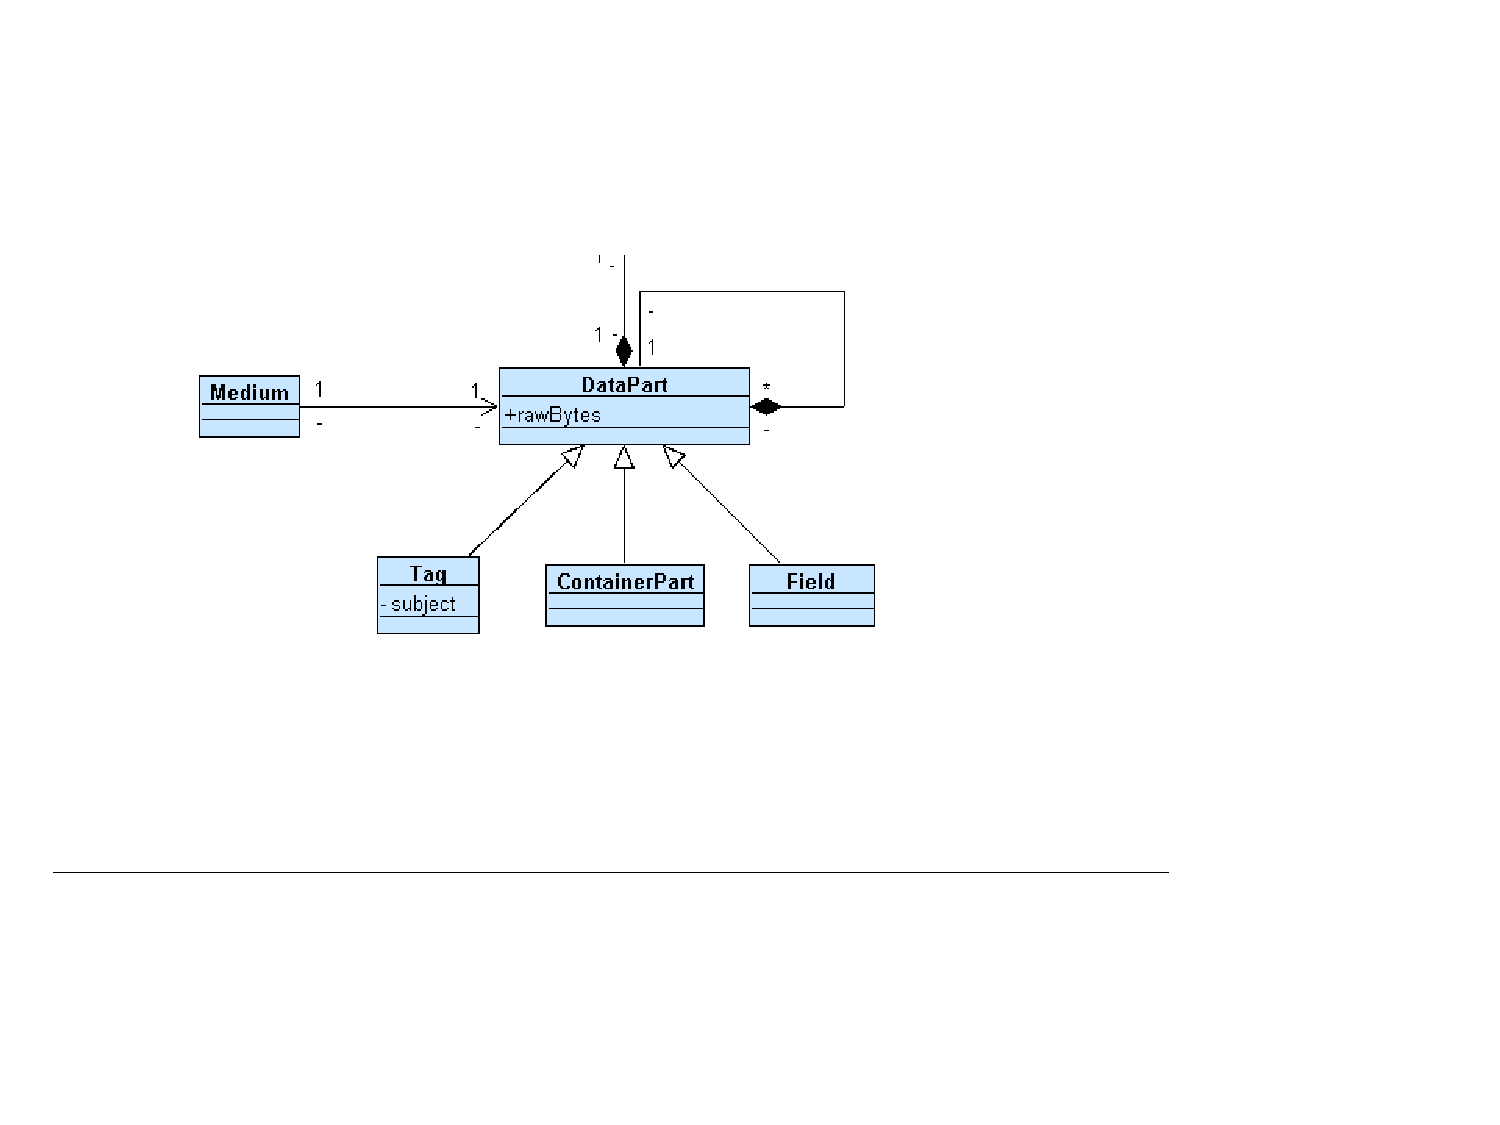
\includegraphics[width=1.00\linewidth]{figures/II_GeneralModel.pdf}
\caption{The container metamodel}
\label{fig:II_GeneralModel}
\end{figure}

%%%% DD --> %%%%
\DD{dd:500}
{% Title
Containers as basic top-level unit, containing nested containers
}
{% Short description
All data that can be processed by \LibName{} consists of containers. A container is a sequence of bytes with a specific structure belonging to exactly one container data format. However, consecutive containers might belong to different data formats.

In addition, a container - as the name suggests - contains other data. This data might be containers of the same format again. The nesting might be arbitrarily deep. A nested container is able to contain data of other formats. 
}
{% Rationale
Every format considered here has such basic building blocks, called differently in each format specification (atom, frame, page, element, item, tag etc.). The same file or media stream might consist of containers belonging to different formats. One example is an MP3 file with an ID3v2 tag. See also \cite{MC17}, part IV for more details.

Most of the supported data formats have some notion of nesting child containers (or, for metadata formats: attributes) within parent containers. Those child containers have either exactly the same stucture as the top-level containers, or they differ slightly. Some formats such as RIFF explicitly define specific containers that embed data belonging to other metadata formats. 
}
{% Disadvantages
No disadvantages known
}
%%%% <-- DD %%%%

How are these containers structured in detail?

%%%% DD --> %%%%
\DD{dd:501}
{% Title
A container consists of an optional \textbf{header}, \textbf{payload} and an optional \textbf{footer}
}
{% Short description
Every container - no matter which data format - follows the same basic structure: One or more optional headers start the container's byte sequence. Following this, there is a sequence of bytes called the payload. At the end of the container, there are one or more optional footers. A container must either have at least a single header or at least a single footer.
}
{% Rationale
Considering table \ref{tab:DFcompareMult} and \ref{tab:DFcompareMeta}, every container in every format has at least one header or one footer, including nested containers. Only ID3v23 as sole exception has a second, so-called extended header. Thus we have to support multiple headers and footers, even though this might be a singular case. But future formats might come to bring multiple headers, too. Modelling the middle part of a container as payload explicitly instead of just as list of sub-containers or fields makes sense because it allows to lazily read substructures, or entirely skip the payload.
}
{% Disadvantages
No disadvantages known
}
%%%% <-- DD %%%%

We saw that containers have a structure, and containers can live within other containers. But on the lowest level, there are leaf nodes, the fields:

%%%% DD --> %%%%
\DD{dd:502}
{% Title
Fields as the atomic unit of all byte sequences
}
{% Short description
\textbf{Field}s are the leaf nodes of the container metamodel: A field is a sequence of 1 to N consecutive bytes. A field has a \textbf{binary value} as well as an \textbf{interpreted value}, i.e. a human-understandable value with a specific meaning. We say that a field has a specific type, which basically describes the mapping between binary and interpreted value as well as the allowed values or format of a field.
}
{% Rationale
The term ``field'' is quite commonly used in binary data formats. It does not make sense to go down to individual byte or bit level. The smalles level of semantic in every binary or textual format is a field.
}
{% Disadvantages
No disadvantages known
}
%%%% <-- DD %%%%

Now towards headers and footers: Are they inherently different or basically the same? Fixed or variable size?

%%%% DD --> %%%%
\DD{dd:503}
{% Title
Headers and footers as sequences of fields are structurally identical
}
{% Short description
Headers and footers are sequences of fields, i.e. they must not nest a container. They are either variable or fixed-size. For both header and footer, the same model class called \texttt{Header} is used.
}
{% Rationale
No data format specifies a header or footer nesting a container-like data structure, they all consist of plain fields. Despite the location (before or behind the payload), there is nothing really distinguishing headers or footers from a structural perspective. Thus the same model class can be used for both. However, there is no english term for that class that seems to clearly be a grouping term for headers and footers.
}
{% Disadvantages
No disadvantages known
}
%%%% <-- DD %%%%

So far, we just introduced containers, fields, headers, footers and payload. We learned that containers might embed other containers, while headers and footers must only consist of fields. But what about the structure of the payload of a container? Of course, if the headers and footers cannot embed child containers, they must hide within the payload. Is this the only possibility? Of course not:
%%%% DD --> %%%%
\DD{dd:504}
{% Title
Payload either solely consists of containers or fields
}
{% Short description
The payload of a container either fully consists of a sequence of child containers or of a sequence of fields, but never both.
}
{% Rationale
Ultimately, we must boil payload down of fields, or put otherwise: We cannot recurse indefinitely into sub-containers. So at last, there must be a final sequence of child containers having payloads solely consisting of fields. So it is clear that we have both cases. But what about the mixed case: Should we have containers in the model that have both child fields neighbouring child containers? In rare cases such as - again - ID3v2, it would be possible to think of having the frames as child containers of the tag, followed by the padding child field of the tag behind it. However, we avoid such complexities, but payload is either ContainerBasedPayload or FieldBasedPayload. See next design decision of how we handle the ID3v2 special case.
}
{% Disadvantages
No disadvantages known
}
%%%% <-- DD %%%%

How to handle padding? If we look at the data format comparisons in \ref{tab:DFcompareMult} and \ref{tab:DFcompareMeta}, we see that padding is just a special case in ID3v2 and MP3. All other formats solve it ``more naturally'' by embedding it in special child container. ID3v2 just adds some nullbytes at the end of the tag payload behind the frames. How to model this? There are basically three possibilities:
\begin{itemize}
\item The padding is a part of the payload, basically a field. This seems most intuitive, but is already excluded by the previous design decision, because then we would need to support mixed payloads, consisting both of child containers and fields.
\item The padding is part of the payload, but considered as a very special child container.
\item The padding is an optional part of the tag footer.
\end{itemize}

Based on these alternatives, we can really only decide the following:
%%%% DD --> %%%%
\DD{dd:505}
{% Title
Padding in ID3v2 is modeled as very special child container of the tag
}
{% Short description
Padding in ID3v2 is modeled as very special child container of the tag, where the header is the first null byte, and all follow-up bytes form the payload. Note that for this to work, \LibName{} must support containers with no (i.e. empty) payload for the very special case that the padding only consists of one byte: The header magic key identifying the padding. 
}
{% Rationale
Modeling it as child field of the payload is not possible as it would contradict \DesLink{dd:504}. Modeling as part of the footer would be odd, as not every version of ID3v2 defines a footer at all, and we would have a variable sized footer optionally starting with an arbitrary number of nullbytes, which would not be very intuitive from a library users perspective, too.
}
{% Disadvantages
The only disadvantage possibly to be identified that there could be padding just consisting of a single byte. This would mean we'd have a container with just a header, but an empty payload, which actually is quite degenerate.
}
%%%% <-- DD %%%%

The overall term for containers, headers, footers, fields and payload is a \textbf{datablock}. This term is used further on throughout this document.

There is another ID3v2 specific that we directly want to exclude here:
%%%% DD --> %%%%
\DD{dd:505b}
{% Title
ID3v2 transformations such as unsynchronization, compression, encryption are not handled generically
}
{% Short description
ID3v2 is clearly overdesigned. It includes an outdated mechanism called \emph{unsynchronization} to ensure players do not interpret ID3v2 tags as MP3 frames and try to play them. ID3v2 also defines frame-based compression and encryption possibilities.

These facilities are not handled generically in \LibName{}, they are just specifically implemented in the ID3v2 extensions.
}
{% Rationale
Unsynchronization is not needed anymore, as current players all know about ID3v2 tags. Even if it would be needed: There is no other data format know to date that defines any such transformation schemes, not even for compression or encryption.

Thus, declaring this all as generic concept is useless as only one format defines such things, and these things are even only very rarely used.
}
{% Disadvantes
No disadvantages known
}
%%%% <-- DD %%%%

% =======================================================================================================
\subsection{Representing a Data Format}%
\label{sec:RepresentingaDataFormat}%

Data Formats need some kind of representation:
%%%% DD --> %%%%
\DD{dd:506}
{% Title
Class for data formats and especially for container formats
}
{% Short description
There is a base class called \texttt{AbstractDataFormat} representing a general data format, which has a subclass called \texttt{ContainerDataFormat} that is used for all data formats listed in \SectionLink{sec:FormatComparison}. Each individual format is represented as an instance of \texttt{ContainerDataFormat}. These two classes are neither enums nor ``dynamic enums'', but just plain old java classes.
}
{% Rationale
We need some way to identify which data format a container belongs to. A class allows to store additional format-wide properties for logging or even with a functional notion behind. Why not using an enum to identify each supported data format? Because enums are static, and we do not want to change the enum whenever a new format comes around. And it is not clear which formats are out there by 3rd party. A dynamic enum pattern is unnecessarily complexity here, so just a plain class. Why a just an instance of \texttt{ContainerDataFormat} rather than a new subclass for each format supported? First of all, data formats must be used as tokens by end-users of the library to refer to which tags or containers they want  to read. Creating a new sub-class instance everytime they want to have a token is strange. Instead, they can use a public constant instance as token. The next question: Why at all a \texttt{ContainerDataFormat} subclass? The reason is that \LibName{} might want to support even more different formats in future, e.g. XML. This can be a sibling subclass of \texttt{AbstractDataFormat}. From now on, everything described in this section is only covering container data formats.
}
{% Disadvantes
No disadvantages known
}
%%%% <-- DD %%%%

But that's not all of it. If we structure data belonging to a format into containers, headers, footers and so on according to the generic metamodel, \emph{how exactly} is a correct datablock of a given format structured? Of course, each format individually specifies the exact structure of its containers (how many headers, footers etc., what the payload can contain), headers (which fields make up a header), fields (which type a field has, how long it is and which values it can have) and so on. Thus, we need a place where we describe the structure of all datablocks belonging to a data format in more detail, otherwise we could not parse this data generically.

We define:
%%%% DD --> %%%%
\DD{dd:507}
{% Title
\texttt{DataFormatSpecification} provides \texttt{DataBlockDescription}s, \texttt{DataFormatRepository} maintains all \texttt{DataFormatSpecification}s
}
{% Short description
The exact properties of a datablock is described by an instance of the class \texttt{DataBlockDescription}. Which properties are needed in detail is determined later in \SectionLink{sec:DatablockProperties}.
The interface \texttt{DataFormatSpecification} provides access to all \texttt{DataBlockDescription}s offered by one specific data format. Last but not least there is a \texttt{DataFormatRepository} interface which basically only maintains a list of all supported data formats and their corresponding \texttt{DataFormatSpecification}s.

A concrete \texttt{DataFormatSpecification} is defined in an extension and loaded when starting \LibName{}. 
}
{% Rationale
For generically parsing data blocks according to a format definition, the parser code needs information about the exact structure of a data block. Thus, we need a place to maintain all data formats, their specifications and a description of each possible individual container, field etc.
}
{% Disadvantes
No disadvantages known
}
%%%% <-- DD %%%%

% =======================================================================================================
\subsection{\texttt{DataBlockDescription} Common Properties}%
\label{sec:DatablockProperties}%

First of all, we need a clear way to identify each specific datablock that might occur in the data format. Every container type, header, footer, field and payload needs an identifier:
%%%% DD --> %%%%
\DD{dd:508}
{% Title
Each datablock of a format has a specification id unique across all supported formats
}
{% Short description
Each distinctly defined container, header, footer, field or payload block of a data format is assigned a unique specification id. Using this specification id, a parser implementation can lookup the \texttt{DataBlockDescription} of the block from its associated \texttt{DataFormatSpecification}. Specification ids are human-readble rather than generated GUIDs. The uniqueness is guaranteed by using a top-level prefix identifier that is directly checked to be unique upon all loaded data formats when loading the extension defining the data format. The ids reflect the hierarchical nature of a data format according to the container meta model, following these rules:
\begin{itemize}
\item Each id consists of one or more \emph{segments} separated by a dot.
\item A segment name does only contain ASCII alphanumeric characters, starting always with a lower-case letter and preferring lower-case only letters, i.e. no special characters, no blanks etc. So a datablock id has much in common with a Java package name. 
\item The first segment is the data format top-level prefix which equals the (single) top-level container id of the data format. So we have the implicit decision that each format starts off with a single container on top-level enclosing everything else. This is true for all data formats considered here.
\item Each container consists of an arbitrary number of headers and footers as well as exactly one payload. The segment name of a container payload is always \texttt{payload}. If there is just a single header or footer, it is called header or footer respectively. Multiple headers or footers bear more specific, distinct names.
\item Child fields of a header or footer have descriptive names and so on 
\end{itemize}
}
{% Rationale
When parsing, the format structure of a datablock must be clearly visible and available. By an id, this format structure is clearly adressable and the corresponding \texttt{DataBlockDescription} can be obtained from a \texttt{DataFormatSpecification}. The uniquenss of the id guarantees that the parsing logic cannot unintentially try to parse a block of bytes according to the incorrect format.

The reason for not using generated unique ids such as counters or GUIDs is that we want to have memorable and recognizable names, both for library developers (e.g. during debugging) or \LibName{} end-users that need to work with datablock ids directly. 
}
{% Disadvantes
No disadvantages known
}
%%%% <-- DD %%%%

Besides their id, what else might be desirable on first glance when looking at a datablock taken from a data format's specification? Some descriptive stuff comes to mind. Second, it seems like every datablock must have exactly one type that is useful to store. So we can state:
%%%% DD --> %%%%
\DD{dd:509}
{% Title
Basic properties held in a \texttt{DataBlockDescription}
}
{% Short description
Each \texttt{DataBlockDescription} instance holds the datablock id of the datablock according to \DesLink{dd:508}. In addition, it has:
\begin{itemize}
\item A more human-readable name of the datablock, if available; only for display or documentation purposes
\item A description of the datablock, probably taken from the format specification, preferably in English. This is meant to give more information about the purpose of the datablock, but has no other meaning.
\item The \texttt{DataBlockType} of the datablock, which is: \texttt{HEADER}, \texttt{FOOTER}, \texttt{CONTAINER}, \texttt{FIELD}, as well as \-- according to \DesLink{dd:504} \-- \texttt{FIELD\_BASED\_PAYLOAD} or \texttt{CONTAINER\_BASED\_PAYLOAD}.
\end{itemize}
}
{% Rationale
These properties are clear from the beginning, the concrete is known statically, and it is needed to take decisions during generic parsing. 
}
{% Disadvantes
No disadvantages known
}
%%%% <-- DD %%%%
 
We defined that datablock ids are organized hierarchically as their real blocks are organized hierarchically. However, still, it is not sufficient to somehow maintain the ``hierarchy'' indicated by the metamodel only in the datablock ids. Instead, we define:
%%%% DD --> %%%%
\DD{dd:510}
{% Title
\texttt{DataBlockDescription}s contain a list of all child ids they might contain, where order matters
}
{% Short description
A \texttt{DataBlockDescription} instance contains a list of all child datablock ids that form the structure of the datablock described. While headers, footers, containers and payload usually has child ids, \texttt{DataBlockDescription}s of fields must not define child datablock ids. The list of child ids is ordered with the following meaning:
\begin{itemize}
\item For containers, the child id list exactly matches the correct order of headers, payload and footers that build the container
\item For headers, footers and field-based payload, the child id list exactly matches the order of child fields within the header, footer or field-based
\item For container-based payloads, the child id list order does not have a meaning, i.e. if multiple different container types are allowed, they might appear in any order 
\end{itemize}
}
{% Rationale
The parsing code somehow needs information about what child blocks of which format to expect within a given datablock, otherwise parsing it correctly is simply impossible. Each data format clearly defines the order of fields, headers and footers. Usually, most container formats define just exactly one child container that can appear in a container-based payload. However, there are cases such as QuickTime (atom vs. QT atom container) that define multiple different container types that might appear in any possible order. 
}
{% Disadvantes
No disadvantages known
}
%%%% <-- DD %%%%

We first have to define some limitations for these datablock ids that should be made clear:
%%%% DD --> %%%%
\DD{dd:511}
{% Title
Datablock ids and their segments MUST not be used for any logic 
}
{% Short description
Especially, no assumptions about the hierarchical relations of distinct blocks must be done based on their id. E.g. a block with specification id \texttt{id3v23.payload.talb.encoding} not necessarily is a child of a block with id \texttt{id3v23.payload.talb}, as there could be multiple \texttt{talb} containers within an ID3v23 tag. So datablock ids are only specification ids, not instance ids! Even within the same specification, a case might occur where the same chunk of data with the exact structure appears in several places, e.g. as child of the top-level container, and also as deeper nested child. Moreover, some container formats encourage to embed datablocks belonging to even completely different data formats. How do we handle such cases? In no special way. Even if a container might appear on several levels, we just define its structure once in the data format with just one id. And if a datablock of a data format is embedded in another container of a different format, it still keeps its well-defined datablock id according to its data format. So this again shows that based on the id, we can never determine the real hierarchy level or instance relations of two datablocks during parsing! 
}
{% Rationale
Quite clear, otherwise we would implement a lot of bullshit code
}
{% Disadvantes
No disadvantages known
}
%%%% <-- DD %%%%

% =======================================================================================================
\subsection{Generic and Concrete Containers}%
\label{sec:ConcreteandGenericContainers}%

Data formats define different kinds of \emph{container types}. A container type for us is defined as a data structure having a fixed number of headers and footers, where each header and footer has a strictly defined sequence of fields with strictly defined syntax and semantics, yet leaving undefined how the payload looks like. They just state that there is a payload consisting of bytes, but not how it is structured. Most often, there is just one header or just one footer. Here are some examples of container types:
\begin{itemize}
\item Most container formats such as RIFF or Matroska define exactly one container type. In these formats, those containers usually can be found on top-level as well as arbitrarily nested within parent containers   
\item Some formats that are no container formats in the narrower sense\footnote{In terms of their main purpose is to contain \emph{arbitrary} multimedia data, not only data of a specific kind.} such as ID3v23 use a slightly different container type for the top-level (the tag) container as for the child (the frame) containers 
\item Some container formats such as QuickTime even define multiple container types that can appear on the same level: First of all, there are the top-level containers called atoms; one extension of atoms are QT atoms, which just use a slightly extended header compared to the usual atoms. Both might appear on top-level. Furthermore, as child container types, not only atoms or QT atoms might appear, but also QT atom containers (a slightly confusing term here, but this is how QuickTime names them)
\end{itemize}

Container types are the pillars of the most basic property of most well-designed container formats: They define the structures of their basic buildings blocks (i.e. their container types) just once, and specialize this basic structure whenever needed. This at first allows to write generic parsers that may skip containers whose semantics and purpose they might not be aware of, but yet they still know their structure and thus are able to determine where the next container actually starts. This allows to extend data formats by new subtypes whereas existing parsers still work.

But this is not yet enough. Most container formats go much farther than only define a generic container type that can be parsed and defines a structure. They specialize in terms of defining specific containers having a specific meaning (data content) and whose payload follows a deeper defined format. These specialized containers can be said to have the same structure as a given container type, but they fill this container type with meaning and the payload with additional structure.

We define:
%%%% DD --> %%%%
\DD{dd:512}
{% Title
\COMPdataFormatManagement{} distinguishes generic and concrete containers
}
{% Short description
\COMPdataFormatManagement{} distinguishes generic and concrete containers:
\begin{itemize}
\item A container is called a \textbf{generic container} if it is just known to follow a container type's structure, but a more specialized container type is not (yet) known; more technically speaking: A generic container is a container whose detailed payload structure is not yet known in advance, but can only be determined at runtime, usually by reading some specific \texttt{id} field of the container's header or footer. Examples for generic containers are: Generic ID3v23 frame, generic (QT) atom, generic Matroska segment, generic APEv2 item and others. We can say that generic containers form the archetypes for the even more useful concrete containers. \COMPdataFormatManagement{} must maintain \texttt{DataBlockDescription}s for generic containers.
\item A \textbf{concrete container} is a container with a well-defined payload structure. It might be based on a generic container which means it entirely inherits its header and footer structure, while it might ``override'' specific field values in headers and footers. Examples for concrete containers are: ID3v23 tag (because its payload structure is already statically clearly defined), ID3v23 TALB frame, ID3v23 GEOB frame, moov QT atom, APEv2 title item and others. \COMPdataFormatManagement{} must maintain \texttt{DataBlockDescription}s for concrete containers. 
\end{itemize}

Of course, there are much more concrete containers than there are generic containers.
}
{% Rationale
Generic containers are necessary such that \LibName{} can basically parse data format content, yet not necessarily understanding its payload. These ``unknown'' containers can safely be skipped, and \LibName{} can later be extended to also understand these concrete types.

Concrete containers are necessary such that \LibName{} can read and write data with specific semantics and inner structure. Otherwise it would not be possible to write album, track, artist etc. fields to metadata container formats and so on.
}
{% Disadvantes
No disadvantages known
}
%%%% <-- DD %%%%

How exactly are these generic and concrete container \texttt{DataBlockDescription}s defined in a \texttt{DataFormatSpecification} and used at runtime?

%%%% DD --> %%%%
\DD{dd:513}
{% Title
\texttt{DataFormatSpecification}s list generic container as children, parsers resolve them to concrete containers at runtime
}
{% Short description
Generic container types might occur on arbitrary levels of the data block hierarchy, either on top-level or as child datablocks of a \texttt{CONTAINER\_BASED\_PAYLOAD} datablock. The semantics is: The file/media stream or payload contains a sequence of containers having a specific basic structure (i.e. they have a specific container type). This type can be found to be even more specific at runtime. For this, container formats define a special id field either in the container header or footer. This id field identifies the concrete type of container. After the parser has read the id field, it can lookup if there is a more specific \texttt{DataBlockDescription} for this id defined in its \texttt{DataFormatSpecification}. If so, the generic container is changed to the concrete container, thus the payload can now be parsed differently. 
}
{% Rationale
All container formats define their \texttt{CONTAINER\_BASED\_PAYLOAD} to contain a multitude of different concrete containers that all follow (usually) a single generic container type.
}
{% Disadvantes
No disadvantages known
}
%%%% <-- DD %%%%

The actual detailed parsing process is described within the design of \COMPdataPartManagement{}.

Now we already mentioned in \DesLink{dd:513} that there is ``usually'' only a single generic container defined within a \texttt{CONTAINER\_BASED\_PAYLOAD}. However, there are also already two exceptions we can list here:
\begin{itemize}
\item A (QT) atom generic container having a \texttt{CONTAINER\_BASED\_PAYLOAD} could have two different generic container types as child containers: Either (QT) atoms again, or QT atom containers that have a totally different header. 
\item We already ``artificially'' introduced a second case with \DesLink{dd:505}: An ID3v23 tag \texttt{CONTAINER\_BASED\_PAYLOAD} either contains a generic ID3v23 frame or a padding container.
\end{itemize}

If a \texttt{CONTAINER\_BASED\_PAYLOAD} might contain different types of containers in arbitrary order, how is a parser able to tell which generic container type he is handling currently? This is all based on magic keys and described in \SectionLink{sec:MagicKeys}.

% =======================================================================================================
\subsection{Data Format Identification and Magic Keys}%
\label{sec:MagicKeys}%

This section deals with the question how to identify that a given chunk of bytes belongs to a specific data format. This is not an easy thing because of the following aspects:
\begin{itemize}
\item There are different media types such as files, continuous streams and in-memory bytes
\item Different strategies of reading data formats are (partly) supported in \LibName{}: Most data formats are designed for the default way of reading, i.e. \textbf{forward reading} starting from the beginning of the medium from offset zero towards higher offsets. However, sometimes \textbf{backward reading} is much more performant, especially for multimedia tags. Last but not least, you can think of \textbf{scanning} to search a chunk of bytes for the first occurrence of a known format.
\item Some data formats are extremely similar to each other, either due to the fact that they are different revisions of the same family of formats (e.g. ID3v23 and ID3v24) or due to decisions of standardization boards (e.g. the ISO base multimedia format with its children JPEG 2000, MPEG-4 and others which are nearly identical to QuickTime) - how to distinguish them.
\item A few data formats such as MP3 allow coexistence of multiple unrelated data formats on top-level of a medium, usually a file. An MP3 file not only contains MP3 frames, but also ID3v1, ID3v3, LyricsV3 or APE tags, all of which are entirely different data formats specified on their own. This is a special case as most other multimedia data formats such as RIFF, QuickTime, Matroska and Ogg require to only have data blocks of RIFF, QuickTime, Matroska and Ogg on top-level in the same medium.
\end{itemize}

What are the different possibilities of identifying the data format of a medium?
\begin{itemize}
\item \emph{Based on the file extension:} In 80 percent of the cases, you could think of identifying a data format based on its file extension. This requires a mapping of extensions to data formats. While this could be a feasible approach, its downsides are clear: If the file has no extension (e.g. on Unix systems this could be the case), you cannot identify it. Furthermore, this approach is not feasible for streaming media and in-memory bytes.
\item \emph{Using other external hints:} You can use other external hints, e.g. external metadata (provided in separate files, in an HTTP header for streams) or let the user select or hint at the data format. Obviously, this could never be a possibility covering all cases and requires a lot of very diverse strategies to implement. 
\item \emph{Based on information in the data:} You read the bytes and try to identify the data format based on the bytes in the data itself. Mostly, this translates into using magic keys which we will cover immediately or scanning. While this might seem strenuous, it is actually the only proven way to ensure proper identification that even works for all different media.
\end{itemize}

So we decide:
%%%% DD --> %%%%
\DD{dd:520a}
{% Title
Default identification mechanism uses magic keys
}
{% Short description
\LibName{} uses magic keys to identify the data format of a given chunk of data bytes. Scanning is not used for identifaction for now.
}
{% Rationale
Its the only reliable way to identify a data format, and we anyway need to parse the data. It works for all media types. Regarding scanning:  It is currently excluded, see \SectionLink{sec:EXCL005Scanningfordataformatsnotsupported}.
}
{% Disadvantes
No disadvantages known
}
%%%% <-- DD %%%%

Now we want to deal with the very basic and central concept common to most if not all of those data formats: \textbf{Magic Keys}. A magic key is a sequence of bytes with a fixed, well-known value, which allows to identify a block of bytes as belonging to a data format, enabling generic parsers to understand how to parse a byte sequence. Thus, it is usually located at the start of the medium. For example, an Ogg page is identified by the magic key string ``OggS'', encoded as ASCII. Of course, this implies that different data formats use different magic keys.

These are the main properties of magic keys we are most interested in:
\begin{itemize}
\item A magic key has a single fixed byte identification sequence that is usually an ASCII encoded string
\item It is either starting at the beginning of a container, or at a well-defined fixed offset from the start of the container, thereby being a field in the container's header or footer
\item That said, also footers have magic keys to be used for backward reading, e.g. for ID3v23, APEv2 or Lyrics3v2
\item Data formats might have multiple magic keys identifying them - one example is RIFF where the magic key also identifies the byte order of the container
\end{itemize}

Let's list all magic keys of the data formats we care about in table \ref{tab:magicKeys}.

\begin{longtable}{|p{0.2\linewidth}|p{0.35\linewidth}|p{0.35\linewidth}|}
\hline
\rowcolor[gray]{.9}\textbf{Data Format} & \textbf{Header Keys} & \textbf{Footer Keys} \\
\endhead
\hline
Ogg  & ``OggS'' at start of page header & -  \\
\hline
Matroska  & 1A45DFA3h & -  \\
\hline
RIFF  & ``RIFF'' (big endian) or ``RIFX'' (little endian) at start of chunk header & -  \\
\hline
AIFF  & ``FORM'' at start of chunk header & -  \\
\hline
QuickTime  & ``ftyp'' or ``moov'' or ``pnot'' or ``mdat'' or ``skip'' as atom type (starting with 5th byte) in atom header & -  \\
\hline
MP3  & Eleven 1 bits at start of frame header & -  \\
\hline
ID3v1 and ID3v1.1  & ``TAG'' at start of tag header & -  \\
\hline
ID3v22  & ``ID3'' followed by version number 0200h at start of tag header & -  \\
\hline
ID3v23  & ``ID3'' followed by version number 0300h at start of tag header & -  \\
\hline
ID3v24  & ``ID3'' followed by version number 0400h at start of tag header & ``3DI'' followed by version number 0400h at start of tag footer \\
\hline
APEv1  & ``APETAGEX'' followed by version number 1000 at start of tag header & ``APETAGEX'' followed by version number 1000 at start of tag footer \\
\hline
APEv2  & ``APETAGEX'' followed by version number 2000 at start of tag header & ``APETAGEX'' followed by version number 2000 at start of tag footer \\
\hline
Lyrics3v1  & ``LYRICSBEGIN'' at start of tag header & ``LYRICSEND'' starting with 7th byte of tag footer  \\
\hline
Lyrics3v2  & ``LYRICSBEGIN'' at start of tag header & ``LYRICS200'' starting with 7th byte of tag footer  \\
\hline
VorbisComment  & \emph{No magic key} & -  \\
\hline
\caption{Magic keys of all relevant data formats}
\label{tab:magicKeys}
\end{longtable}

Let us look at the odd exceptions in this list:
\begin{enumerate}
\item [(1)] We see that the only format not having a magic key is the VorbisComment
\item [(2)] MP3 as the only format does not have a string magic key, but rather a bit sequence
\item [(3)] RIFF as the only format defines multiple different magic keys in its header
\item [(4)] Lyrics3v2 and ID3v24 are the only formats where header and footer magic keys differ
\item [(5)] QuickTime and Lyrics3v2 are the only formats where the magic key does not start at the beginning of its header/footer, but at a fixed byte offset
\item [(6)] QuickTime is very vague about its magic key, it actually defines all top-level atoms as optional, but recommends to usually start a QuickTime file with the ftyp atom
\item [(7)] Matroska seems to have an integer magic key
\end{enumerate}

Gradually, we will develop a strategy that includes all of those special cases.

First of all, we summarize and define:
%%%% DD --> %%%%
\DD{dd:520}
{% Title
A top-level container defines one or several magic keys in headers or footers 
}
{% Short description
Every top-level container must define one or multiple magic keys identifying the container and data format. The magic key is either at the start (header) or at the end (footer) of a container. We introduce a class \texttt{MagicKey} for describing the properties of a magic key. It defines:
\begin{itemize}
\item The magic key bytes
\item A bit length of the magic key
\item Optional: A string representation of the magic key
\item Optional: A fixed byte-length distance from start of header (positive) or end of footer (negative)
\end{itemize}
}
{% Rationale
Every top-level container must at least have one magic key, because otherwise we cannot identify it. The possibility of multiple different magic keys is implied by e.g. RIFF and QuickTime. ID3v24 defines a header magic key as well as a different footer magic key for backward reading. The bit length in contrast to a byte length is necessary for the MP3 magic key which is not a multiple of 8 bits, but 11 bits long. The fixed byte-length distance from start of header or footer is necessary for formats such as QuickTime. 
}
{% Disadvantes
No disadvantages known
}
%%%% <-- DD %%%%

Having defined this, we already covered the exceptions number (2), (3), (4) and (5). Now let's tackle QuickTime:
%%%% DD --> %%%%
\DD{dd:520b}
{% Title
ftyp, pnot, mdat and moov as magic keys for QuickTime
}
{% Short description
ftyp, pnot, mdat and moov are defined as the magic keys for QuickTime. If none of these atoms is found, a byte chunk cannot be identified as QuickTime.
}
{% Rationale
The vagueness of the specification is a problem, but we can reasonably handle it like that and be quite sure that in 90 percent of the cases, we can read QuickTime files properly.
}
{% Disadvantes
Some very special QuickTime byte sequence might not be readable with \LibName{}.
}
%%%% <-- DD %%%%

Now we are left with the VorbisComment special case. Unfortunately, you need external context knowledge to just know that the chunk of bytes is a Vorbis Comment. As described in \cite[MC17]{MC17}:
\begin{itemize}
\item In Vorbis bitstreams, it always is embedded in the second page of the stream
\item In FLAC, Speex and theora bitstreams, it is always starting with the second packet of the stream, it is actually not quite clear if this is the same thing as for Vobis, but note that Vorbis says page and the other say packet which is conceptually different in Ogg!
\end{itemize}

The VorbisComment, to say it cleary, seems quite oddly designed. We will not invent a generic solution for this, thus we define:
%%%% DD --> %%%%
\DD{dd:521}
{% Title
VorbisComment oddities are only handled in the Ogg and VorbisComment implementations
}
{% Short description
The generic parsing algorithm of \LibName{} does not provide any support for data formats that have no magic keys such as VorbisComment. Instead, such oddities need to be handled in the individual implementations. We assume that this can be done quite easily in the Ogg and VorbisComment parsing implementations.
}
{% Rationale
Handling such a singular special case in a generic way is quite hard and would greatly complicate the generic parser. Implementations should be able to handle it with their special knowledge, which does not need to leak into the generic parser.
}
{% Disadvantes
No disadvantages known
}
%%%% <-- DD %%%%

We have already covered top-level containers and data format identification. But what about nested containers? Do they also need to have magic keys? In most cases, we have generic nested containers whose exact structure is only revealed at runtime during parsing, e.g. ID3v2 frames, RIFF chunks, Matroska elements and so on. Having an id that is always different, they usually do not qualify to contain magic keys. If all data formats would define a generic nested container type, all would be fine. But again, we have candidates for problems:
\begin{itemize}
\item QuickTime defines two different types of nested containers that have a completely different structure: atoms and QT atom containers
\item ID3v2 has an odd use of padding by defining it as special null bytes behind the payload and before the footer (if any), thus he have defined to treat padding as special container, see \DesLink{dd:505} 
\end{itemize}

Here, we can use magic keys to the rescue:

%%%% DD --> %%%%
\DD{dd:521}
{% Title
Nested containers define magic keys if not generic
}
{% Short description
Usually, nested containers are generic. Non-generic nested containers are allowed to define one or multiple magic keys in their headers or footers. 
}
{% Rationale
QT atom containers have 10 zero-bytes at start which can be used as magic key. Likewise, padding always must start with a zero byte which is then the magic key.

Parsers reading payload bytes of a top-level container can first check for the presence of any magic key bytes of defined child containers. Only if these are not found, the single generic child container is assumed to be present. 
}
{% Disadvantes
No disadvantages known
}
%%%% <-- DD %%%%

Note that there are still two problems with the formats to solve when doing it like this:
\begin{itemize}
\item QuickTime (again) defines atoms and QT atoms as generic container types that can also be nested containers. QT atoms start with the same structure as atoms, but add some header fields.
\item When parsing child content like defined in \DesLink{dd:521}, there is a special case for Lyrics3v2: Unfortunately, the payload size of this tag is not known in andvance, but its end is only identified by the magic key in its footer. This special case is treated in \DesLink{dd:550} in another section. 
\end{itemize}

So let us check how to handle yet another QuickTime oddity:
%%%% DD --> %%%%
\DD{dd:522}
{% Title
QT atoms can be identified at runtime
}
{% Short description
QuickTime as only format relevant for us defines two different generic container types: Atoms and QT atoms. Thus, we define these two types of generic containers and use the generic container identification schemes to handle the situation. At runtime, if a specific id is found, the atom type is known to be an atom or QT atom, and further parsing is going on correspondly. See \DesLink{dd:513} for the runtime concrete container identification.
}
{% Rationale
Luckily, QT atoms just extend the header of atoms and otherwise are structure the same way. Thus this mechanism will resolve the problem.
}
{% Disadvantes
No disadvantages known
}
%%%% <-- DD %%%%

Based on these definitions, we can be more detailed about the parsing strategies:
%%%% DD --> %%%%
\DD{dd:523}
{% Title
Parsing top-level containers (forward reading)
}
{% Short description
For top-level containers, the data format identification is the first thing that happens. Each data format must define at least one top-level container which can either be generic or concrete. Each top-level container type must at least define one header magic key that indicates presence of the format. If the current bytes match the magic key, the data format is identified. Further on, if the top-level container is a generic container, the runtime identification of its concrete type is following as defined in \DesLink{dd:513}. Data formats that require deviating behaviour (e.g. VorbisComment) can override some aspects of this behaviour.
}
{% Rationale
This is directly following from all previous design decisions
}
{% Disadvantes
No disadvantages known
}
%%%% <-- DD %%%%

For nested containers, forward reading basically works like this:
%%%% DD --> %%%%
\DD{dd:524}
{% Title
Parsing nested containers (forward reading)
}
{% Short description
For nested containers, no data format identification is needed. The data format defines all possible containers that might occur in the container-based payload of the parent container. Each of these containers can either be generic or concrete. Any defined nested container might define a magic key. The parser first gets all child containers of the current payload who have a magic key defined and  tries to match the current bytes with these magic key bytes. If they match, the child container is found. Further on, if the nested container is a generic container, the runtime identification of its concrete type is following as defined in \DesLink{dd:513}. If none of the child containers with magic keys match, the parser gets the \emph{default nested container} which can be obtained from the \texttt{DataFormatSpecification}, if set. If this is the case, the parser assumes that the next container is the default nested container, otherwise it cannot identify the next container. If a container is found and this container is generic, the runtime identification of its concrete type is following as defined in \DesLink{dd:513}. This might e.g. reveal that an atom (default nested container for QuickTime) is actually a QT atom of a concrete type, see \DesLink{dd:522}.
}
{% Rationale
This is directly following from all previous design decisions. We have to define a default nested container just because of QuickTime as sole exception defining two very similar generic nested container types.
}
{% Disadvantes
No disadvantages known
}
%%%% <-- DD %%%%

Now the topic of backward-reading containers is still open. Again, there is a special case here: ID3v1 has no footer, but still is actually backward-readable. The reasons: It is defined to always be at the end of the file. Even if it is not, it could still be identified, as it has a fixed length. This means we would just need to look for the header magic key at a fixed offset from the end of the tag. However, there is a rather hidden special logic that additionally needs to be applied: If you identify the presence of a container by its footer magic key, you yet have to still read backward to obtain its payload. In case of ID3v1, you have arrived at the header already, such that you actually need to read forward to get its payload. 

To handle this, again, we have two alternatives: Either bring this special case into the generic layer, e.g. by adding a field to the magic key, which points to the offset for backward reading. Or we handle it only in the ID3v1 implementation. A third esoteric possibility would be to have a fake ``footer'' in ID3v1, such that we could just say: Whenever backward reading is necessary, just rely on footers only. But this would be very artificial and would lead to other problems. As was the case previously, we decide: 

%%%% DD --> %%%%
\DD{dd:525}
{% Title
Backward-reading for ID3v1 is implemented in the ID3v1 parser
}
{% Short description
The special case for ID3v1 is not considered in the generic parser code, but it is specifically overridden for this purpose in the ID3v1-specific parsing code.
}
{% Rationale
This decision is in line with the other design decisions. We want to keep the basic concepts and generic parser code and classes clear and clean of single-format special cases.
}
{% Disadvantes
No disadvantages known
}
%%%% <-- DD %%%%

Now, finally, let us define how backward reading is working overall. It is just a feature meant to be used for tags at the end of file. You cannot backward-read MP3 frames or Ogg pages, because they have no footer, such that you would need to ``scan backwards'' which we do not want to do. The second thought about backward-reading: It only affects the top-level, and not nested containers. To summarize:
%%%% DD --> %%%%
\DD{dd:526}
{% Title
Parsing top-level containers (backward reading)
}
{% Short description
A prerequisite for backward-reading top-level containers is that the data format has a footer with a magic key. The user has to exyplicitly request backward reading. The parser checks if it finds a footer magic key for all backward-readable data formats, i.e. data format identification happens here. It starts reading bytes to compare at the end offset of the footer plus the magic key offset (i.e. it reuses the offset defined in the \texttt{MagicKey} class, which is negative in this case). If the read bytes match the magic key, the data format is identified. Further on, if the top-level container is a generic container, the runtime identification of its concrete type is following as defined in \DesLink{dd:513}. Data formats that require deviating behaviour (e.g. ID3v1) can override some aspects of this behaviour. Backward reading stops as soon as no further backward-readable data format could be identified.

It is not necessary to backward-read nested child containers. 
}
{% Rationale
This is directly following from all previous design decisions. The reason why nested containers do not require backward-reading: Once you know were a backward-read top-level container starts, you can again forward-read its nested children.
}
{% Disadvantes
No disadvantages known
}
%%%% <-- DD %%%%

Now we have to clarify how the parsing code can best access the information about magic keys. We decide:
%%%% DD --> %%%%
\DD{dd:527}
{% Title
Obtain \texttt{MagicKey}s from \texttt{DataBlockDescription}s of containers
}
{% Short description
For the parser code, \texttt{MagicKey}s can be obtained from a \texttt{DataBlockDescription} of a container data block. It offers a method for obtaining the backward-readable (i.e. footer) magic keys as well as a method for obtaining the forward-readable (i.e. header) magic keys.
}
{% Rationale
A magic key essentially belongs to a container. The top-level container \texttt{DataBlockDescription}s and the nested container \texttt{DataBlockDescription}s must anyway be available a the places where we need to parse them. By providing different methods for forward and backward reading, the intentions become very clear. Overall, it is most convenient for the parser code this way.
}
{% Disadvantes
No disadvantages known
}
%%%% <-- DD %%%%

Strongly connected to this is the question how to represent magic keys in a data format while avoiding redundancies. We already defined a specific class called \texttt{MagicKey} and methods for obtaining the magic keys for this, which is a good choice as it bundles all the relevant information (and nothing more) for the parser code. But in the end, a magic key is nothing but a header or footer field with a fixed value. Thus we define:
%%%% DD --> %%%%
\DD{dd:528}
{% Title
\texttt{MagicKey} instances implicitly derived from field \texttt{DataBlockDescription}s 
}
{% Short description
The \texttt{MagicKey} instances that can be queried by the parsing code are not defined/added in parallel to the field properties anyway needed. In contrast to this, a \texttt{DataDataBlockDescription} of type \texttt{FIELD} additionally contains a flag saying if it is a magic key or not. If this flag is set to true, all other properties of the \texttt{MagicKey} can implicitly derived from the other field properties and a plausibility check can happen. If one of the following plausibility checks is failing, the \texttt{DataFormatSpecification} is considered invalid. 
\begin{itemize}
\item A field marked as magic key must either have a fixed value, or it must be an enumerated field (i.e. with multiple alternative values).
\item The header that contains the magic key field must be either be the first header or the headers before it must be fixed length headers. For footers: The footer that contains the magic key field must be either be last footer or the footers behind it must be fixed length footers. Otherwise the field does not qualify as magic key, because it might have a variable offset from the start or end of its container and the \texttt{DataFormatSpecification} cannot derive the necessary offset from start or end of container.
\item For the same reason, we define for headers: The fields in front of the magic key field (if any) must all be fixed length fields. And for footers: The fields behind the magic key field (if any) must all be fixed length fields.
\item There must be only at maximum one header magic key field and only at maximum one footer magic key field
\end{itemize}
}
{% Rationale
Redundancy is avoided, and it is more convenient to define a concrete \texttt{DataFormatSpecification}, as we do not need to repeat ourselves.
}
{% Disadvantes
A \texttt{DataFormatSpecification} implementation must be slightly more complex to derive and check the necessary properties of the \texttt{MagicKey} instances.
}
%%%% <-- DD %%%%

There is a special case with MP3 here: It has an odd number of bits. This makes defining the magic key as single field very hard. Instead, it needs to be defined as flag field and cannot be derived automatically:

%%%% DD --> %%%%
\DD{dd:528b}
{% Title
MP3 magic key is added manually to the specification
}
{% Short description
The MP3 magic key with 11 one bits is added manually to the MP3 \texttt{DataFormatSpecification}. Thus \texttt{DataBlockDescription} offers a method for adding a header or footer magic key manually. So auto-derival of magic keys is not used for MP3.
}
{% Rationale
The odd bit length does not allow to define the 11 bit field as field on its own, but it needs to use flags, and flags do not have individual default values. Thus it is not possible in the generic code to derive the magic key for MP3 automatically. Instead, the field is not tagged as magic key, but it is manually created in the MP3 extension and added using the \texttt{DataBlockDescription} method.
}
{% Disadvantes
No disadvantages known
}
%%%% <-- DD %%%%

Last but not least, we want to discuss the topic of different data format versions and their magic keys. Specifically, one could ask: Does the version number belong to the magic key of a data format or not? We define:
%%%% DD --> %%%%
\DD{dd:529}
{% Title
Magic keys do not include a version number
}
{% Short description
Magic keys never include the version number of the data format, even if it directly follows or preceedes the magic key and it might appear as solution to the problem of how to distignuish similar data formats.
}
{% Rationale
First of all, a version number might be numeric, while magic keys are usually strings. Does the string representation of the version number would be slightly odd. Second and more importantly, it is actually a different field, and it could well be that a data format does not define the version field to be directly adjacent to the magic key field.
}
{% Disadvantes
No disadvantages known
}
%%%% <-- DD %%%%

% =======================================================================================================
\subsection{Inheriting and Overriding Datablock Structures}%
\label{sec:InheritingandOverridingDatablockStructures}%

TODO


% =======================================================================================================
\subsection{Occurrences and Sizes}%
\label{sec:Sizes}%

In this section, we discuss the topics of how often does a data block occur, and how long is it?

The ``how often'' (occurrences) part is treated as follows:
%%%% DD --> %%%%
\DD{dd:529a}
{% Title
\texttt{DataBlockDescription} contains minimum and maximum occurrences
}
{% Short description
For every data block, its \texttt{DataBlockDescription} can specify the number of occurrences by giving its minimum and maximum occurrences. The rules:
\begin{itemize}
\item Both must be set to a positive number, where only for the minimum occurrences zero is allowed
\item If both are set, minimum occurrences must be smaller or equal compared to maximum occurrences
\end{itemize}
}
{% Rationale
A few formats have fields that occur not only once, but multiple times sequentially. Some fields exist whose occurrence count instead of their length is given: Vorbis comment (number of user comments), APEv2 (number of items, in addition to size), Ogg (number of segments, which is equal to size, as each segment has one byte as length).
}
{% Disadvantes
No disadvantages known
}
%%%% <-- DD %%%%
 
For the size of a data block, we have basically three possibilities:
\begin{itemize}
\item The data block has a constant, fixed size which is always the same. Most fields have this property, but also static format containers such as ID3v1. 
\item The data block is a variable-size field and it is terminated, see \SectionLink{sec:FieldProperties} for more details about this case. This leads to variable-size headers, footers, payload and containers that have a variable size because one of their fields is a variable-size field.
\item The data block size is dynamically determined by a previously read field value or a combination of such field values. This case is further detailed in section \SectionLink{sec:FieldFunctions}.
\end{itemize}

For each case, we need the following:
%%%% DD --> %%%%
\DD{dd:529b}
{% Title
\texttt{DataBlockDescription} contains minimum and maximum byte length
}
{% Short description
\texttt{DataBlockDescription} allows to set a minimum and maximum length of the data block in bytes. Either the minimum length is set to a positive number (bigger than zero!) and the maximum length is set to ``unknown length'', or both are set to a positive number (bigger than zero), where the maximum length must be equal to or bigger than the minimum length.

The fixed size case is covered by setting both to the same value. Differing values have no specific influence for the parser, but can be later used for format validation of a chunk of bytes. If not set or the values differ, this is a signal that the data block is either terminated or its size needs to be determined dynamically using other field values.
}
{% Rationale
\LibName{} needs to be able to reflect both static sizes as well as dynamic sizes, and to be future-proof, it is also good to have differeng min and max sizes given for data format validation.
}
{% Disadvantes
No disadvantages known
}
%%%% <-- DD %%%%

How to deal with uncertainty? It is not always the case that lengths or counts are known. We want a constant here that clearly communicates
%%%% DD --> %%%%
\DD{dd:529c}
{% Title
Constant for undefined or unknown length and offsets
}
{% Short description
We define a constant in \texttt{DataBlockDescription} which has the meaning of an undefined or (yet) unknown length or offset. The value of this constant is the smallest negative long.
}
{% Rationale
This is e.g. necessary for fields with dynamic length or for relative offsets that cannot be computed due to dynamic lenghts. Having only one constant for all reduces confusion and still clearly communicates intent. Using \texttt{null} for undefined is not clearly communicating intent and is less readable. The reason for choosing the smallest negative long is: While offsets might get negative in some cases, lengths and counts never do. It is reasonable to assume that the negative relative offets we need in \COMPdataFormatManagement{} never reach the smallest long.
}
{% Disadvantes
No disadvantages known
}
%%%% <-- DD %%%%


We just cover one additional special case here: In \DesLink{dd:521} and the follow-up discussion, we already noted that Lyrics3v2 is somewhat special in terms of how to determine its payload size: It cannot be done before parsing it. Instead, it is only known to end when the footer's magic key is found. Thus it is kind of ``terminated''. In a first design, this was handled by some kind of special magic keys, so-called ``exclusion keys'' that where defined to state ``if you find this key, a container of the current type IS NOT present''. However, we decided to redesign this to be less odd:

%%%% DD --> %%%%
\DD{dd:529d}
{% Title
Lyrics3v2 payload size is determined by reading all children
}
{% Short description
Lyrics3v2 special case (no size indicator in header) is treated by reading all children until its footer. This is done for any data format where no payload size could be determined after reading the headers.
}
{% Rationale
This case is currently only known for Lyrics3v2, but the generic handling is not too complicated but rather simple, thus not requiring a custom implementation for Lyrics3v2 only.
}
{% Disadvantes
No disadvantages known
}
%%%% <-- DD %%%%

% =======================================================================================================
\subsection{Field Properties}%
\label{sec:FieldProperties}%

Now we look into properties that are specific to data blocks of type \texttt{FIELD}. Here, we cover other properties specific to fields. However, we do not cover the details of how field conversion (interpreted value to binary value and vice versa) is working and how some special cases of field interpretation are handled. This is a topic for the \COMPdataPartManagement{} component. 

We already covered sizes of data blocks (including fields) and we already defined one property of a field: It might be a magic key field, see \DesLink{dd:528}. The fields are the leafs of the data block hierarchy, thus, ultimately, they represent concrete values. While we could decide to treat them only as raw bytes, this is counter-productive as it would make parsing less convenient. Thus we define:
%%%% DD --> %%%%
\DD{dd:530}
{% Title
Fields have one of the types binary, string, numeric, string list or flags
}
{% Short description
Every field has a field type, and thus not only a \textbf{binary value}, but also an \textbf{interpreted value}. The field types are:
\begin{itemize}
\item \textbf{String:} The field's value is representing a string in a specific encoding.
\item \textbf{Binary:} The field's value is not further interpreted, i.e. the interpreted value is identical to the binary value of the field. I.e. this could be used to represent raw encoded bytes of a codec.
\item \textbf{String List:} The field's value corresponds to a list of strings.
\item \textbf{Numeric:} The field's value is representing a numeric value with a specific byte order.
\item \textbf{Flags:} The field's value is representing flags, i.e. a set of bit toggles, e.g. vital for parsing. 
\end{itemize}
}
{% Rationale
Parsers can directly read the interpreted values of the fields they need for parsing (e.g. sizes, flags or others) without needing to implement conversion to an interpreted value themselves. Interpretation should be kept inside the format specific code - in this case in the data format specification.

All of the field types of our reference data formats can be covered by these types.

The string list type is unfortunately necessary just for the sake of ID3v2.4. 
}
{% Disadvantes
No disadvantages known
}
%%%% <-- DD %%%%

First, we will care about the string and string list fields:
%%%% DD --> %%%%
\DD{dd:531}
{% Title
String fields and string list fields support termination characters and fixed character encoding as specific properties
}
{% Short description
A non-fixed-size string field or string list field can be terminated by a single termination character given in the field's character encoding known at parsing time. Second, a string field might have a fixed character encoding to be used. Both are optional properties.  
}
{% Rationale
String fields can be terminated by termination characters, this is needed e.g. in ID3v1 and ID3v23 data formats, where the actual number of termination bytes depends on the current character encoding. Thus, it is best to define a termination character and then decide at parsing time, which bytes according to the current character encoding are expected as termination bytes. For string lists, the termination character also acts as separator between different list entries. See also \DesLink{dd:532}.

Some specifications define fixed character encodings for specific string fields that might deviate from the data format's default character encoding.
}
{% Disadvantes
No disadvantages known
}
%%%% <-- DD %%%%

What about binary fields? Basically, they do not need any additional properties, but we want to make one thing clear about termination:
%%%% DD --> %%%%
\DD{dd:532}
{% Title
Binary fields do not support termination bytes
}
{% Short description
While string fields can define a fixed termination character, binary fields do not support termination bytes. 
}
{% Rationale
The reason is simple: Within our reference formats, there is no single case where a terminated field exists that is not a string field. 
}
{% Disadvantes
No disadvantages known
}
%%%% <-- DD %%%%

Numeric fields require a byte order such that their numeric value can be interpreted:
%%%% DD --> %%%%
\DD{dd:533}
{% Title
Numeric fields support a fixed byte order
}
{% Short description
Numeric fields define a fixed byte order to use during conversion. It is an optional property.
}
{% Rationale
To be convertible into a numeric value, the parsers need to have information about a byte order to use.
}
{% Disadvantes
No disadvantages known
}
%%%% <-- DD %%%%

For flags, it would be convenient to describe them in particular, e.g. which flags are there, where are they and what is their meaning. Thus we introduce a new class:
%%%% DD --> %%%%
\DD{dd:534}
{% Title
Flag fields require an instance of \texttt{FlagSpecification} that describes all flags in a flags field
}
{% Short description
The class \texttt{FlagSpecification} describes a flags field having following properties:
\begin{itemize}
\item The fixed byte length of the flags field
\item The positions (byte and bit adress) and unique names of flags together with their specification descriptions 
\item A byte order
\end{itemize}

It also supports multi-bit-flags.
}
{% Rationale
It is more convenient to access the flags, in contrast to doing bitwise OR and AND yourself.
}
{% Disadvantes
No disadvantages known
}
%%%% <-- DD %%%%

One question that could arise now is: Why do we not have ``enumerated fields''? Actually, we had them in a previous version. They could allow for an \emph{arbitrary} interpreted type, allowing the end user to map arbitrary objects to their byte representation for a field. Although this might seem very flexible and extensible, we explicitly decided to remove it:
%%%% DD --> %%%%
\DD{dd:535}
{% Title
No ``enumerated'' field type, but an enumeration property
}
{% Short description
There is no such field type called ``enumerated'', but only the already mentioned field types. Instead, every field has an additional property, basically a mapping that enumerates all possible interpreted values mapped to their unique binary interpretation. This way, it is still possible to provide a fixed value set for e.g. validation or specific conversions.
}
{% Rationale
The main problem with an explicit enumerated field type is its \emph{arbitrary} interpreted type. The runtime cannot know which type it is and requires very adventurous casting to get it done, or you need to write special code essentially duplicating the same logic for enums vs. concrete types. As we can still enumerate, this is fine. The only place where it hurts a bit are fields that are representing a Charset or a ByteOrder. Here it would be nice to have an enumerated field type as Charset or ByteOrder. However, it is simply possible to map bytes to string representations of Charsets and ByteOrders, i.e. having a String field instead.
}
{% Disadvantes
Maybe less flexibility for future demands and less support for actual object orientation
}
%%%% <-- DD %%%%

As we have these default field types, we can also define default field conversion mechanisms:
%%%% DD --> %%%%
\DD{dd:536}
{% Title
Default field converters for every field type
}
{% Short description
\COMPdataFormatManagement{} provides default field converters used to convert the binary value of a field into an interpreted value. It first looks if there are enumerated values and maps values accordingly. If there is no matching enumerated value, the converter provides a default appropriate conversion based on provided character encoding and byte order. There are two conversion methods:
\begin{itemize}
\item \texttt{toInterpreted:} Converts a binary value to an interpreted value, taking current character encoding and byte order as parameters
\item \texttt{toBinary:} Converts an interpreted value to a binary value, taking current character encoding and byte order as parameters
\end{itemize}

So we can implement the following default conversion mechanisms:
\begin{itemize}
\item String: Convert the string into bytes and vice versa according to the provided character encoding
\item Binary: Identical conversion
\item Numeric: Convert the number into bytes according to the provided byte order, assuming unsigned integer
\item Flags: Put the binary value into a Flags instance and vice versa
\end{itemize}
}
{% Rationale
Conversion is quite standardized according to the standardizes field types, this might cover at least 80 percent of the conversion cases. Conversions are relatively simple such that it is fine to keep them in \COMPdataFormatManagement{}.
}
{% Disadvantes
No disadvantages known
}
%%%% <-- DD %%%%

But standard converters are not enough. What happens if you need signed integers instead of unsigned? This is where a custom converter comes in:
%%%% DD --> %%%%
\DD{dd:537}
{% Title
\COMPdataFormatManagement{} allows to add custom converters for each field
}
{% Short description
Users may add custom converters to a field upon \texttt{DataFormatSpecification} creation. A custom converter is a property of the field.
}
{% Rationale
E.g. necessary for ID3v23 (sync-safe integers), Lyrics3v2 (numbers represented as characters) and Matroska (VINTs).
}
{% Disadvantes
No disadvantages known
}
%%%% <-- DD %%%%

Finally, some fields - no matter what type - have always the same static value. We join this requirement with the notion of a default value, i.e. a value to be preferred when it is not known which would be the right value of a field.
%%%% DD --> %%%%
\DD{dd:538}
{% Title
Each field has an optional default (interpreted) value
}
{% Short description
Each field has an optional default (interpreted) value.
}
{% Rationale
The default values are needed for fields with fixed values, and might be used to fill field values in cases where they are unknown.
}
{% Disadvantes
No disadvantages known
}
%%%% <-- DD %%%%


% =======================================================================================================
\subsection{Field Functions}%
\label{sec:FieldFunctions}%

Some fields contain values that are contributing to so-called \emph{parsing metadata}, i.e. metadata that is required to correctly read the contents of a container. Most prominent case is a size field which e.g. contains the size of the payload in bytes. When parsing the container, it is vital to know where the container ends and the next one starts. So this context information is necessary for reading. But how to implement generic reading if different data formats have different size fields? A second question that comes up is: How to ensure the size field is consistently updated if the payload size increases? Of course we could burden this to the user of the library. But there is an idea that solves both problems at once: \emph{Field functions}.

%%%% DD --> %%%%
\DD{dd:540}
{% Title
\LibName{} uses field functions to link parsing metadata fields with the target data blocks they refer to
}
{% Short description
 To ensure consistency of container content and parsing metadata, so-called field functions are used in \LibName{}. They represent a reference of a single field to one or multiple target data blocks of any type, supporting the following categories:
  \begin{itemize}
  \item \texttt{SizeOf}: The field contains the size of a single other data block
  \item \texttt{SummedSizeOf}: The field contains the summed size of several other data blocks that must be consecutive
  \item \texttt{PresenceOf}: The field indicates that an optional data block is present or not
  \item \texttt{CountOf}: The field contains the number of occurrences of a data block that might have multiple occurrences
  \item \texttt{ByteOrderOf}: The field contains the byte order of a data block
  \item \texttt{CharacterEncodingOf}: The field contains the character encoding of a data block
  \end{itemize}
}
{% Rationale
Formalizing connections between data blocks is at first allowing to ensure consistency and facilitates a generic parsing approach. The categories represent the most common types of parsing metadata encountered.
}
{% Disadvantes
Added complexity
}
%%%% <-- DD %%%%

Future functions might be introduced such as ``CRC of'', but this is yet to be planned.

How this generic parsing approach exactly works is described in \SectionLink{sec:ContainerContextInformation}.

Here we focus on the specification aspects of field functions. First of all, let's examine some sane validity criteria for each field function. Table \ref{tab:ffvalidity} is listing them.

\begin{longtable}{p{0.5\textwidth}|p{0.5\textwidth}} \hline
  \textbf{Field function} & \textbf{Validity criteria} \\ \endhead \hline
  \texttt{SizeOf} & Must be a numeric field; must refer to exactly one target data block \\
  \texttt{SummedSizeOf} & Must be a numeric field; must refer to at least two sibling data blocks which have the same parent; at most one of the target data blocks must have undetermined size (i.e. neither fixed size, nor terminated nor \texttt{SizeOf} function for it) \\
  \texttt{CountOf} & Must be a numeric field; must refer to a data block of type header, footer, container or field (i.e. not to payload) \\
  \texttt{PresenceOf} & Must be a flags field; must refer to an optional data block of type header, footer or field (i.e. not to payload or container) \\
  \texttt{ByteOrderOf} & Must be a string field \\
  \texttt{CharacterEncodingOf} & Must be a string field \\
  \caption{Validity criteria for field functions}
  \label{tab:ffvalidity}
\end{longtable}

%%%% DD --> %%%%
\DD{dd:541}
{% Title
\LibName{} enforces the validity criteria listed in table \ref{tab:ffvalidity} for field functions
}
{% Short description
The field functions supported by \LibName{} adhere to the validity criteria listed in table \ref{tab:ffvalidity}. That means that these criteria are checked at specification creation time and lead to runtime exceptions if not met.
}
{% Rationale
  These criteria ensure that an extension cannot use nonsense functional links which lead to arkward errors during parsing. Specifically for \texttt{SummedSizeOf}, forcing just at max one with undermined size is ensuring that there are now infinite loops during parsing.

  Why only these and not more? E.g. we could enforce that \texttt{SizeOf} refers only to dynamic size targets. This is not done because there could be formats defining a size as static in current version, yet still having a \texttt{SizeOf} field to refer to. Similar things could be said for \texttt{CountOf} and dynamic occurrences. One could force \texttt{ByteOrderOf} to refer only to numeric fields or \texttt{CharacterEncodingOf} only to string fields. However, this is not helpful as a specification might state the byte order or character encoding just once referring to all fields. 
}
{% Disadvantes
No disadvantages known
}
%%%% <-- DD %%%%

Now we are just left to discuss the complexities of the \texttt{SizeOf} field function and why we need a separate \texttt{SummedSizeOf} field function. The problem with the \texttt{SizeOf} field function is that in a lot of formats, the size is not only referring to exactly the payload or just another field, but in a myriad of cases to multiple objects which we call data blocks - here are those dreadful examples from our reference formats:
\begin{itemize}
\item The ID3v2.3 and ID3v2.4 tag size refers to the tag payload size (including padding) \emph{plus} the size of the extended header, if any 
\item The ID3v2.3 extended header size is the size of up to 3 fields that follow up the size field itself within the extended header
\item The ID3v2.4 extended header size is the size of the entire extended header including the size field itself
\item For RIFF and AIFF, a chunk's size field refers to the size of the form type field (fixed size of 4 bytes) \emph{plus} the size of the actual chunk's payload
\item In QuickTime file format, the atom size is the size of the whole atom considered as container, i.e. header \emph{plus} payload
\item In APEv2, the size field in header or footer is the size of the payload \emph{plus} the footer's or header's size, if present
\item In APEv1 and APEv2, the item size is the size only of the value, i.e. not including key or flags
\item For Lyrics3v2, the tag size includes the payload size \emph{plus} the size of the header 
\end{itemize}

If each and every format would use the very same strategy to determine the size of its payload, it would be nice. Instead, we see that nearly every format has its special case. Not to mention that MP3 and Ogg do not have size fields at all but rely on a more complex way of calculating the payload size based on combining multiple fields in the container header.

How to handle this overwhelming variety? First of all, from a specification point of view, we have to state:
%%%% DD --> %%%%
\DD{dd:542}
{% Title
\texttt{SummedSizeOf} field function in addition to \texttt{SizeOf} to support multiple consecutive target blocks
}
{% Short description
A \texttt{SummedSizeOf} field function refers to at least two data blocks that - however - must be strictly consecutive according to their specification. This has the meaning: This field is the \emph{summed size of all} the referenced data blocks, if present.
}
{% Rationale
This is cleary required from a data format perspective as outlined above. The question is why not to use \texttt{SizeOf} both for single and multiple fields? The special case turns out to simplify implementation.
}
{% Disadvantes
Of course, field function handling will get more complex due to this special case.
}
%%%% <-- DD %%%%

Other implications of this complexity are dealt with when designing the actual parsing process.

% =======================================================================================================
\subsection{Header and Footer Properties}%
\label{sec:HeaderProperties}%


% =======================================================================================================
\subsection{Container Properties}%
\label{sec:ContainerProperties}%


% =======================================================================================================
\subsection{Payload Properties}%
\label{sec:PayloadProperties}%

% =======================================================================================================
\subsection{Builder API}%
\label{sec:BuilderAPI}%

From all that has been said previously, it might already be clear that a \texttt{DataFormatSpecification} is a complex thing: We have data blocks of very different types, each type with its individual properties and corresponding validity aspects, organized hierarchically. If we want user to create this, this can get very nasty. Actually, in a first version, there was just a plain old java interface for creating a \texttt{DataFormatSpecification}: A lot of boiler-plate code, creating and populating collections, wiring parents and children, filling attributes that have no meaning for a type with their default values, filling up values such as lenghts for parents and children redundantly etc.

So this is not only a pain to write, but also a pain to read and maintain. Thus we introduced a builder API as a quantum leap in contrast to the original API:
%%%% DD --> %%%%
\DD{dd:550}
{% Title
Builder API for creating valid \texttt{DataFormatSpecification}s and \texttt{DataBlockDescription}s
}
{% Short description
\COMPdataFormatManagement{} provides a comfortable builder API for building a \texttt{DataFormatSpecification} from its individual \texttt{DataBlockDescription}s. It uses method names for providing data block type and if it is generic or not, method parameters for adding the local id, name and description, and nested methods for setting other properties and adding children to a data block. It removes a lot of boiler-plate code, ensures the user only sees the properties that are really valid for the given type, and wires parents and children as well as their ids correctly.
}
{% Rationale
The user can add a new \texttt{DataFormatSpecification} much more conveniently. Furthermore, the code remains short and readable (thus maintainable), still communicating only what happens without any noise.

In addition, we noticed the following interesting benefits of the builder API:
\begin{itemize}
\item The user is not required to directly depend on the implementation of \texttt{DataFormatSpecification}
\item Cloning of data blocks can be implemented and provided in an easier way
\end{itemize}
}
{% Disadvantes
The builder API of course needs to be built and maintained, it is a complex structure of interdepentend classes and interfaces with a lot of generics magic. 
}
%%%% <-- DD %%%%


%###############################################################################################
%###############################################################################################
%
%		File end
%
%###############################################################################################
%###############################################################################################
%-----------------------------------------------------------------------------------------------
%		\COMPdataPartManagement{} Design
%-----------------------------------------------------------------------------------------------

\section{\COMPdataPartManagement{} Design}
\label{sec:COMPdataBlockManagementDesign}

In this section, the design of the component \COMPdataPartManagement{} is described. Basic task of the component is to implement the actual generic parsing of data of a supported data format in a well-performing, yet flexible and extensible way.
% =======================================================================================================
\subsection{Basic Concept for Reading}%
\label{sec:BasicConceptforReading}%

In section \SectionLink{sec:RepresentingaDataFormat}, we discussed the approach that a data format is described in terms of a \emph{data format specification}, which basically is a description of how data is represented as a chunk of bytes in the data format. It breaks up such a chunk into different types of so-called data blocks that form a well-defined hierarchy (see \SectionLink{sec:TheContainerMetamodel}). Given such a specification and data block hierarchy, we define the following design decisions:

%%%% DD --> %%%%
\DD{dd:601}
{% Title
Data block instance classes defined in \COMPdataPartManagement{}
}
{% Short description
The instances for the different data block types are represented as Java classes in the \COMPdataPartManagement{} component which use the same names as in figure \ref{fig:II_GeneralModel}.
}
{% Rationale
As chunks of bytes are structured according to the metamodel and the data format specification describes them as such, it is quite clear the have to be instance of corresponding classes during parsing. These instances are also returned to the user and provide a clear, better-to-understand view on the data. Btw., having a metamodel but not transforming it into a class model seems to be quite nonsense.
}
{% Disadvantages
No disadvantages known.
}
%%%% <-- DD %%%%

%%%% DD --> %%%%
\DD{dd:602}
{% Title
Specification-driven Read Approach
}
{% Short description
Reading is heavily based on the description of the data format in its data format specification. The descriptions of lengths and types are used as basic assumption for parsing, especially magic keys for first identification.
}
{% Rationale
It is quite clear that otherwise, the data format specification would be quite useless and we would implement some data-format-specific and thus non-generic code again.
}
{% Disadvantages
Is it flexible enough? If we stick to a stiff specification, how to ensure that it is flexible enough for different data formats?
}
%%%% <-- DD %%%%

%%%% DD --> %%%%
\DD{dd:603}
{% Title
Reading and writing with \COMPmedia{}
}
{% Short description
Reading and writing is done using \COMPmedia{}, including use of its caching features.
}
{% Rationale
Again this is very clear.
}
{% Disadvantages
No disadvantages known.
}
%%%% <-- DD %%%%

Given these basic design decisions, we are ready to sketch a rough draft of how reading basically works. We first summarize the very fundamentals that we know this far:
\begin{itemize}
\item Data is represented as linear chunks of bytes whose structure is defined by the data format specification
\item The top-level data blocks for reading are containers
\item It is not clear which data format we have in front of us
\item A data block might get large, as we use long as data type (see \DesLink{dd:417})
\end{itemize}

Given the first two observations, we define the following:

%%%% DD --> %%%%
\DD{dd:604}
{% Title
Iterator approach for reading
}
{% Short description
  \LibName{} provides an iterator pattern for iterating top-level containers.
}
{% Rationale
As the basic structure of a chunk of data format bytes consists of linear disjoint containers and we need to do forward-reading, an iterator is a quite natural choice. Lists or other collection data types would be insufficient, because they would suggest that there is a finite number of containers. Iterators are a good fit for streaming, allowing virtually ``unlimited'' streams of containers.
}
{% Disadvantages
No disadvantages known.
}
%%%% <-- DD %%%%

Now we can define the basis approach of forward reading, i.e. what is done if we read a top-level container? Of course, first it is not clear which data format we have - identification is necessary, already introduced in \SectionLink{sec:MagicKeys}. Second, it might happen anytime that we hit end of medium, either expectedly or unexpectedly. The basic flow is defined in the following design decision and shown in figure \ref{fig:III_ForwardReading}.

\begin{figure}[htbp]
  \centering
  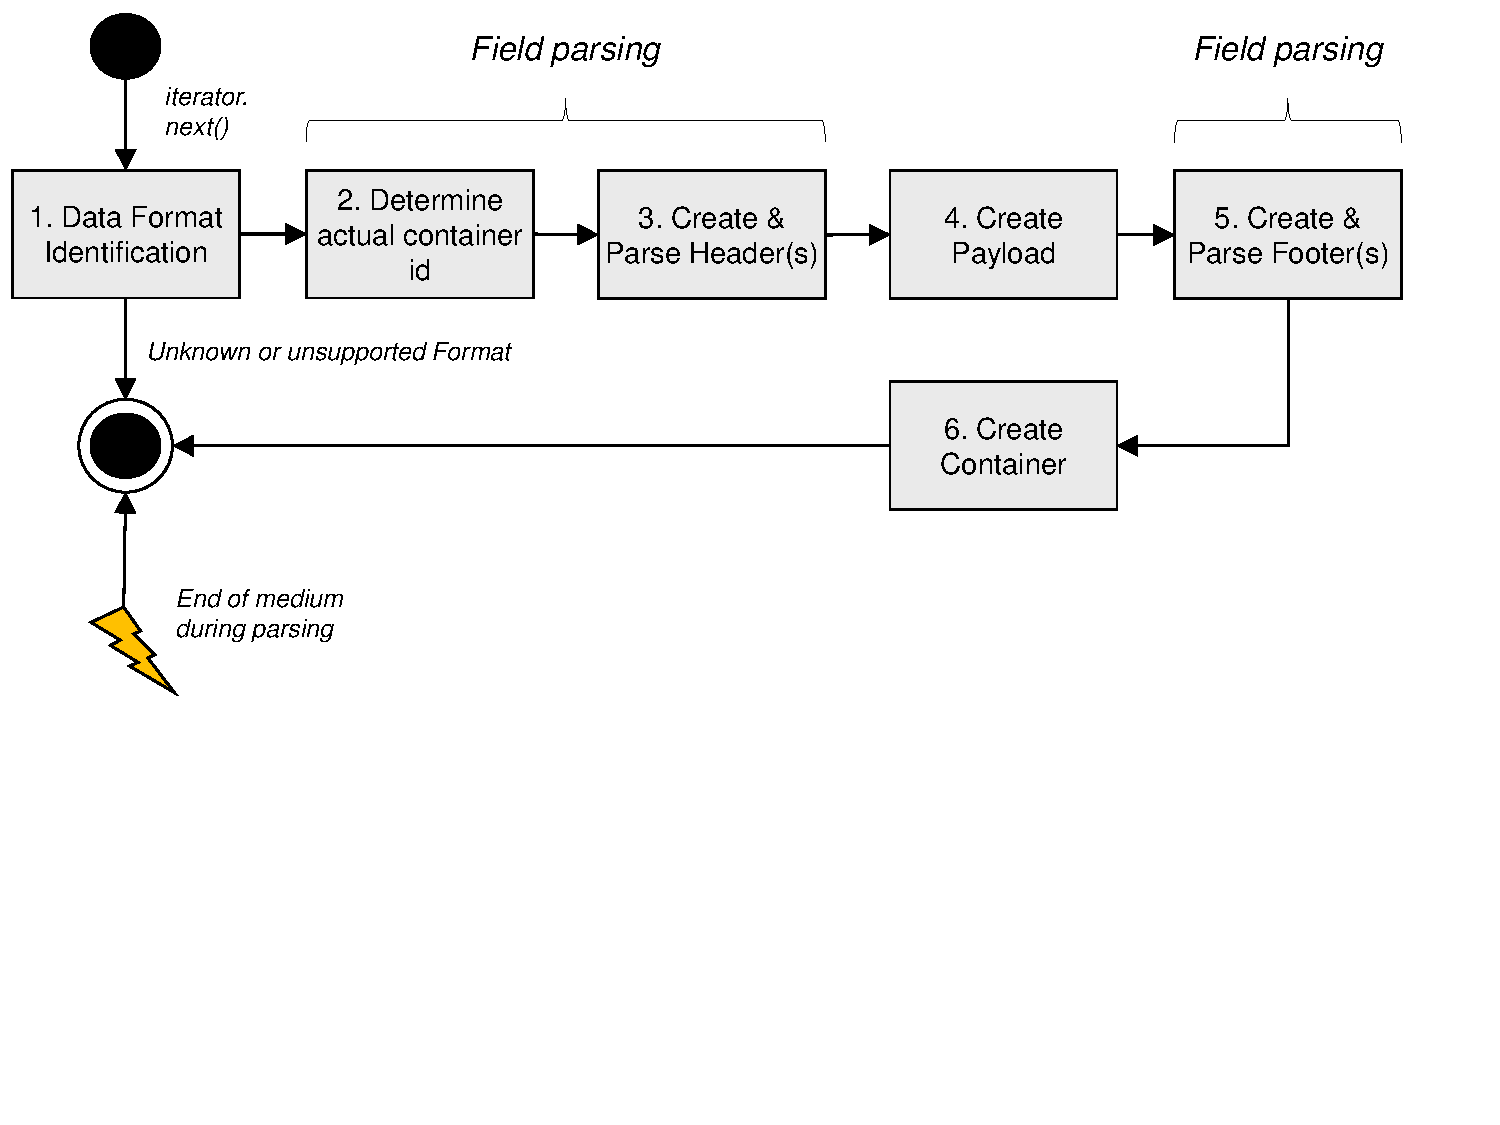
\includegraphics[width=1.0\linewidth]{figures/III_ForwardReading.pdf}
  \caption{Steps for reading data forward}
  \label{fig:III_ForwardReading}
\end{figure}

%%%% DD --> %%%%
\DD{dd:605}
{% Title
Steps of forward reading of top-level containers
}
{% Short description
  Forward reading of a single top-level container works as follows - whenever \texttt{next()} on the iterator is called to read the first or next container:
  \begin{enumerate}
  \item First, we do data format identification, i.e. finding out whether the data chunk ahead belongs to a data format the library supports - see \SectionLink{sec:MagicKeys} for details. If we cannot identify the data format, the process stops here with an exception.
  \item After identifying the data format, we need to identify which concrete container type and id we have, i.e. determining its structure and actual id at runtime; this is especially necessary for data formats supporting generic containers which is most of the container data formats out there, or multiple different container types. 
  \item Then, as we forward-read, the headers of the container are parsed, which means understanding their content. This includes determining if there are other headers or footers, and also the length of the container's payload.
  \item After heaving determined the payload length, the payload object itself is created. 
  \item Then, if there are any footers, they are at least created and ready to be parsed.
  \item Finally, the container is created which consists of the previously created headers, footers and payload
  \end{enumerate}
  It might happen that during this process, an expected or unexpected end of medium occurs. Expected it can only be during data format identification, in all other cases there seems to be a corruption in the data or parallel changes, as the parsing metadata indicates a size which is not matching reality.

  During steps 2, 3 and 5, fields need to be parsed which is a special discipline discussed later.
}
{% Rationale
The process is aligned at the structure of a container and typical for forward reading.
}
{% Disadvantages
No disadvantages known.
}
%%%% <-- DD %%%%

Btw:
%%%% DD --> %%%%
\DD{dd:605a}
{% Title
Steps of forward reading for nested containers
}
{% Short description
These are nearly identical except that data format identification is unnecessary.
}
{% Rationale
Nested containers are other than the fact that the data format is already known in no way different to top-level containers.
}
{% Disadvantages
No disadvantages known
}
%%%% <-- DD %%%%

% =======================================================================================================
\subsection{Buffering, Caching and Lazy Reading}%
\label{sec:ReadingSteps}%

\COMPdataPartManagement{} uses the features of \COMPmedia{} for caching as described in \SectionLink{sec:PerfMedia}. These features are also used for buffering, i.e.
%%%% DD --> %%%%
\DD{dd:606}
{% Title
General buffering using maximum read-write block size is done - for each overlap buffer the next block
}
{% Short description
  Most of the read operations in \COMPdataPartManagement{} do a buffering before accessing data. They always buffer at most maximum read-write block size of bytes. If a buffering call detects that the start offset of buffering plus maximum read-write block size exceeds current buffered data, it buffers the next block starting behind the currently buffered data with at most maximum read-write block size of bytes.

  This decision strongly bases on the critical design decision \DesLink{dd:438a} for a sensible handling of objects (e.g. fields) overlapping two consecutive byte blocks read.
}
{% Rationale
Reading byte by byte or field by field would be nonsense from performance point of view. The maximum read-write block size is a natural fit for buffering. The approach of buffering the next block when an overlap is detected is sensible as it leads to less cache fragmentation. The previously cached consecutive block will not fall out of the cache thanks to design decision \DesLink{dd:438a}.
}
{% Disadvantages
No disadvantages known.
}
%%%% <-- DD %%%%

Now the question arises: Where to buffer exactly to ensure that there is no ``buffer gap''?

%%%% DD --> %%%%
\DD{dd:606a}
{% Title
Buffering at start of container and field reading
}
{% Short description
  It turned out to be fully sufficient if we do the following:
  \begin{itemize}
  \item Buffer at start of container identification/reading: Whenever it is checked if a container with a given type and id during container identification phase is done, we first buffer read-write block size of bytes. As this size has a lower bound (see \DesLink{dd:438a}) with a sensible default, this way all usual headers are already buffered, leading to speeding up data format identification for top-level containers.
  \item Buffer at start of field reading: Whenever a single field of a header, footer or payload is read, buffering is done. Due to \DesLink{dd:606}, any overlapping bufferings will actually read the next block in addition, ensuring that always as sensible amount of future bytes is pre-buffered. This case also covers field based payload.
  \end{itemize}
}
{% Rationale
Thus, even if we have unusually long headers, footers or field-based payload, there is never a buffering gap.
}
{% Disadvantages
No disadvantages known
}
%%%% <-- DD %%%%

A very basic mechanism of container data formats is that they allow seeking and skipping based on containers, that means the decoders might just need to check a container header to find out if they are interested in the data it contains, and if not simply go on reading with the follow-up container. For this, most if not all data formats specify the size of the container in its header or footer. To fully support this, we define some kind of lazyness as follows:

%%%% DD --> %%%%
\DD{dd:607}
{% Title
Lazy payload
}
{% Short description
Any field-based or container-based payload is lazy by default, i.e. its bytes are first read only when explicitly requested by the user. A sole exception is in place for stream-based media (see upcoming design decision). 
}
{% Rationale
This way, we do not read unnecessary data the user might never look at, especially allowing to skip over large containers without risking out of memory and long read times, just perfectly meeting requirement \SectionLink{sec:REQ009LesenSchreibenGrosse}.
}
{% Disadvantages
No disadvantages known
}
%%%% <-- DD %%%%

As streams are non-random-access media, the question arises what we do with the bytes of a stream. It is no good idea to skip the payload byte here - what if the user wants to closely look at them? There is no other choice than to still cache them. The same is true for rather ``exotic'' formats such as Lyrics3v2 where the payload size is not contained in a header, but only in the footer.

%%%% DD --> %%%%
\DD{dd:608}
{% Title
Fully cache payload for stream-based media and formats without size field
}
{% Short description
  For stream-based media, the whole payload data must be fully read to at least have a chance that the user can look at it later. It might happen that the maximum cache size is exceeded in which case the first bytes of the payload might fall out of the cache.

For formats not having a static payload size and not having a size indicator in its header, the payload must be fully read in entirety to know its size. This also leads to potentially filling up the cache. 
}
{% Rationale
  There is no other way for streams than grabbing the bytes when looking at them - streams are just one time read.

  For the special case of formats not having a payload size in their header, see \DesLink{dd:529d}.
}
{% Disadvantages
No disadvantages known
}
%%%% <-- DD %%%%

% =======================================================================================================
\subsection{Container Context Information}%
\label{sec:ContainerContextInformation}%

In section \SectionLink{sec:FieldFunctions}, we already mentioned the \emph{parsing metadata} that is vital for understanding and reading a container. This information is tagged as such by each extension in the form of field functions that link fields to target blocks they refer to. This information is of course relevant for generically parsing a container at runtime. As soon as you encounter e.g. a field that contains the size of the container's payload during parsing, you have to store this size somewhere to be accessible later when actually parsing the payload.

Here, we summarize all the parsing metadata known at one point in time during container parsing as the \emph{container context information}. However, the container context information shall not only be a simple map storing the already known field functions, but it is intended to be more:

%%%% DD --> %%%%
\DD{dd:620}
{% Title
\texttt{ContainerContext} provides sizes, counts, byte orders and character encoding of all data blocks in a container; it is available in each data block; one instance per container
}
{% Short description
A helper class \texttt{ContainerContext} provides sizes, counts, byte orders and character encoding of \emph{all} data blocks in the current container. That means it not only stores the field functions refering to some of them, but also knows about static sizes, static occurrences, default byte orders and character encodings etc. It is an attribute of each data block such that it can be accessed from most places during as well as after parsing. The details of size determination are described in \SectionLink{sec:SizeDetermination}, the details of count determination in \SectionLink{sec:CountDetermination}.
}
{% Rationale
Having just one place that not only stores field function values but also knows in a more abstract way how to determine sizes, counts, byte orders and character encodings allows for better separation of concerns. This also allows to pass around corresponding objects to everywhere you need this information in contrast to having this logic only in a reader class that is not availabe anywhere else after parsing.
}
{% Disadvantages
No disadvantages known
}
%%%% <-- DD %%%%

One question that comes up here: How about parsing metadata available in the top-level container, but needed in a child container? We define:

%%%% DD --> %%%%
\DD{dd:621}
{% Title
\texttt{ContainerContext} contains a reference to the direct parent container's context and searches the parent for metadata if none is found in itself
}
{% Short description
\texttt{ContainerContext} contains a reference to the direct parent container's context (if any). If it cannot come up with a size, count, byte order or character encoding itself, it asks the parent for such metadata.
}
{% Rationale
This way, parsing metadata only defined in the top-level container headers can be transported to children deeper in the hierarchy.
}
{% Disadvantages
No disadvantages known
}
%%%% <-- DD %%%%

% -------------------------------------------------------------------------------------------------------
\subsubsection{Size Determination}%
\label{sec:SizeDetermination}%

How to determine the sizes of data blocks before parsing? It is clearly necessary to know the size of a container in advance to be able to parse or skip it. Unfortunately, all data formats seem to follow a distinct strategy of how to specify sizes as indicated around design decision \DesLink{dd:540}.

The cases we have to handle are summarized as follows:
%%%% DD --> %%%%
\DD{dd:640}
{% Title
Cases for size determination
}
{% Short description
  The easiest \textbf{Case 1:} Static size indicated in the specification. If a data block's specification indicates a static size, this size is taken during parsing.

  Otherwise, the data block has a dynamic size which breaks down to the following cases:
  \begin{enumerate}
  \item[\textbf{Case 2:}] The data block's size is directly indicated by another field that must be parsed before (usually in header or footer) - Note that this size might include the size of other blocks in addition, see \DesLink{dd:542} and the discussion around for more details. Here, ``directly'' means that the field is a numeric value greater or equal to the size, and we do not need to calculate something.
  \item[\textbf{Case 3:}] The data block's size is indirectly indicated by other fields that must be parsed before (usually in header or footer). ``Indirectly'' means that the field is not just single or summed size contained in a field, but there is a more complex calculation of combining multiple field values to calculate the size. This is e.g. the case for the size of the MP3 container payload or the Ogg page payload and packet part sizes.
  \item[\textbf{Case 4:}] The data block is payload consisting of fields or containers, and there is no size indicator at all. However, it is clear how to determine the sizes of all children of the payload block, and thus the size of it is the sum of the sizes of all its children. This is e.g. the case for Lyrics3v2 tag payload.  
  \item[\textbf{Case 5:}] The data block is a terminated field, i.e. its size must be determined by finding its termination. The handling of this case is defined in \SectionLink{sec:TerminatedFields}.
  \item[\textbf{Case 6:}] None of the other cases applies, but at least the overall remaining size of the parent data block is known. Take the remaining size of the parent data block as size of the data block.
  \end{enumerate}

  \LibName{} supports exactly those cases. Despite case 5, they are implemented in the \texttt{ContainerContext}, see \SectionLink{sec:ContainerContextInformation}.
}
{% Rationale
The cases come from analyzing different data formats \LibName{} is required to support, so it is sufficient to consider only those (if any others exist). Why is case 5 not implemented in \texttt{ContainerContext}? The reason is that finding termination bytes requires parsing itself, so it must be implemented in the reader.
}
{% Disadvantages
No disadvantages known
}
%%%% <-- DD %%%%

Case 1 is already clear how to deal with, case 5 is treated later in \SectionLink{sec:TerminatedFields}. Thus we are left to deal with cases 2 to 4. First of all, we consider case 3:

%%%% DD --> %%%%
\DD{dd:641}
{% Title
Complex size calculation from fields done in custom implementation via \texttt{SizeProvider}
}
{% Short description
Data format extensions are allowed to register a custom \texttt{SizeProvider} implementation which calculates the size of a data block as required by the format. This is used for Ogg, ID3v2.3 extended header size and MP3.
}
{% Rationale
More flexibility also for yet other future formats.
}
{% Disadvantages
No disadvantages known
}
%%%% <-- DD %%%%

Case 4 is handled as follows:
%%%% DD --> %%%%
\DD{dd:642}
{% Title
Determine payload size by reading all children
}
{% Short description
In case 4 of \DesLink{dd:640}, the size of the payload is calculated by reading all children, may it be containers or fields, and summing up their sizes. If at least one of their sizes could not be determined, this is a runtime exception.
}
{% Rationale
Straightforward and not too complex in terms of ``lazyness''. If the data formats design is fucked up, the implementation cannot easily work around it.
}
{% Disadvantages
No disadvantages known
}
%%%% <-- DD %%%%

Now we have case 2 left. This one is adressed with using field functions - potentially referring to multiple consecutive blocks as indicated by \DesLink{dd:540}. We clarify how it works by summing up the whole progress of size determination in total:

%%%% DD --> %%%%
\DD{dd:644}
{% Title
Size determination process
}
{% Short description
  Whenever the size of a single data block needs to be determined, the following steps are performed in the given order of precedence:
\begin{enumerate}
\item (Outside of \texttt{ContainerContext}) If the data block is a terminated field without fixed size, search for the termination character (case 5)
\item Otherwise if the current data format has a registered \texttt{SizeProvider} (see \DesLink{dd:641}), first ask this instance if it can provide a defined size (includes also case 3)
\item Otherwise if the data block has a static size according to its specification, take this size (case 1)
\item Otherwise if the current \texttt{ContainerContext} has a \texttt{SizeOf} field function, take the size indicated by the \texttt{SizeOf} field (part 1 of case 2)
\item Otherwise if the current \texttt{ContainerContext} has a \texttt{SummedSizeOf} field function for multiple data blocks and the sizes of all other blocks are known, take the \texttt{SummedSizeOf} field's value minus the summed size of the other data blocks (part 2 of case 2) - How to avoid an infinite loop here? This has been treated in design decision \DesLink{dd:541} and is also discussed with an example after this design decision.
\item Otherwise if the data block is a concrete data block that is derived from a generic data block, it is checked if there is a known size for the generic id  
\item Otherwise if the parent \texttt{ContainerContext} has a \texttt{SizeOf} field for it, take the size of the parent \texttt{ContainerContext}
\item Otherwise if the data block is a field or payload and the remaining parent size is known, take the remaining direct parent size as its size (case 6)
\item (Outside of \texttt{ContainerContext}) Otherwise if the data block is a payload block, read all its children and sum up their sizes (case 4)
\end{enumerate}
}
{% Rationale
The order of steps clearly focusses on least complexity first and tries to avoid unnecessary lookups by first considering fixed sizes and custom size providers.
}
{% Disadvantages
No disadvantages known
}
%%%% <-- DD %%%%

Some subtle point in determining sizes of single data blocks whose \texttt{SummedSizeOf} field is the sum of multiple consecutive data blocks is: If we want to determine the size of a single one, we have to determine the size of all the others, sum this size and subtract it from the value stored in the \texttt{SummedSizeOf} field. If for some stupid reason there are multiple data blocks included with a dynamic size, this could end up in an infinite loop such as for ID3v2.3: Size of payload needs to be determined, thus determine the size of the extended header first. However, the size of the extended header is also dynamic. The implementation would see that it would need the size of the payload to calculate the size of the extended header and thus call the first function again... To avoid this crap, we already stated the validity criteria in \DesLink{dd:541}.

% -------------------------------------------------------------------------------------------------------
\subsubsection{Count Determination}%
\label{sec:CountDetermination}%

Here we discuss how the determination of the number of occurrences of a data block (i.e. count determination) works. First of all, we can state that the number of payload containers is always 1, so no need to consider this case. For all other types of data blocks, there can be 0 to multiple occurrences.

The process to handle is summarized as follows:

%%%% DD --> %%%%
\DD{dd:645}
{% Title
Count determination process
}
{% Short description
  Whenever the count of a single data block needs to be determined, the following steps are performed in the given order of precedence:
\begin{enumerate}
\item If the current data format has a registered \texttt{CountProvider}, first ask this instance if it can provide a defined size
\item Otherwise if the data block has a static number of occurrences according to its specification, take this count
\item Otherwise if the data block is optional, i.e. either is present once or not at all, and if the current \texttt{ContainerContext} has a \texttt{PresenceOf} field function, take 1 as count if its presence is indicated by the flags, 0 otherwise
\item Otherwise if the current \texttt{ContainerContext} has a \texttt{CountOf} field function, take the count indicated by the \texttt{CountOf} field
\item Otherwise if the parent \texttt{ContainerContext} has a \texttt{CountOf} field for it, take the size of the parent \texttt{ContainerContext}
\end{enumerate}
}
{% Rationale
The order of steps clearly focusses on least complexity first and tries to avoid unnecessary lookups by first considering fixed counts and custom count providers.
}
{% Disadvantages
No disadvantages known
}
%%%% <-- DD %%%%

% =======================================================================================================
\subsection{Field Parsing}%
\label{sec:FieldParsing}%

Field parsing is the most complex part of reading data format bytes. It requires answers to following questions:
\begin{itemize}
\item How to determine the size of the field? - This has been answered already in \SectionLink{sec:SizeDetermination}, except the case of terminated fields which we treat here
\item How to determine the number of occurrences of a field, especially the case of optional fields? - This has been answered already in \SectionLink{sec:CountDetermination}
\item Which byte order (for numeric fields) and character encoding (for string or enumerated fields) needs to be used when? - This has been answered already in \SectionLink{sec:ContainerContextInformation}
\item How to convert the binary field value to an interpreted one?
\item How to use caching during field parsing?
\end{itemize}

% -------------------------------------------------------------------------------------------------------
\subsubsection{Terminated Fields}%
\label{sec:TerminatedFields}%

Terminated fields are those fields with a dynamic length that is not given by the value of another field, but these fields are delimited by a sequence of termination bytes or characters. 

Terminated fields are worst-case for parsing: First of all you never know when it ends, and second you have to deal with strings which brings different encodings into play.

Let's deal with the first problem, the unknown length. Of course, in the ``usual'' case a terminated field is still a field and thus relatively small. We will only rarely encounter terminated fields longer than several KB. In order to be fully generic, one needs to deal with the worst case of fields having up to \texttt{Long.MAX\_VALUE-1} as size. Having said this, also block-wise reading is required as we do not want to risk out-of-memory conditions by soaking too much bytes into memory. One could come up with the idea of using some upper bounds for reading data, i.e.:
\begin{itemize}
\item \textbf{Case 1:} The current total medium size as well as the exact size of a parent of the field is known - E.g. for ID3v23 text frames, the frame size and thus payload size is known, but there is a terminated text payload field; for file and byte array media, the medium length is also known.
\item \textbf{Case 2:} The current total medium size is unknown, yet the exact size of a parent of the field is known - Take an ID3v23 text frame on an input stream medium as an example.
\item \textbf{Case 3:} The current total medium size is known, but the exact size of a parent of the field is unknown - Take an APEv2 item header on a file or byte array medium as an example. Here, the item key is terminated, and the size of the parent header is unknown as it is only determined by the sum of the field sizes and not - in addition - by any size indicators.
\item \textbf{Case 4:} Neither current total medium size nor the exact size of a parent of the field is known - So APEv2 item header on an input stream medium is an example.
\end{itemize}

%%%% DD --> %%%%
\DD{dd:650a}
{% Title
Block-wise reading for finding field termination
}
{% Short description
Block-wise reading is necessary in order to find field termination. According to \DesLink{dd:438}, we do not read more than the configured maximum read-write block size in bytes from the medium at once. Actually, we \emph{always} read the configured maximum read-write block size and do not take into consideration any additionally known upper bounds such as the remaining parent byte count or remaining medium length (if available). If an end of medium is encountered during reading a block of data, we scan for the termination within the actually read bytes. Otherwise the next block is read for scanning for termination bytes and so on. However, we can at least take into account any available bounds for finding out if we need to search further or we can skip the process: If the already read byte count is bigger than the remaining parent byte count, we should skip as a data corruption might be present.
}
{% Rationale
Block-wise reading avoids out-of-memory conditions and is a compromise between reading too much and reading too few bytes at once. Of course this compromise comes with the cost of added complexity. We mitigate this complexity by not coming up with further ``optimizations'' such as only reading up to a known upper bound like the medium end or parent end. In the end, both might not be known, especially in case 4, thus anyway we have to do a ``blind'' reading in this case.
}
{% Disadvantages
Added complexity, but in conformance with \DesLink{dd:438}. The complexity is adressed as specified in the rationale.
}
%%%% <-- DD %%%%

Regarding strings and their encoding: First of all, we remember that only string and string list fields can be terminated and thus it is fine to talk about \emph{termination characters} instead of termination bytes (see \DesLink{dd:531} and \DesLink{dd:532}). How should we parse terminated fields to detect the termination character? We could do it either:
\begin{enumerate}
\item by converting the character to a byte sequence and then searching the termination
\item by converting the bytes to a string and then trying to find the termination character or
\end{enumerate}

Both approaches have their serious drawbacks. \textbf{Approach (1)} requires us to know where a character starts and ends such that we can correctly match termination bytes only at character borders. For instance UTF-16 encodes all characters always as two bytes. It would be wrong to try to detect termination bytes at odd offsets. Instead we have to ensure to search for them only at even offsets.

\textbf{Approach (2)} suffers from a similar problem that there is no nice way to handle block-wise split strings: If we read block-wise, it might be that a single character spanning multiple bytes is just torn apart at a block border. E.g. UTF-8 is a variable length encoding where - depending on the first byte - the total number of bytes of a character is given. If a converter from byte to string encounters a torn apart character at the end of the byte sequence, it might fail with some kind of decoding runtime error, so we have to handle this separately. However, Java's \texttt{CharsetDecoder} seems just about right for this task. ID3v2.4 supports UTF-16LE, UTF-16BE, ISO-8859-1 as well as UTF-8 so we have to handle such cases.

We define:
%%%% DD --> %%%%
\DD{dd:650}
{% Title
Character-based termination detection
}
{% Short description
We use character-based termination detection (approach 2) for finding termination characters and do not use termination-byte-based detection (approach 1)
}
{% Rationale
This is possible due to the fact that only string and string list fields can be terminated (see \DesLink{dd:531} and \DesLink{dd:532}). Approach 1 seems even harder as we need to re-implement parsing of strange encodings while approach 2 at least provides an out-of-the box solution in the form of  \texttt{CharsetDecoder}.
}
{% Disadvantages
No disadvantages known
}
%%%% <-- DD %%%%

No we can summarize the process of finding termination of a field:
%%%% DD --> %%%%
\DD{dd:651}
{% Title
Determining the end of a terminated field
}
{% Short description
  As input for the algorithm, we get the current medium offset, the character encoding of the bytes as well as the termination character to find and the maximum read-write block size. The steps are as follows:
  \begin{enumerate}
  \item Read $N:=$ read-write block size bytes from the medium at the current offset
  \item If end of medium occurs, take the actually read bytes and mark the algorithm for termination as no further input is available
  \item Search the input buffer for the termination character by actually decoding bytes according to the character encoding using \texttt{CharsetDecoder}
  \item If there should be a character overlapping a block border, use the facilities of \texttt{CharsetDecoder} to overcome the situation
  \item If a termination character is found, mark the algorithm for termination
  \item Otherwise:
    \begin{enumerate}
    \item If the remaining parent byte count is known and the already read byte count is bigger than this value, mark the algorithm for termination 
    \item Otherwise increment the current medium offset by the maximum read-write block size and goto step 1
    \end{enumerate}
  \end{enumerate}
}
{% Rationale
This process is efficient in terms of avoiding unknown steps and using only sparse memory. It is as simple as it can get without risking incorrectness.
}
{% Disadvantages
No disadvantages known
}
%%%% <-- DD %%%%

% -------------------------------------------------------------------------------------------------------
\subsubsection{Lazy Fields}%
\label{sec:LazyFields}%

In this section, we want to investigate if we need a kind of lazy field (similar to lazy payload as described in \DesLink{dd:607}). The idea: What if a field is large and we know this in advance? Should we read all field bytes into memory or rather not?

First of all, we shall check if there are cases that clearly come to mind here:
\begin{itemize}
\item Ogg contains segments within its payload that only get a max size of 255, so no need here for lazy fields; also the ogg header is quite harmless
\item APEv2, Lyrics3v2, ID3v1 and ID3v2 only define small fields
\item MP3 payload fields might not be longer than 998 bytes, so no lazyness required here
\item RIFF, QuickTime and Matroska might have arbitrary large payload, and thus arbitrary large fields to read
\end{itemize}

Thus, considering the formats, we already see that large fields might occur. So we define:

%%%% DD --> %%%%
\DD{dd:652}
{% Title
Lazy fields in case field size is known and exceeds the maximum read-write block size 
}
{% Short description
A special case for large fields is introduced: If the field size is known in advance (i.e. is either static or given by field function or remaining parent size) and is bigger than the maximum read-write block size, the field is created as lazy field and its bytes are only first read when explicitly requested by the user.
}
{% Rationale
This avoids unwanted out-of-memory conditions. Terminated fields, where field size is not known in advance, need not be lazy, as when determining their size, they are anyway read into memory.
}
{% Disadvantages
Slight increase in complexity
}
%%%% <-- DD %%%%

% =======================================================================================================
\subsection{Backward Reading}%
\label{sec:BackwardReading}%

The feature of reading backward is just a convenience and performance improvement functionality. It has a lot of differences compared to forward reading, i.e. it is not only just ``reversed forward reading''. The reason is that APIs do not know some kind of ``backward read mode'', i.e. file I/O and array APIs only allow to read forward starting at offset $x$. The problem with this is that you do not know where $x$ is during backward reading, because e.g. $x$ is the starting point of a dynamic length data block, but you are currently positioned at its end and have no idea where it starts.

Nevertheless, some data formats support backward reading by providing a so-called footer. The reason for this feature is that multimedia files are easier to modify at their end than at the beginning: Wen inserting a tag of length $n$ at the beginning of the file, you actually have to read all bytes of the file, write them to offsets $x+n$, and then write the tag bytes at offset 0. This requires a lot of I/O and can be expensive, especially for large files. Appending tags at the end of file avoids this. To ensure that parsers can identify such end-of-file tags, footers have to be defined and present. From the supported formats, Lyrics3v2, ID3v2.4 and APEv2 support footers. ID3v1 can be read backwards, too, as it is of static length.

However, first of all, we have to note down:
%%%% DD --> %%%%
\DD{dd:653}
{% Title
Streaming media cannot be read backwards
}
{% Short description
\LibName{} cannot read stream-based media backwards and reacts with a runtime exception if a user tries to do that
}
{% Rationale
Random access media allow starting reading from any point, streams by design do only start at the beginning.
}
{% Disadvantages
No disadvantages known
}
%%%% <-- DD %%%%

If we do backward reading, the first question that might come up is: How do we actually do it? Quite similar to forward reading but with some important differences:
%%%% DD --> %%%%
\DD{dd:654}
{% Title
Backward reading uses footer magic keys
}
{% Short description
When backward reading, \COMPdataPartManagement{} tries to find a footer magic key at a fixed position in front of the current offset. If it can find it there, this is a signal that a container of the given data format is present. The implementation tries to extract a static payload size from the footer(s). Then it reads the payload using this static size by going that much bytes backward. Finally, it reads any header(s) in front. If start of medium is encountered during this, this is quite similar to an end of medium unexpected error.
}
{% Rationale
This allows to reuse some parts of forward-reading and thus avoids to invent something totally different.
}
{% Disadvantages
No disadvantages known
}
%%%% <-- DD %%%%

\DesLink{dd:654} did mention a basic approach and also footer(s) and header(s). But how to deal with dynamic length headers or footers or unknown length payload? The problem here is that you only know where a footer, payload or header ends, but not where it actually starts if it is dynamic or unknown length. For now, we state:

%%%% DD --> %%%%
\DD{dd:655}
{% Title
Only static length headers, payload and footers are supported for backward-reading
}
{% Short description
As of the current release, \LibName{} cannot deal with dynamic length headers or footers during backward reading. It throws a runtime exception if the presence of such a dynamic-length header is detected. The same is done if the lenght of payload could not be determined. However, \LibName{} fully supports multiple static-length headers or footers as well as optional ones, with quite the same mechanisms as for forward-reading. 
}
{% Rationale
This is e.g. the case for ID3v2.4: If there is an extended header (which has dynamic length) there is no way to find out where it starts during backward reading except you search for the actual main header starting point. This would somehow not exactly fit with the forward-read approach. There is an option to implement it later or for the extensions to overwrite the default implementation in a more flexible way.
}
{% Disadvantages
No disadvantages known
}
%%%% <-- DD %%%%

One observation that is important to grasp comes when you think about parsing the content of a container that has already been backward-read:

%%%% DD --> %%%%
\DD{dd:656}
{% Title
Payload content of a backward-read container is forward-read
}
{% Short description
As soon as we have fully read a container backwards, we of cause know where its payload starts and ends. Thus, we can of course read the payload \emph{forward} instead of backward. The same is of course true for headers and footers during backward-reading: As we know where they start, we wouldn't want to read their fields somehow backwards. Instead we simply reuse the existing code that forward-reads fields.
}
{% Rationale
We can reuse a lot of code for forward-reading instead of coming up with new code. Decreases complexity.
}
{% Disadvantages
No disadvantages known
}
%%%% <-- DD %%%%

Finally, we look at a special case of backward reading: ID3v1.

%%%% DD --> %%%%
\DD{dd:657}
{% Title
ID3v1 can be backward-read as it is static size, this is done in the extension
}
{% Short description
As ID3v1 has a static size of 128 bytes, we can always check if there is the header's magic key at -128 bytes from the current offset. If so, we've found the tag during backward reading. However, as ID3v1 does not have a footer but only a header, this special case has to be implemented in a custom implementation of the extension and not in the generic centralized code.
}
{% Rationale
ID3v1 frequently occurs at the end of a medium and thus it makes sense to support this.
}
{% Disadvantages
No disadvantages known
}
%%%% <-- DD %%%%

% =======================================================================================================
\subsection{Basic Concept for Writing}%
\label{sec:BasicConceptforWriting}%

Here, we care about the basics for writing. Writing data is an intgral part of the \COMPdataPartManagement{} component. The question is: How can a user manipulate data? What is already clear is that we cannot write to stream-based media and the attempt will lead to a runtime exception (see \SectionLink{sec:ZugriffEinesTERMmedium}).

What can be already noted is that we will of course use the features of \COMPmedia{}:
%%%% DD --> %%%%
\DD{dd:660}
{% Title
Using \COMPmedia{} with two-staged write protocol
}
{% Short description
\COMPdataPartManagement{} uses the \COMPmedia{} API to perform the writing. Thus, it also has to adhere to the two-stage write protocol as described in \SectionLink{sec:GrundSchreiben}. That means that first, changes are done as needed, and then the user needs to perform an actual flush of the changes in a second step. For read-only media, an exception is thrown only when trying to flush changes.
}
{% Rationale
Otherwise we needn't do the fuss in \COMPmedia{}. Two-stage writing is sensible as usually one change is not done isolated but leads to a series of other changes. The user can safely do the changes and then ``commit'' at a sensible time, leading to even a better performance.
}
{% Disadvantages
No disadvantages known
}
%%%% <-- DD %%%%

However, if we do it like that, one question immediately arises: What does the user ``see'' after having done changes but not yet having flushed them? For instance, the user may add an extended header to an ID3v2.3 tag or remove a frame from it. If the user then iterates the frames, will the removed frame still be returned or not? 

%%%% DD --> %%%%
\DD{dd:661}
{% Title
The user sees the dirty state of the containers when calling read methods
}
{% Short description
Once the user has done changes on a \IMediumStore{} using the writing API of \COMPdataPartManagement{}, these changes will be visible and active in the reading API of \COMPdataPartManagement{}, even if they are not yet flushed. Removed blocks won't be returned anymore, inserted blocks will be returned, and changed field values will also be returned. The user would not see these changes using another \IMediumStore{} to access the medium. However, this is not possible due to the locking concept of \COMPmedia{}.
}
{% Rationale
  This seems to entirely contradict with \DesLink{dd:410c} that states: \COMPmedia{} read methods always return the currently persisted state. However, the written data is still available in terms of added data blocks.
  
It would be quite strange for the user if data blocks previously inserted would not be returned again when reiterating the blocks. This could cause confusion for the users and would e.g. not offer the possibility to undo changes if the user did not keep a reference to an insterted block.
}
{% Disadvantages
No disadvantages known
}
%%%% <-- DD %%%%

In section \SectionLink{sec:FieldFunctions} we introduced the so-called field functions as a way to indicate dependencies between fields and other data blocks. However, just modeling this dependency without using it in anyway is of course nonsense. The main driver for introducing this concept is consistency: If you have a size field indicating the size of payload, and if that payload changes, we want the size field to change consistently without manual intervention of the user. Thus, we have to implement this feature during writing. This goes hand in hand with the two-stage write protocol decided in \DesLink{dd:660}.

%%%% DD --> %%%%
\DD{dd:662}
{% Title
Fields with functions are consistently updated during writing 
}
{% Short description
Whenever a user changes a datablock that is referenced by another field with a field function, the field's value must be updated according to the kind of change: \texttt{SizeOf}, \texttt{SummedSizeOf}, \texttt{CountOf} and \texttt{PresenceOf} are updated once a user writes to data blocks these field functions refer to. The fields themselves need to be read-only to ensure consistency. On the other hand, \texttt{CharacterEncodingOf} and \texttt{ByteOrderOf} fields can be written, leading to an inverse change to all data blocks they refer to: If you change the fields value, the byte order or character encodings of the target data blocks must change automatically, leading to a potential change to any numeric or string target fields. The two-stage write protocol of \DesLink{dd:660} minimizes the chance that there is an inconsistent state where the field value changes but not the referred data blocks, because the change is first getting only scheduled consistently, and later written in a ``single'' operation. 
}
{% Rationale
Consistency and user convenience
}
{% Disadvantages
Of course this makes the implementation more complex and in the first place requires the concept of field functions.
}
%%%% <-- DD %%%%

A second inference from using a two-stage write protocol is the possibility of a ``rollback'' - which MUST not be confused with ACID in any way:
%%%% DD --> %%%%
\DD{dd:663}
{% Title
Undo possibilities of unflushed changes are necessary
}
{% Short description
It needs to be necessary that the user can undo all changes he has done before a flush. However, it must be clearly communicated in the API and documentation that this whole thing is in no way ACID! Thus we do not actually call it ``rollback''. Flushing changes can go wrong in the middle, leaving part of the changes already written to the medium. Likewise, ``rollback'' could fail in between, but will at least not messing up the medium, as nothing has been written yet. See \DesLink{dd:410b} for further details.
}
{% Rationale
If having a two-stage write protocol, this desire comes to mind. If I can mark something for change, why can I not undo it? The second thing is field functions (\DesLink{dd:662}): If we change fields according to other changes, then being able to undo these connected changes also in a consistent way is necessary. Another argument is that we have some possibility to do that in the undo functionalities of \COMPmedia{}, see \DesLink{dd:420}.
}
{% Disadvantages
Implementing this of course requires some effort: You need to ensure that every change is properly undone.
}
%%%% <-- DD %%%%

Having talked about consistency, it comes to mind: Whenever a user changes something or creates something new, there are a myriad of possibilities why this change is utterly against the data formatt's specification. A field value could be invalid, the size of something could be too big or small, the type or structure of the thing to add could be tried to be added at the complete wrong place etc. How do we deal with such things?

%%%% DD --> %%%%
\DD{dd:662}
{% Title
Strict validation of specification conformance as early as possible
}
{% Short description
For every writing action, \COMPdataPartManagement{} strictly checks the validity of the things done against the data format specification. If the change violates properties of the data block changed or its parent, this is clearly and directly communicated with a runtime exception. The details are defined in later individual design decisions.
}
{% Rationale
Fail fast is a good principle, here even more. We want to avoid the user to write any crap to the medium that cannot be re-read, as it might be utter nonsense.
}
{% Disadvantes
No disadvantages known
}
%%%% <-- DD %%%%

Already now, it clearly emerges that the writing API will be fundamentally different from the reading API:
%%%% DD --> %%%%
\DD{dd:663}
{% Title
Writing methods are scattered in the API in contrast to reading
}
{% Short description
There is a fundamental asymmetry between reading and writing: While reading is done using an iterator approach and a core class that does the reading, writing is done by methods associated with the datablocks themselves. For extensibility this means that there is no single class the user can subclass to extend the writing functionality.
}
{% Rationale
Reading is done step by step at once in a linear process, while writing means to manipulate the individual objects that have previously been read or created.
}
{% Disadvantages
Writing is harder to extend, but currently there seems to be no need to do so
}
%%%% <-- DD %%%%

% =======================================================================================================
\subsection{The State of a Datablock}%
\label{sec:StatesofDatablocks}%

If \LibName{} would only support reading of datablocks, a datablock state would probably not be necessary. However, if datablocks are modified and as we have a two-stage write protocol, states become indeed a necessity, as actions depend on the current state of a datablock. We can think of the following states:
\begin{longtable}{|p{0.15\textwidth}|p{0.8\textwidth}|} \hline
  \textbf{State} & \textbf{Description} \\ \endhead \hline
  \texttt{NEW} & The datablock has been newly created or persistently removed from the medium. That means it is not attached to a parent datblock and does not have an offset. \\
  \hline
  \texttt{PERSISTED} & The datablock is persisted on a medium and thus has an offset. There are no modifications in the datablock that are not yet flushed. This is the state of a datablock after reading. \\
  \hline
  \texttt{INSERTED} & The datablock has been newly inserted into the medium and attached to a parent, but this change was not yet flushed. \\
  \hline
  \texttt{REMOVED} & The datablock has been removed from the medium and detached from a parent, but this change was not yet flushed. \\
  \hline
  \texttt{MODIFIED} & The datablock has been modified, but this change was not yet flushed. \\
  \hline
  \caption{Datablock states}
  \label{tab:Datablockstates}
\end{longtable}

%%%% DD --> %%%%
\DD{dd:670}
{% Title
A datablock in \LibName{} has one of the states listed in table \ref{tab:Datablockstates}.
}
{% Short description
A datablock in \LibName{} has one of the states listed in table \ref{tab:Datablockstates}.
}
{% Rationale
Depending on the state, some actions are legal or illegal, or need to be performed differently. Further on, the user must have transparency what has been done with a block so far, so the state is a good indication. Other states than the ones mentioned are not required. A separate \texttt{MODIFIED} is needed due to fields whose values can be changed.
}
{% Disadvantes
No disadvantages known
}
%%%% <-- DD %%%%

The questions remaining now are: How do states exactly change? And what about the hierarchical dependencies between datablocks? The latter question needs to be investigated first. What if a parent of a datablock is removed, does state of the child change correspondingly?

%%%% DD --> %%%%
\DD{dd:671}
{% Title
If a datablock changes state, all its descendant blocks change to the same state
}
{% Short description
Any change to a datablock leads to the same state change in all its children and further descendants.
}
{% Rationale
Obviously, all descendants are contained within the bounds of the datablock. So if it becomes \texttt{NEW}, \texttt{PERSISTED}, \texttt{INSERTED}, \texttt{REMOVED} or \texttt{MODIFIED}, all its descendants also do.
}
{% Disadvantes
No disadvantages known
}
%%%% <-- DD %%%%

What about a change in a child or other descendant, does it have any effect on its parent?
%%%% DD --> %%%%
\DD{dd:672}
{% Title
Modification, insertion or removal of a descendant leads to all its parents transitioning to \texttt{MODIFIED} state  
}
{% Short description
A datablock changes into the \texttt{MODIFIED} state once any of its descendants are modified, inserted or removed.
}
{% Rationale
A change in any child leads to an actual change of data contained in the datablock. It would be misleading if the API would still say the datablock is \texttt{PERSISTED}, no matter there are unflushed changes in a child. Furthermore, implementing things such as flushing or undo will probably be easier if you can tell which top-level data blocks were modified in some way instead of needing to search all children until the leaf nodes of the hierarchy to find out.
}
{% Disadvantes
No disadvantages known
}
%%%% <-- DD %%%%

Now we have all ingredients to come up with a suitable state transition diagram, without actual method calls yet, see figure \ref{fig:III_DBStates.pdf}.

\begin{figure}[htbp]
  \centering
  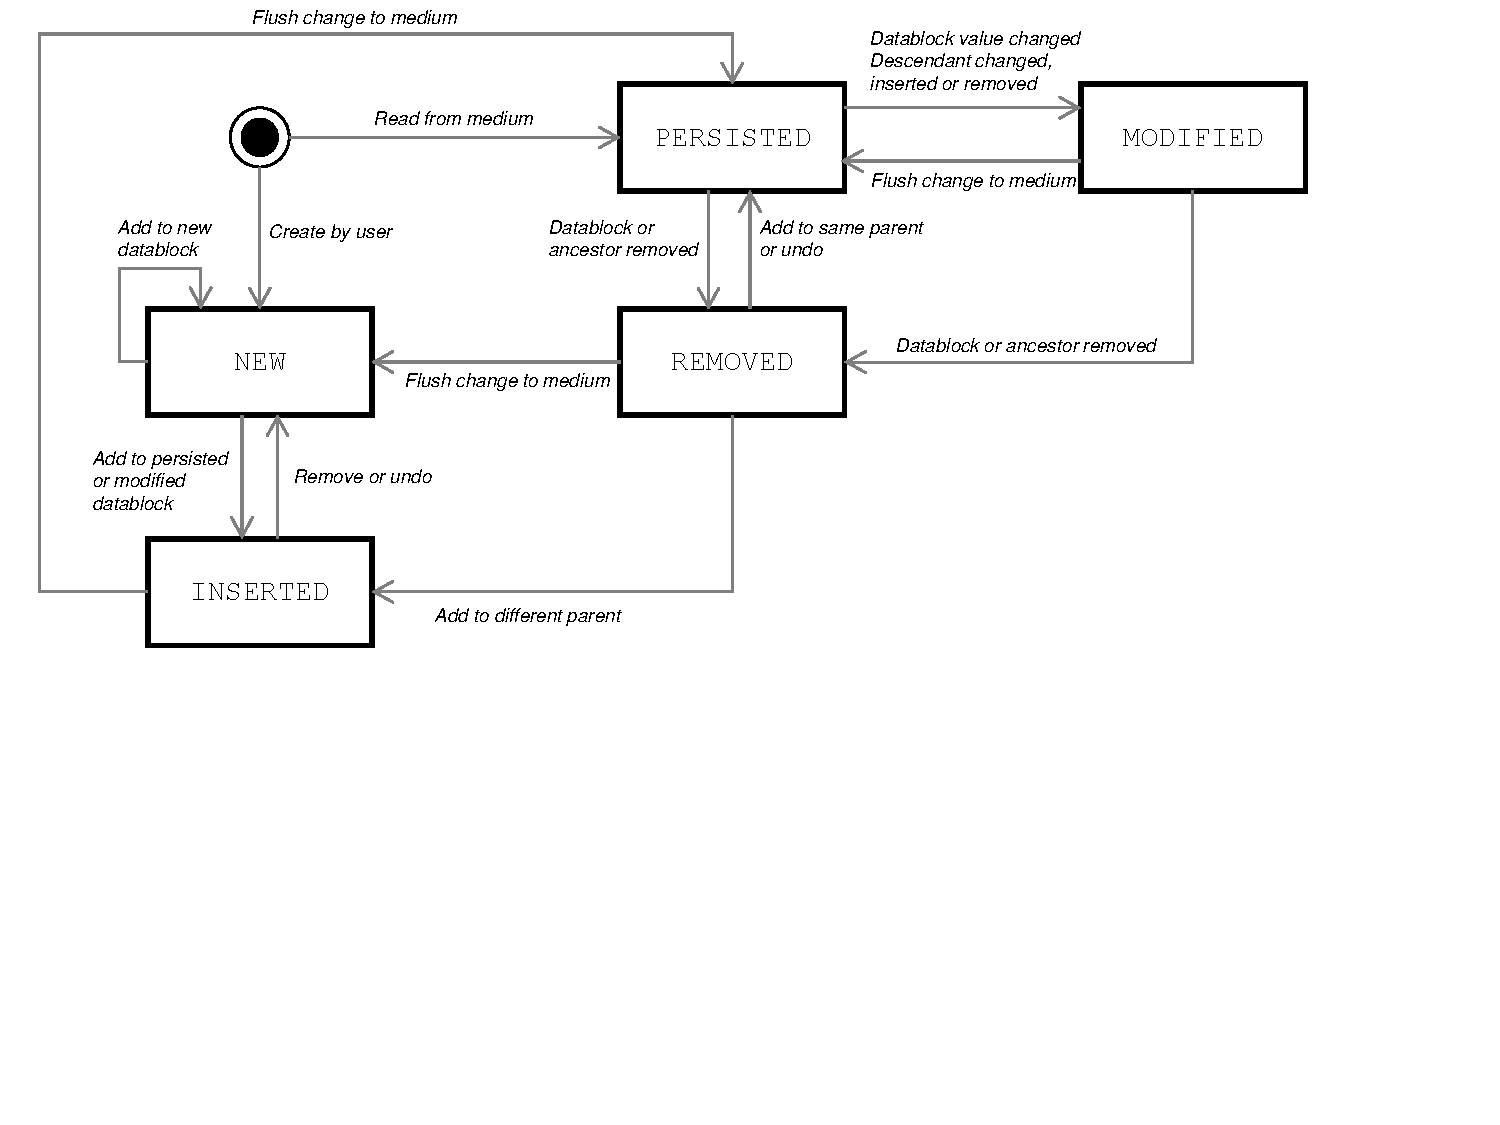
\includegraphics[width=1.0\linewidth]{figures/III_DBStates.pdf}
  \caption{Datablock state transitions}
  \label{fig:III_DBStates.pdf}
\end{figure}

% =======================================================================================================
\subsection{Writing Actions}%
\label{sec:WritingActions}%

In this section, we clarify in detail which write actions there are and how they need to work.

% -------------------------------------------------------------------------------------------------------
\subsubsection{Creating New Data blocks}%
\label{sec:CreatingNewDatablocks}%

First of all, in order to insert new data blocks, the user must be able to create new data blocks. The natural place to go is a factory:
%%%% DD --> %%%%
\DD{dd:675}
{% Title
A factory to create new data blocks
}
{% Short description
A factory instance accessible by the user is required to create new instances of containers, fields, headers, footers or payload. The created data blocks have the state \texttt{NEW}. The user specifies the id of the data block to create. The factory ensures that the given id belongs to the expected data format and has the correct type. Further validations are only done during insertion only. Of course for the user being able to specify an id during creation, every id must be publicly available in the API of the data format extension.
}
{% Rationale
A factory is a class that can create a family of products. This is clearly the case for data blocks. Different implementations can be created in future, if necessary. There is no direct dependency from user code to concrete data block classes. Some validations are done here already according to \DesLink{dd:662}.
}
{% Disadvantes
No disadvantages known
}
%%%% <-- DD %%%%

% -------------------------------------------------------------------------------------------------------
\subsubsection{Inserting Datablocks}%
\label{sec:InsertingDatablocks}%

\texttt{NEW} datablocks are inserted in their parent or at the top-level of the medium, respectively:
%%%% DD --> %%%%
\DD{dd:676}
{% Title
Insert methods for headers, footers and fields in their parent data block
}
{% Short description
To insert new headers, footers or fields, there are corresponding insert methods that do the job in the corresponding datablock class. They take an index that must be valid.
}
{% Rationale
You anyway need to have the parent instance, thus it makes sense to perform insertion in the parent itself, as the children are also anyway part of the parent.
}
{% Disadvantages
No disadvantages known
}
%%%% <-- DD %%%%

%%%% DD --> %%%%
\DD{dd:677}
{% Title
Insert methods for containers in container iterators
}
{% Short description
For both top-level as well as payload container iterators, there is an insert method in the iterator inserting a new container before the next container. That means to insert at a specific position, users first need to iterate to it. Containers can be inserted/appended at the end of the medium as soon as hasNext returns false. 
}
{% Rationale
This is quite similar to the insertion of headers, footers and fields.
}
{% Disadvantages
No disadvantages known
}
%%%% <-- DD %%%%

Now what about payload datablocks? For these insert methods wouldn't make much sense. Thus we define:
%%%% DD --> %%%%
\DD{dd:678}
{% Title
Simple setter method for payload datablocks
}
{% Short description
Payload children can be set with a setter method
}
{% Rationale
There is always just exactly one payload in a container
}
{% Disadvantages
No disadvantages known
}
%%%% <-- DD %%%%

One thing for parent datablocks containing lists of children: Can a user modify the returned lists?
%%%% DD --> %%%%
\DD{dd:679}
{% Title
Lists of headers, footers and fields are unmodifiable
}
{% Short description
A user can retrieve the child headers, footers or fields as a list. However, it is prevented that the user adds new children or otherwise modifies theses lists.
}
{% Rationale
This way, there is no way in messing up the internal lists, and it is quite clear that the insert methods are the intended way to go.
}
{% Disadvantes
No disadvantages known
}
%%%% <-- DD %%%%

In \DesLink{dd:662} it was said that specification validity should be ensured as early as possible, for insertion that means:
%%%% DD --> %%%%
\DD{dd:680}
{% Title
Specification validations during insertion
}
{% Short description
The following checks against the specification are performed when inserting a new child, and if these checks fail, a runtime exception is thrown:
\begin{itemize}
\item Is the datablock id of the inserted block indeed a child of this datablock?
\item Can it be inserted at the given position, i.e. is it specified to be located there?
\item Is there already a datablock of the same type, and maximum occurrences are already reached?
\item Is the parent read-only?
\item Is the maximum parent size exceeded with this insertion (e.g. is the parent fixed size)?
\item Is the inserted child of the expected datablock type, e.g. indeed a header, footer or field as indicated by the insert method called?
\item Is the inserted child complete in a sense: Does it have all mandatory children?
\end{itemize}
}
{% Rationale
In accordance to \DesLink{dd:662}
}
{% Disadvantes
No disadvantages known
}
%%%% <-- DD %%%%

If all these checks are done, further validations regarding the parent and child state are necessary:
%%%% DD --> %%%%
\DD{dd:681}
{% Title
Required datablock states
}
{% Short description
The datablock to insert must have the state \texttt{NEW}. The parent datablock must have one of the states \texttt{NEW}, \texttt{PERSISTED}, \texttt{MODIFIED} or \texttt{INSERTED}, i.e. it must not be \texttt{REMOVED}. If one of these conditions is not met, a runtime exception is thrown.
}
{% Rationale
Allowing other states than \texttt{NEW} for the to-be-inserted block would lead to strange use cases such as ``remounting'' an already persisted datablocks which we want to avoid. It is thus clear to the user: If I want to insert a data block, I have to newly create it or at least remove and flush it before. The parent state must not be \texttt{REMOVED}, because what sense would it make to add new children to a parent block which is entirely removed anyway on next flush?
}
{% Disadvantes
No disadvantages known
}
%%%% <-- DD %%%%

The next question regarding states is: How do states change after the insert?
%%%% DD --> %%%%
\DD{dd:682}
{% Title
State changes caused by an insert
}
{% Short description
If the parent block is \texttt{NEW}, the inserted datablock remains \texttt{NEW}. Otherwise the inserted block and all its descendants are changed into state \texttt{INSERTED} while the parent becomes \texttt{MODIFIED}, if not yet in that state.
}
{% Rationale
The states thus are quite conceivable.
}
{% Disadvantes
No disadvantages known
}
%%%% <-- DD %%%%

As described in \DesLink{dd:662}, we need to adress fields with field functions during insertion. How this is done is described in the following design decision:
%%%% DD --> %%%%
\DD{dd:683}
{% Title
Changes in field functions fields during inserts
}
{% Short description
  If a datablock is inserted into a previously \texttt{PERSISTED}, \texttt{INSERTED} or \texttt{MODIFIED} parent, it needs to be checked which fields refer to the size, count or presence of the block itself or one of its ancestors. For each affected field function field, the following is done:
  \begin{itemize}
  \item \texttt{SizeOf} and \texttt{SummedSizeOf}: Add the newly inserted block's size to the current interpreted value of the field
  \item \texttt{PresenceOf}: Set the flag indicating the presence to the value indicated by the field function
  \item \texttt{CountOf}: Increment the current interpreted value of the field by 1
  \end{itemize}
}
{% Rationale
Required by \DesLink{dd:662}
}
{% Disadvantes
No disadvantages known
}
%%%% <-- DD %%%%

Finally, we need to think about how the insertion of bytes really happens. First of all, let us think about what we need to achieve after the insert:
\begin{itemize}
\item Each inserted data block (i.e. the actually inserted one and all its descendants) needs to have an associated \texttt{MediumOffset} which is the insertion offset for all of them at insert time, and gets updated to its final offset during a flush.
\item One or several inserts of concrete bytes must be scheduled in \COMPmedia{} in correct order.
\end{itemize}

One could come up with two distinct strategies to achieve these goals:
\begin{enumerate}
\item [\textbf{Option 1:}] \textbf{Insert bottom-up (fine-grained insertions)} - Only fields as leafs of the hierarchy are actually inserted one by one in correct order
\item [\textbf{Option 2:}] \textbf{Insert top-down (coarse-grained insertions)} - At the level of insertion (container, header, field etc.), all leaf fields are collected and their binary representations are merged to form larger chunks which are then inserted as needed.
\end{enumerate}

We can come up with pros and cons for both approaches:
\begin{longtable}{|p{0.2\textwidth}|p{0.35\textwidth}|p{0.35\textwidth}|}
	\hline
	\rowcolor[gray]{.9} & \textbf{Advantages} & \textbf{Disadvantages} \\
	\endhead
	\hline
        \textbf{Option 1:} Insert bottom- up (fine-grained insertions) & 
	$+$ Field offsets after flush need not be calculated, as \DesLink{dd:418b} takes effect & $-$ Offsets for parent data blocks need to be determined and assigned  \\
	\hline
         & 
	$+$ Merging of data and potential memory doubling not necessary & $-$ Probably imperformant writing, as a lot of small byte sequences (field-by-field) are written \\
	\hline \textbf{Option 2:} Insert top- down (coarse-grained insertions) & 
  $+$ Better write performance as we can write large chunks instead of only small ones & $-$ Offsets of child data blocks need to be determined and assigned \\
	\hline
         & 
	& $-$ Complex merging requiring tree traversal and most probably doubling of memory and copying of bytes \\
	\hline
\caption{Pros and cons of two insertion approaches}
\label{tab:InsertProCon}
\end{longtable}

This already indicates we have a winner:

%%%% DD --> %%%%
\DD{dd:684}
{% Title
Insertion uses \COMPmedia{}s insert scheduling, done for each field in field order
}
{% Short description
We choose \textbf{Option 1: Insert bottom-up (fine-grained insertions)}: When inserting a datablock into a parent, for each field contained in the data block (or for  itself, if it is a field), its binary value is inserted at the insertion offset using \COMPmedia{}s \texttt{insertData} method (see section \SectionLink{sec:ZugriffEinesTERMmedium}). Thereby the fields are visited in their specification order. The \texttt{MediumAction} instance returned by \texttt{insertData} is stored in each field.
}
{% Rationale
  There is no other reason for the existence of insert scheduling. Why do we persist only fields and no other types of datablocks? Clearly, a container and every other data block in the end consists of fields in a defined order as the leafs of the data block hierarchy. The fields contain interpreted values that can be converted to binary values. These binary values are then ultimately persisted on the medium. Determine parent offsets is much easier than determining child offsets as a parent data block always starts at the same offset as its first leaf field. If necessary, \COMPmedia{}'s flush can be changed to ensure small consecutive write actions are not written one by one but rather merged (up to reaching maximum read write block size) before being written.

  Doing it in field order is clearly indicated by \DesLink{dd:422}, as the insert offset for all new fields will be the same, their order must be clearly indicated by the call order of \texttt{insertData}. Doing it in another order thus would mess up the structure of the datablock, as fields are not persisted in the correct order as indicated in the data format specification.
}
{% Disadvantes
See table \ref{tab:InsertProCon}, disadvantes of option 1, but note the mitigations we noted down in the rationale.
}
%%%% <-- DD %%%%

A follow-up question is: Should we allow additional inserts in the middle of an already inserted data block? E.g. imagine you have inserted a container, but now after insertion you want to add another optional header to it. Is it allowed?

%%%% DD --> %%%%
\DD{dd:685}
{% Title
Insert into an already \texttt{INSERTED} ancestor is rejected
}
{% Short description
It is not allowed to insert a new data block into an already \texttt{INSERTED} ancestor.
}
{% Rationale
This reduces complexity, as otherwise one would need to first undo all inserts of fields that come behind the newly inserted child, and then reinsert to ensure they have the right order after a flush (compare \DesLink{dd:422}).
}
{% Disadvantes
Of course this is less convenient for the user, as he must ensure that such ``late'' insertions do not happen, but he only inserts fully assembled data blocks before a flush.
}
%%%% <-- DD %%%%

% -------------------------------------------------------------------------------------------------------

\subsubsection{Removing Data Blocks}%
\label{sec:RemovingDatablocks}%

% -------------------------------------------------------------------------------------------------------
\subsubsection{Modifying Datablocks}%
\label{sec:ModifyingDatablocks}%

% -------------------------------------------------------------------------------------------------------
\subsubsection{Flushing}%
\label{sec:Flushing}%

% -------------------------------------------------------------------------------------------------------
\subsubsection{Undo all Changes}%
\label{sec:UndoallChanges}%

% =======================================================================================================
\subsection{API Design}%
\label{sec:APIDesign}%












%###############################################################################################
%###############################################################################################
%
%		File end
%
%###############################################################################################
%###############################################################################################

%###############################################################################################
%###############################################################################################
%
%		File end
%
%###############################################################################################
%###############################################################################################


%%% Local Variables:
%%% mode: latex
%%% TeX-master: "jMetaDesignConcept"
%%% End: